% !TeX document-id = {c7d8fd97-53d9-4e4e-b5cf-f4e58b92162d}
%%% File encoding: UTF-8
%%% äöüÄÖÜß  <-- no German umlauts here? Use an UTF-8 compatible editor!

%%% Magic comments for setting the correct parameters in compatible IDEs
% !TeX encoding = utf8
% !TeX program = pdflatex 
% !TeX spellcheck = de_DE
% !BIB program = biber

\documentclass[master,english,smartquotes]{hgbthesis}
% Valid options in [..]: 
%    Type of work: 'diploma', 'master' (default), 'bachelor', 'internship' 
%		 Additionally for a thesis exposé: 'proposal (for 'bachelor' and 'master')
%    Main language: 'german' (default), 'english'
%    Turn on smart quote handling: 'smartquotes'
%    APA bibliography style: 'apa'
%%%-----------------------------------------------------------------------------

\RequirePackage[utf8]{inputenc} % Remove when using lualatex or xelatex!

\graphicspath{{images/}}  % Location of images and graphics
\logofile{logo}           % Logo file: images/logo.pdf (no logo: \logofile{})
\bibliography{references} % Biblatex bibliography file (references.bib)
\usepackage{graphicx}
\usepackage{grffile}

%%%-----------------------------------------------------------------------------
\begin{document}
%%%-----------------------------------------------------------------------------

%%%-----------------------------------------------------------------------------
% Title page entries
%%%-----------------------------------------------------------------------------

\title{Interpolation Based Neural Audio Synthesis using Convolutional Autoencoders}
\author{Benedikt Langer, BSc}
\programname{Mobile Computing}

%\programtype{Fachhochschul-Bachelorstudiengang} % select/edit
\programtype{Fachhochschul-Masterstudiengang}

\placeofstudy{Hagenberg}
\dateofsubmission{2023}{06}{27} % {YYYY}{MM}{DD}

\advisor{FH-Prof. DI Stephan Selinger\\Alexander Palmanshofer, BSc MSc} % optional

%\strictlicense % restrictive license instead of Creative Commons (discouraged!)

%%%-----------------------------------------------------------------------------
\frontmatter                                   % Front part (roman page numbers)
%%%-----------------------------------------------------------------------------

\maketitle
\tableofcontents

\chapter{Preface}






 % A preface is optional
\chapter{Abstract}


This should be a 1-page (maximum) summary of your work in English.

		
\chapter{Kurzfassung}

\begin{german}
An dieser Stelle steht eine Zusammenfassung der Arbeit, Umfang
max.\ 1 Seite. 
...
\end{german}			

%%%-----------------------------------------------------------------------------
\mainmatter                                    % Main part (arabic page numbers)
%%%-----------------------------------------------------------------------------

\chapter{Introduction}
\label{cha:Introduction}

In todays world, more and more technologies based on Machine Learning are present within everyday life. Those grow in their applicability and already span numerous fields. Knowingly ML technologies are also used in the image domain, where they show the ability to alter but also generate pictures. Prominently image style transfer, is one of those, applying neural networks to extract and combine characteristics of two pictures to synthesize a new one. This leads to the idea to also apply ML technologies such as neural networks in the audio domain to synthesize novel sounds. The basic idea behind this topic is to take two instruments as a source, and generate one sound based on the characteristics of both instruments. For example to use a guitar signal and combine it with the characteristics of e.g. a synthesizer to form a novel output sound. By using technologies such as convolutional neural networks, combined with the knowledge of the image domain, this should enable the generation of interesting sounds in a new way. Therefore this topic is of high interest, as through it new ways of generating music can be explored. 

This thesis therefore aims to explore the capabilities of convolutional neural networks to be used for the task of audio synthesis. As the emphasis in this work lies on using convolutional neural networks, the input audio data is provided as spectrograms. Like in some works that are discussed in chapter \ref{cha:related_works}, through all experiments, this work applies a neural network shaped as an autoencoder, which has the feature of projecting the input data on a lower dimensional space, in the first part of the network. From this representation, which is also called embedding, the second part also called decoder, tries to reconstruct the input data from it. By introducing a step that interpolates the compressed data of two different input samples, a new embedding gets generated. The decoder part in addition generates a spectrogram containing characteristics of both input samples, which then gets converted back into time-domain resulting in a new synthesized sound. Finally through this technique it should be possible to generate interesting novel sounds based on different combinations of two audio samples.

\section{Research questions}
For this work some research questions have been defined that are answered by the evaluation of the conducted experiments, described throughout this thesis. The main goal of this thesis is to prove whether it is possible to create novel sounds, based on the characteristics of two instruments by using ML technologies such as convolutional neural networks. Furthermore it should be evaluated based on different neural network configurations, how those influence the quality of the output but also the models performance. As the pre-processing takes an important part in a ML-toolchain it will be shown how this also influences the model performance itself but also the quality of the synthesized sounds. Because the neural network extracts features of the input that are used for the synthesis, this work also gives an insight on what information the neural network learns. Finally as spectrograms are used as the input source for the models, a short evaluation shows if those are suited best for the task of neural audio synthesis.

\section{Outline of the thesis}
This section gives a short overview on the different chapters as well as a short explanation on what to expect in each.
While this first chapter gives an introduction to this work, the following chapter \ref{cha:related_works} discusses already existing approaches around generating audio with neural networks. Specifically works concerning neural audio synthesis but also audio style transfer, get discussed as those approaches have a high relevance for this thesis. Chapter \ref{cha:Approach} explains the general methodology and applied technologies, to get a detailed look on how this work achieves the task of neural audio synthesis. Based on this methodology, in chapter \ref{cha:Experiment} the conducted experiments will be described as those serve to derive the answers to the previously stated research questions. The succeeding chapter \ref{cha:Results} depicts the results that were obtained by carrying out the stated experiments. These results incorporate visual representations of the output such as spectrograms and embeddings but also numbers showing the models error scores. Chapter \ref{cha:Discussion} discusses the results in combination with an auditory evaluation of the output generated by the neural networks, and delivers the findings to answer the research questions. In the last chapter \ref{cha:Conclusion} the research questions will be answered by the findings obtained in the discussion. There also a future outlook is contained, that provides possible further research points to be carried out in the future.
\chapter{Related Works}

Despite this technology is not that well explored and popular as in the image domain, there exist a few proposed approaches that have developed a rather good solution. Some of these approaches have proven, that with neural networks it is possible to generate synthesized audio up to a certain quality. Those approaches can get categorized into different areas, as their workflow and principle differ in certain ways. As this field is related to the technique of image style transfer, a lot of works apply those methods to audio (spectrograms) and therefore call it explicitly "Audio Style Transfer". This is also because those solutions, are specifically defining a content and a style sound to combine, but more on that in section \ref{sec:rw_audio_style_transfer}. Those methods who don't use this principle of content and style, can get categorized to the technique of "Neural Audio Synthesis" or simply just audio synthesis (see \ref{sec:rw_neural_audio_synthesis}).

\section{Neural Audio Synthesis}
\label{sec:rw_neural_audio_synthesis}
Neural Audio Synthesis is the field of creating/synthesizing novel sounds with the help of neural networks. The problem is similar and related to the field of Audio Style transfer. Like mentioned before, approaches in this domain differ in certain ways in those from style transfer. As a major difference, with Neural Audio Synthesis, no content or style sound is specified, which means, that for the creation of novel sounds, two sound sources are used equally. While Audio Style Transfer gets also a lot applied on whole audio samples or musical pieces, in synthesis the focus is more on the application for single notes. With a special look onto Autoencoder-Networks, Neural Audio Synthesis also includes the tasks of learning important sound features for compression and recreation of the input data. On how different approaches are designed, which (machine learning) techniques and which results could be obtained, will be shown in the following points.\\

Probably one of the most prominent solution, in the field of Neural Audio Synthesis, comes from Engel et al. \cite{Engel2017}. With their work “Neural Audio Synthesis of Musical Notes with WaveNet Autoencoders” they have proposed a system that is capable of synthesizing audio as well as interpolating/morphing encoded audio data of two instruments to create new audio. Not only they have proposed a system, but also a public available Dataset called "NSynth" that contains a large scale of high quality musical notes. The latter has been used for training of this specific project. In their work regarding the synthesis, Engel et. al. developed and compared two different approaches with two different kind of networks. Nevertheless they have a similar structure, as they are both designed as Autoencoders but accept different kinds of data and thus have different components. While the one kind of network operates on time domain data the other one is trained on the spectral representation of audio samples. Throughout their work the second technology using spectrograms is referenced/used as Baseline Model as they focus on the use of so called "WaveNet Autoencoders" that are trained on continuous time signal. With using the Autoencoder-Structure they make use of its ability in learning efficient encodings of the music data. These encodings are representing essential features from the original audio. To create new sounds they take the encoded data from the embeddding space of two instruments and interpolate them linearly. In addition they used the decoder part to reconstruct it back to audio data. Using this mechanisms they were able to create some new sounds which contain the characteristics of two different audio signals. Comparing the performance of the two different networks used, they found the WaveNet-style autoencoder to advantageous. This not only got proven by the error scores for reconstructing the audios or auditory quality but also through quantitative comparison with a pitch and quality classifier model. Nevertheless it also can be said that the spectral baseline model has a strong performance too.\\
The result regarding the WaveNet Autoencoder can be explored via their online AI-Experiment called "Sound Maker".\footnote{"Sound Maker" \url{https://magenta.tensorflow.org/nsynth-instrument}} Furthermore can be mentioned at this point, that for their purpose they also created a huge dataset of audio samples (>306 000) that is open for public use.\\

In further publications and approaches, \textit{Engel} continued the research on neural audio synthesis by using other network structures for this purpose. Especially mentioning here using generative adversarial networks (GANs) but also recurrent neural networks (RNNs), two more works have been published in the sake of neural audio synthesis. \cite{Engel2019, hantrakul2019fast} Similar to their work concerning WaveNet-style and convolutional autoencoder, they conducted experiments in (re)synthesizing audios but also to e.g. interpolate extracted features has been done. Mentioning the results briefly, it can be said, that with those further works, the suitability of those kinds of networks for audio synthesis got proven, with also highlighting a major speedup in the computation of synthesized audio samples.\\

The work by \textit{Natsious et al.} does not explicitly mention the term Neural Audio Synthesis in its title, but deals with it throughout the article. \cite{Natsiou2023} In their work they do a research on the reconstruction capacity of (stacked) convolutional audio encoders in terms of log-mel-spectrograms and carry out experiments on different configurations. In their experiments they evaluate the effectiveness of autoencoders in terms of neural audio synthesis whereas also possible improvements through additional techniques are measured. As they mention that with their work an exploration on musical timbre compression is made, the synthesis gets specifically refered to timbre synthesis. As audio spectrograms exist with different scales, this approach uses in contrast to others, the log-mel scale. They prove it beneficial, as it already captures the most significant properties with the effect of consuming less memory and computational power. For the training they used the NSynth-Dataset proposed by \textit{Engel et al. } \cite{Engel2017}, whereas just a sub-sample consisting of samples of different instruments of one single pitch was considered. The model(s) that where used throughout their experiments, followed the general structure of an (stacked) convolutional autoencoder network, which consists mainly of 2D convolutional layers. For experimental reasons, additional layers and techniques such as pooling layers, fully connected layers, dropout, kernel regularization got applied (added/removed). To measure the results of their experiments they were using error metrics such as root mean squared error (RMSE), structural similarity index (SSIM) but found out that those cannot accurately say something about the quality. Because of this reason, they also introduced a precision and recall score but also combined it in a F1\_score. In order to generate from the spectrograms sounds, they were reusing the preserved phase information, unless there was no modification of the embedding. In the latter case the Griffin Lim phase estimation algorithm was applied, as no phase information is present.\\
Regarding the results that could be obtained by running these experiments by reconstructing spectrograms (without modification in latent space), some interesting findings could be extracted. To their surprise, by reducing the size of the latent space, they found out that the smaller it is, more accurate spectrograms with a smoother distribution could be generated. Also in some cases where kernel regularization got applied, the spectrograms were more accurate, while with dropout layers no improvement could be achieved. The use of (max) pooling also resulted in a more accurate time-frequency resolution with less noise, then with just convolution layers. Finally removing the fully connected / dense layer showed, that without it, the quality was significant better, as spatial information gets better preserved.\\

Regarding audio synthesis, \textit{Colonel et al.} proposed over the year a few works, where they investigated the suitability of autoencoder networks regarding this task. \cite{colonel2017improving, colonel2018autoencoding, Colonel2020} Starting in 2017 they proposed an autoencoder based audio synthesis through compression and reconstruction of audio spectrograms. In contrast to the before mentioned approaches, this one uses an autoencoder based on fully connected layers without convolutions. Also a different dataset was used, as they generated it themselves using an own synthesizer. A difference to e.G. the NSynth dataset used in other approaches, is that it also contains polyphonic notes and thus more complex harmonies. During the experiment they trained different parameterized networks, where they vary the depth and width of the network and its layers as well as the activation functions and used different optimizers. As error metric in this work the mean squared error (MSE) was used. Comparing these scores regarding networks of one or two hidden layers on each side show, that using the Adam optimizer worked out best in contrast to using Momentum as optimizer. These networks, just using sigmoid activation functions worked best when less compression is applied. Having 4 hidden layers, they found out, having a mix of ReLU and sigmoid activation functions worked out best. To mention here also, by applying regularization methods such as dropout and l2 penalty, that the latter was proven better as the results where of better auditory quality. Some more interesting results that could get obtained, where that having sigmoid activations led to fuller sound then with ReLU. Furthermore by using bias terms introduced noise in the results, whereas despite of the better convergence, they chose to let them out. In the end they came to the result, that using the network with 4 hidden layers and a composition of sigmoid and ReLU worked out best also in terms of auditory quality.\\

Another work by \textit{Colonel et al.} was proposed in 2018, which actually states an improvement of the method, described in their previous work from 2017. \cite{colonel2018autoencoding} Those improvements contain the use of a phase reconstruction method not used before, which allows in this method to directly activate the latent space. Furthermore to improve the models convergence, the autoencoder was designed asymmetrically, via input augmentation. This means they padded the input magnitude data with different permutations (first/second order difference or mel-frequency cepstral coefficients (MFCC)). As in the previous work only MSE was contemplated as error metric, this one made use and comparison of several cost functions. To these cost functions the mean absolute error (MAE) as well the as spectral convergence cost function (SC) with L2 penalty were considered. An advantage in using the latter they found out that via the penalization of the total spectral power, the power in the output is more accurate then with the others. In comparison to their work from 2017, they also kept to leave out additional bias terms but decided to just use ReLU-activations instead of a mixture with sigmoid.\\
Coming to their results, overall can be said, that improvements to their previous previous could be achieved regarding the additional methods they applied. Concerning the augmentation of the input data, a significant improvement regarding score could be reached, whereas augmenting with first order difference outperformed all other. With a look onto the generated sound, it can be observed, that by padding with the MFCCs a different sound palette is present. In further comparison to their baseline, they introduced the possibility to omit the encoder part of the network. This enables to directly activate the innermost 8 neuron layer whereas the decoder can generate novel sounds. As no phase information is present, this one gets calculated/estimated by a method called "Real-time phase gradient heap integration" in order to be able to generate a playable sound. In addition to this work, they implemented a small program including a GUI, where it is possible to directly interact and activate the innermost neurons (eight control values in latent space) to generate new sounds.\\

In a more recent work, \textit{Colonel et al.} implemented and compared autoencoder networks with different topologies regarding their performances for musical timbre generation. \cite{Colonel2020} This work already utilizes findings and methodologies from previous works (that have been mentioned before). Referencing the previous work from 2018, they implemented a mechanism to directly activate and control the latent space of a trained autoencoder with a graphical tool, to synthesize sounds. They found out that this technique is proven to be difficult in terms of controlling the latent space. To overcome this issue and improve the work, they added in this approach chroma-based input augmentation to improve the reconstruction performance. Besides of this input augmentation with chroma-values, they also implemented a so called skip connection, where the latent space gets conditioned with the chroma-value. In this work the chroma-values get represented via a one-hot encoded representation for each training sample, whereas the maximum value is set to one while all others to zero. The chroma-values are based on the 12 note (western) scale to represent the dominant note present in an audio sample. For this work these one-hot encoded chroma representations tell e.g. the note played in a single-note audio. With this technique they can shape the timbre around a specific note class. For the networks topologies, they decided, to vary the size of the "bottleneck"-layer (8, 3 or 2 neurons) but also the activation functions, input augmentation, the use of the chroma skip connection as well as different datasets. To mention they trained and experimented with the self generated dataset from their previous works containing five octaves of notes, a one octave subset of it but also with a separate violin note dataset.

Concerning the results they found out, that with the network with the eight neuron bottleneck, the version with the chroma-based input augmentation worked out best. Thus, for the rest of the experiments \textit{Colonel et al.} were using this technique. Concerning the two neuron bottleneck network, using sigmoid activation functions and no skip connection worked out best for the one octave dataset. Using the skip connection turned out to work best for the violin dataset (sigmoid and two neurons). Finally with three neurons also the variant with the skip connection worked out best for both datasets. By analyzing the latent spaces some interesting observations could be made, also for the sake of audio synthesis. They applied a clustering method to see the distribution of the values in the latent space concerning their note and timbre. Using sigmoid activations turned out to bound the values in the range of (0,1) as well as destributing the values in a more uniform manner. Also the skip connections lead to denser representation. By seeing this as advantage, and moving forward with just sigmoid activations, sampling of the latent space (with a mesh grid e.g. 350x350 for two neurons bottleneck) was done to generate a new timbre. In combination with setting the additional chroma conditioning vector to a given note class, the decoder generates the timbre that matches the chroma vector and thus the desired note to be present in the output sample.\\

A comparative work on autoencoders, in terms of music sound modeling, has been published by \textit{Roche et al.} in 2019. \cite{roche2019autoencoders} In this work they implemented four different kinds of autoencoder networks, that have been compared in terms of audio synthesis. Similar to the other techniques described earlier, this one also orientates itself on the principle of autoencoders, to project the input data to a low-dimensional space, from which input can be (re)synthesized. In their experiments the proposed autoencoder networks consist of (shallow) autoencoers (AEs), deep autoencoders (DAEs), recurrent autoencoders (LSTM-AEs) and variational autoencoders (VAEs) which all got compared to principal componen analysis (PCA). As sound data for training and experimenting, they used a subsample of 10,000 different random selected notes from the public availably NSynth dataset. The networks that where implemented got trained on the normalized log-magnitude spectra of those samples. Regarding the structure or the depth of the different networks they used for the DAE two and three layers on each side, for VAE just one version with two layers and one version of the LSTM-AE with one layer on each side. Concerning the size of the output from the encoder (latent space), they experimented with different values that reach from 4 to 100. The conducted experiments consist of an resynthesis-analysis where the reconstruction error (RMSE in dB) of the different methods got compared. Additionally to the RMSE so called PEMO-Q scores were introduced to calculate the objective measures of perceptual audio quality.\\
The results regarding the reconstruction error, showed to their surprise, that PCA outperformed the shallow autoencoder network. Continuing with DAEs, the reconstruction performed almost 20\% better than the shallow AE having an encoding size of 12 and 16. Also the error decreases faster when decreasing the dimension of the latent space. Even better results with over 23\% improvement to PCA could be achieved by using LSTM-AEs which brought them to the concolusion, that its beneficial to use more complex architectures. Beneficial not at least as more compression and thus a small latent space can be generated which is important for sound-synthesis. Taking the results of the VAE into comparison, the reconstuction error lies between the one of the DAE and shallow AE/PCA. As the size of the latent space influences the reconstruction error, it can be said, that the bigger the size, the lower the error, with PCA outperforming all models (having an encoding size of 100). In addition to the RMSE score, the perceptual audio quality got measured with te PEMO-Q score. The results here are comparable to those with RMSE, with just the LSTM-AE having a slightly lower score (compared to RMSE). As in this work it was investigated how the latent space values can be used to be controlled by musicians, the correlation between those values has been calculated. Averaged over all samples per model, it showed that the values from LSTM have the most correlation while VAE has the least. Having less correlation makes VAE the better candidate in terms of using the latent values as control values for synthesis (less redundancy and clear perceptual meaning). In terms of audio synthesis, having the latent space variables, they also showed how to use it for sound interpolation like in the Work of \textit{Engel et al.}. For this task they selected the latent space vectors of two sounds with different characteristics, to linear interpolate each value. By decoding and in addition applying the inverse STFT and Griffin Lim, new interesting sounds could be generated. 



\section{Audio Style Transfer}
\label{sec:rw_audio_style_transfer}
The works in this section have in common that they all entitle their work, as "Audio Style Transfer". In their methodology they all orientate themselves at technique of image style transfer. Applying the method of image style transfer to audio also means, as audio is a time-continuous signal, that it has to be brought into a similar shape, which will be done mostly by generating spectrograms out of signals. As for image style transfer, a content and a style picture is needed, this principle also gets applied to audio style transfer. In image style transfer, the style (e.g. brush strokes, colors) and content of an other image (e.g. contours, scenery) get combined, to form a new stylised image. \cite{Gatys2016} This means that in the output image, the content image looks like painted with a certain "style". Mapping this principle to the audio domain, this means, that there has to be a specific content sound (sample) that gets stylized with a certain style of a sound (e.g. style of a specific instrument). As in the image domain distinguishing content from style is already difficult, it is also a big or even bigger question that appears in the different approaches. Most of the time when defining the style of a certain audio, the authors define it as a musical instruments' timbre or even a musical genre. Alongside this a content might get defined as global music structure containing rhythmic constraints. \cite{Grinstein2018} Those questions also might be influenced if whole audio samples/musical pieces might be taken to get stylised or just some single notes from an instruments. Furthermore if as audio data, speech is considered, style and content also is different defined. Here style could be e.g. the emotion of the voice or the speakers identity and content the spoken words in an sample. The following works show different solutions specific to the problem of Audio Style transfer in which they also get compared and assessed. \\

One approach that applies this principle, is the solution proposed by Ramani et al. in 2018. \cite{Ramani2018} In their approach they developed a Neural Network that is constructed as an (convolutional) Autoencoder Architecture (like in the work from Engel et al.). As also the title says, they speak officially about their system as "Audio Style Transfer Algorithm". The process of generating an audio containing characteristics of two audio signals is here slightly different as in the work of Engel et al. as they use in order two networks, namely a transformation network and a loss network. Both networks have the same structure and composition of layers. The loss network is trained to compress input spectrograms to lower dimensions which means that the encoder part learns to preserve the high level features of the input. In addition the decoder learns to reconstruct from the compressed data a spectrogram similar to the input of the network. For the training of the transformation network, the pre-trained weights of the loss network are used which speeds up training (just optimization towards low level features/style). Having the trained transformation network, it then is able to transform an input spectrogram into a stylised spectrogram. The loss network is subsequently used to calculate the style-loss but also content-loss between the respective spectrograms and the output from the transformation network. This loss gets minimized by back- propagation to the transformation network. By this procedure it is possible to pass a single spectrogram through the transformation network which in order outputs a new spectrogram containing the characteristics of itself (content) but also of one other style audio. To be also mentioned due to its architecture it also performs really fast and could be used for real-time use.\\

\textit{Verma et al.} presented in their paper in 2018 a new machine learning technique for the purpose of generating novel sounds \cite{verma2018neural}. In this approach they tried to apply the method for artistic image style transfer to audio where they specifically mentioned the approach proposed by Gatys et al.\cite{Gatys2016} (see section \ref{sec:rw_imgstyletransfer}). Unlike to Gatys, they adapted and trained an AlexNet architecture on the classification of audio-samples. This kind of network is a so called convolutional neural network, whereas the audio therefore gets converted into spectrograms, as those can be seen as grey-scale images. An important note here is that in this work they used the log-magnitude data of the STFT output. Also to mention, they adapted the network to use a smaller receptive size (kernel) of 3x3 instead of the larger ones in the original network, as they claim that it retains the resolution of the audio. As in the image domain the stylised output image gets initialized with random noise, they also use here an input spectrogram consisting of a gaussian noise signal. The random noise spectrogramm afterwards gets iteratively optimized by minimizing the content- but also style loss via back-propagation. In the end this process creates a spectrogram containing the content of one audio with the style of one other audio sample. They also found out that including additional loss terms for temporal and frequency energy envelopes, helped to improve the quality, as otherwise temporal dynamics would not get incorporated. For their experiments they imposed the style of a tuning fork onto a harp sound and also transferred the style of a violin sound onto a sample of a singing voice. In this way they developed a novel method for achieving cross-synthesis by using image style transfer methods.\\

More work in that field is coming from \textit{Liu et al.} \cite{Liu2019} which also explored the application of technologies given from the image domain for "mixing audio". This also means, that this approches focuses on using audio as spectrograms. As the previous work solely investigated on the one technique by Gatys et al. this one explores two more approaches in addition to compare the results. While one of those two additional is inspired by Johnson et al. which is a convolutional autoencoder coupled with a VGG classification network the other one uses an approach with GAN (Generative Adversarial Network). In their work they called Gatys' approach specifically slow transfer, as the iterative computation from gaussian noise was proven really slow. In contrast to the previous work by Verma et al., they used for the "slow transfer" method an adapted VGG network (1 input channel in first layer instead of 3) which has also been used in Gatys' image style transfer. The transfer process is also similar to the previous work, as they use a spectrogram initialized as gaussian noise to iteratively minimize the content loss (in the higher layers) and the style loss (lower layers). Using this one as baseline model, they also adapted a faster style transfer method as coupling the VGG network with a convolutional autencoder network. The purpose of this network is to take as input the content spectrogram and outputting a spectrogram containing also the style features of a style spectrogram. Comparing it to other approaches this is very similar to the one of Ramani et al. having a transformation network. The only difference is the second network as here they are using a VGG classification network and no second autoencoder. Having the output of the autoencoder network (also called generative network) this one is the initial spectrogram on which the content and style loss gets computed in the VGG network (just like previously with gaussian noise). The gradient descent then will get applied to the autoencoder network, resulting after few iterations, in a stylised spectrogram. They have proven that this approach is way faster than the one with gaussian noise. As already mentioned before, for the third experiment they adapted a cycleGAN to accept audio spectrograms instead of images. In the image domain this kind of network is able to apply style transfer to only a portion of the input images. Also when using this method, two new sounds are calculated (in both directions). They also mentioned, that this approach generates the results in a shorter amount of time. For comparison, they listen to the outcome but also apply objective mechanisms like visual assessment of spectrograms, consistency tests with classification and examination of signal clusters. With the baseline approach e.g. the harmonic is not clear and high frequencies are discarded, also the faster transfer emphasizes on lower frequencies but is missing out on beginnings of the notes. With cycleGAN also the lower frequencies get emphasized while higher ones get discarded. The listenable results of each approach are provided online.\footnote{\url{https://www.xuehaoliu.com/audio-show}}\\

As the already mentioned approaches are working on single notes/sounds, the work of \textit{Grinstein et al.} has been implemented for whole audio samples \cite{Grinstein2018}. Within their work they were adapting several other approaches with neural networks from the image domain for his idea. Besides of neural networks, they also implemented a handcrafted sound texture model which got compared to the neural approaches. The latter one is composed of three sound processing steps, that in combination emulates the human auditory system. Taking a closer look on their approach, especially with the neural networks, it can be said that it differs in several ways. On the one hand they do not use a random noise spectrogram, moreover they already use the content spectrogram which then gets stylised through their methods. Most/many approaches that deal explicitly with Audio Style Transfer, are computing the result with a combined loss (function), that incorporates a style loss but also a content loss. \textit{Grinstein et al.} do not make use of this concept, as they already initialize the future stylised spectrogam with the content spectrogram, like mentioned previously. On this one, just the style loss gets optimized, as the content is already present. To mention here, they proved this method to have compelling results, as the global structure of the content sound also is preserved.\\
With the neural network-based approach they investigated the use of three different network architectures for the purpose of audio style transfer. Concerning all three network types, they minimized the style loss on the content sound/spectrogram. The style loss is equally computed as in Gatys' image style transfer approach, to a "style sound/spectrogram", at specific layers in the network that extract the style. Via back-propagation the loss gets minimized again at each layer, which results after a few iterations in a stylised content sound/spectrogram. This workflow was applied to all three different network types and compared. As the first network they used a VGG-19 network like Gatys, whereas the input spectrogram was replicated three times in order to mach the input shape (RGB-like). By averaging all three channels in the end they obtained the final stylised spectrogram. The second network they used SoundNet which is Convolutional network learned on unlabeld videos including sounds. This type of network operates on the raw waveform wheras no generation of spectrograms has to be done in advance. As final network a wide-shallow-random network was used with audio spectrograms consisting of just one-layer CNN (like in the work of Ulyanov and Lebedev \cite{ulyanov2016audio}). As the fourth and last method they used a handcrafted sound texture model that emulates the human auditory system. Even if its no neural network, it consists of three layers doing cochlear filtering, envelop extraction with compressive non-linearity and modulation filtering.\\
Having the results of their experiments using those approaches, a comparison could be made. While using the VGG network no meaningful results could be obtained (extremely noisy), the SoundNet yielded more relevant results despite also containing some noise. To their surprise the shallow random network performed best together with the sound texture model. for a better understanding, they provided their results online.\footnote{\url{https://egrinstein.github.io/2017/10/25/ast.html}}\\

When writing about audio style transfer, the work of Ulyanov and Lebedev has to be mentioned, as they are often referred to be one of the first, that explored transfer algorithms for audio. \cite{ulyanov2016audio} In fact, they took the architecture used in image style transfer by Gatys et al. and adapted it to be used for audio spectrograms. Rather then seeing the spectrogram as a picture, with the dimensions of frequency x time, they took the freuquency values as channels for the CNN. The network itself is designed as a shallow network (1-layer) using 1D-Convolutions with random weights. To obtain a final spectrogram containing content and style, an optimization is made on random noise, to minimize the loss values to a style and a content spectrogram. Instead of applying it on single notes, this approach also uses longer samples or music snippets. 

\section{Image Style Transfer}
\label{sec:rw_imgstyletransfer}
In the previous sections it has been written about neural audio synthesis as well as neural audio style transfer. A lot of these works especially those proposing solutions for neural audio style transfer, took their inspirations from the image domain. For this reason this section makes a short excursion on the works of \textit{Gatys et al.} as well as \textit{Johnson et al.} as it has a relevance for this topic. \cite{Gatys2016, johnson2016perceptual} \textit{Gatys et al.} were the first to implement a system of neural style transfer which gets applied on visual data. By using a convolutional network trained on object recognition and localization (VGG-19) in images, they were able to extract on the one hand the texture (style) but also the content of an image. They found that especially from higher layers in the network, just high-level features of the images, such as objects and their arragments in the scene, without the exact pixel information, can get reconstructed, which will be used as content representation further on. Using a special feature space for texture synthesis, the style of a content image can get extracted by using the feature responses at certain layers in the network. By combining these two principles, respective style losses and content loss can get computed which will be used for the style transfer. The generation of the resulting starts by initialization of a random noise image, on which those losses get minimized by using gradient descent.\\
\textit{Johnson et al.} developed on the basis of the former methodology an improved image style mechanisms, that especially shows improvements regarding computational speed. For the computation of content and style losses they use a VGG network with 16 layers that is pre-trained on image classification. To this network they add a special transformation network, that is designed as autoencoder. This one takes a target image as input (which is also the content image) and (re)produces an image on which the style and content loss gets calculated in the VGG network instead of a random noise. By performing back-propagation just in the transformation network, the VGG network stays fixed, and makes the transformation network to produce a stylised image (after training). By comparing this to the method by \textit{Gatys et al.}, this shows a significant improvement regarding computational speed.\\
Having these methods in the image domain, they inspired significantly the development of audio style transfer algorithms, which are presented in section \ref{sec:rw_audio_style_transfer}. Mentioning the works by \cite{Ramani2018} and \cite{Liu2019} they adapted and applied the method of \textit{Johnson et al.} while all other in section \ref{sec:rw_audio_style_transfer} mainly used the methodology proposed by \textit{Gatys et al.}.
\chapter{Approach}
\label{cha:Approach}
In the last chapter some approaches have been outlined and discussed, that have successfully implemented methods regarding the creation of audio signals using a neural network approach. As previously written, these have been mainly categorized in neural audio synthesis and neural audio style transfer. This work is mainly influenced from the area of neural audio synthesis, and can be categorized as such, as the methodology and workflow is strongly related to those works. Nevertheless regarding certain components, it is also influenced by the style transfer methods, despite not defining a specific content or style audio respective loss functions.

This chapter will therefore dive into the methodology and exact workflow of this works' solution, to the problem that also will help to derive the answers to the defined research questions. First a motivation should provide the reader with the intended idea and an overview of the applied methods, to get a general understanding of the idea (see section \ref{sec:app_motivation}). Later on the seperate steps and components that are needed to reach the desired functionalities, are described in detail, starting with the pre processing. Further on the ML-model (neural network) will be described, as well as the step that is done to synthesize new sounds. Further on, the required steps for (re)synthesizing a listenable audio as well as a description of the used dataset for training and also all experiments conducted later on are given (see chapter \ref{cha:Experiment}).

\section{Motivation}
\label{sec:app_motivation}
Like mentioned in the beginning of this thesis, this work aims to explore the possibilities of machine learning techniques such as neural networks for applications in the audio domain for sound generation. This idea is mainly inspired by the idea of taking two distinct audio sources and mixing their characteristics in order to generate a new sound. As seen in the previous chapter, this idea is strongly related to the image domain, where the "synthesis" of a new picture based on two source images, is commonly known as image style transfer (section \ref{sec:rw_imgstyletransfer}). This technique, having a content image to be stylised with a certain style from another image, would mean for the application in the audio domain, to have a sound style to be transferred onto a content or target sound. Such methods are specifically known as audio style transfer and can either be applied to single notes or also whole audio samples or songs. Having the principle of content and style this would mean, that of one sound the global structure and rhythmical components get preserved while imposing style (e.g. the timbre) on it to generate audios. The details to these approaches have already been outlined in the previous chapter, when describing some existing work around this topic.

Neural audio synthesis is another method for neural sound generation, which does not apply the principles of style and content audio. In the previous chapter, some insights could be gained, how neural audio synthesis can look like, as well as how it can be achieved using different methods and neural networks. Most of those methods were showing promising results, either concerning the auditory quality but also the possibilities that arise in experimenting and designing sounds. Those methods were applying so called autoencoder networks most of the time, that can be used for dimensionality reduction of input data, as they have a so called bottleneck in the middle \cite{hinton2006autoencoder}. Because of this structure, the compressed data in this bottleneck, can be seen as a representation for essential features that either can be combined/interpolated or directly synthesized. To generate synthesized audio, the solutions described in section \ref{sec:rw_neural_audio_synthesis} took advantage of the "decompression part" of the network in order to generate audio data. The exact workflow and methodologies for sound creation have already been mentioned in the chapter related works (see chapter \ref{cha:related_works}, sectionn \ref{sec:rw_neural_audio_synthesis}).

Out of those methodologies, when having the idea of using two instruments' characteristics, to generate audio, the approach of \textit{Engel et al.} \cite{Engel2017} using convolutional and WaveNet-style autoencoders yielded the most promising and interesting results. This can be said especially in terms of output quality but also concerning its implementation and reproducability. With a provided interactive web application, the results of these solutions can be explored, whereas different sounds can be mixed based on a certain ratio. The results in the web application are based on the WaveNet-style autoencoder but according to the scientific article, the convolutional model (baseline) also provides strong results. Implementing an approach with a WaveNet-style network would also go beyond the scope, not at least as the computational costs would be too high. As also some audio style transfer methods, especially the approach by \textit{Ramani et al.} \cite{Ramani2018}, are using convolutional autoencoders, this kind of network was chosen to be preferable, to be applied in this work. How (convolutional) neural networks work, especially concerning autoencoders, will be described later on  with special focus, on how those functionalities help to carry out neural audio synthesis, but also to gain general knowledge and a better understanding.

\section{Overview}
\label{sec:app_overview}
Based on the motivation and existing approaches, this work aims to propose a system that uses a convolutional autoencoder network, for the task of neural audio synthesis. This systems' goal is to take two distinct audio samples as input, whereas the significant features of those are extracted and interpolated, to (re)generate a novel sound in the end. In figure \ref{fig:toolchain} the general workflow of the toolchain is depicted in order to get an understanding of how this system is built up. 

 \begin{figure}[htb!]
	\caption{Overview of the proposed solution.}
	\label{fig:toolchain}
	\centering
	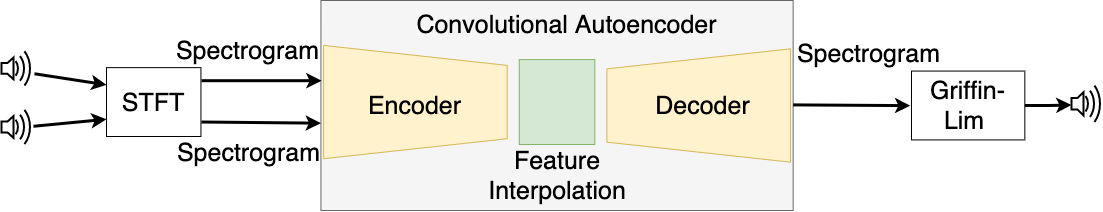
\includegraphics[width=\textwidth]{images/approach/Toolchain.png}
\end{figure}

Starting on the very left, two audios are taken and have to be brought into a suitable representation for this type of network. As audio is in its raw form a time-continuous signal and the input for convolutional networks are of a different shape (e.g. images) some pre-processing has to be done. In this case the short-term Fourier transform (STFT) is applied in order to generate a spectrogram, that shows the frequency spectra over time. The frequency spectra contain on the one hand the magnitude (power) of the frequencies but also the phase information. For this purpose, only the magnitude data is used, as recent publications stated that it contains the most descriptive data of an audio (spectrogram). The autoencoder model then takes the magnitude data as input, from which a compressed representation with the essential features gets generated by the lefthand (encoder) side. Having those features of two different audio samples, those get linearly interpolated, to generate one feature vector representing the "mixed" features of two instruments. This new vector gets passed through the righthand (decoder) side of the network, which regenerates again spectral magnitude data of the same dimension as the input. In order to obtain a "playable" audio sound, it gets transformed back into time domain with the Griffin-Lim algorithm \cite{Griffin1984} or the inverse short-term Fourier transform (ISTFT). The latter will be applied if there was no interpolation in the embedded space, as the phase information can be reused. Corresponding terminologies as well as a detailed insight into each step and its functionalities are given down below in the following points.

\section{Pre-processing}
\label{sec:app_pre-processing}
Pre-processing is the task of preparing raw data for a specific purpose. Moreover it is an important component of machine learning techniques, with respect to training neural networks. Deciding which pre-processing technique(s) to use on the one hand depends heavily on the type of ML problem that has to be solved or even the training method that is chosen, but of course also on the type of data itself. As written before, for this work a neural network consisting of convolutional layers has been chosen to be applied to the problem of neural audio synthesis. As convolutional neural networks are known for image processing tasks, they also can be applied for audio data, which has already been outlined in recent works in this field (see chapter \ref{cha:related_works}). In contrast to image data which most of the time has a 3D shape (width x length x RGB-colors), raw audio has a different structure in its data representation, as it is a time-continuous signal (1D-shape). In order to bring the audio data in a similar shape, it has to undergo some pre-processing steps. Some representations of audio that have an image-like shape and that got proven beneficial regarding neural audio synthesis, include e.g. log-magnitude spectrograms or Mel-spectrograms but also chromagrams and Constant-Q Transform as stated by \cite{choi2018tutorial}. Taking recent works into account, this work chooses to use the first representation as this one also got used more frequently and had promising results. As for comparison in the experimental part of this work, also the use of Mel-spectrograms will be assessed and discussed concerning the synthesis task and the performance of the neural network. 

As the practical part of the project to this thesis is implemented in Python, a special library was used for the pre-processing part. For this part the library \textit{librosa} \cite{brian_mcfee_2022_6097378} was used, as it provides practical functions for audio processing, that were considered useful for this work. The functionalities of calculating spectrograms (STFT) but also transforming spectral data back into time domain to generate playable audio data (ISTFT, Griffin-Lim) are of special interest here.


\subsection{Spectrograms and STFT}
Spectrograms represent a 2D-representation of an time-continuous signal, which essentially shows the presence and change of frequencies over time. Like previously said, there exist different forms of spectrograms e.g. log-magnitude and log-mel spectrograms. Especially speaking of the log-magnitude spectrogram whose calculation is based on the short-time Fourier transform (STFT) and thus on the Fourier transform. The Fourier transform takes a frame of $N$ values of an (audio) signal and transforms it from the time domain into the frequency domain. Generally said, that the bigger the frame, the better is the frequency resolution. What this means in terms of calculating the spectrogram, will get outlined shortly. What's also important to mention at this point is, that the result of the Fourier transform consists of an array of $N$ complex numbers, which are mirrored around the middle. Every complex number in this array stands for a so called frequency bin in the signal. The real part of these numbers would represent the power/magnitude of this "bin" and the imaginary part gives information about the phase. Coming back to the frequency resolution, this for example means that when taking a one-second signal with a sampling rate $SR$ and performing the Fourier transform with length $N=SR$ on it, this would yield an array of $N$ values. The first value in the result depicts the signal's offset whereas all values from 1 to N/2 are the frequency bins with a resolution of 1 Hz per bin. This means that each of these bins shows the magnitude and also phase of each frequency from 1 to N/2 Hz. The ongoing values in the result show the same values except they are mirrored, as they depict the negative frequencies. Because of this behaviour, the second part can be omitted for further use. Now these values just show the frequency spectra of one time frame and do not incorporate more information about the change. To overcome this shortcoming the Fourier transform can be applied to a series of frames of the signal in order to obtain multiple frequency spectra over time that are depicted as a spectrogram.

The calculation of multiple frequency spectra over time is done via the so called short-time Fourier transform. This form of calculation is widely used for pre-processing of audio data for ML-tasks (see chapter \ref{cha:related_works}). When applying this transform, a few parameters have to be considered, as those influence the result but also the quality for the later workflow. As \textit{librosa} is used for the sound processing steps, the mentioned parameters are specifically concerning this library. One of the the most important parameters is \texttt{n\_fft} as it specifies the actual length of the signal frame, on which the FFT (fast Fourier transform) gets applied. This parameter therefore influences the frequency- but also time-resolution in the final spectrogram. Regarding the official Librosa documentation, this should be a value of a power of two, as it speeds up the computation of the FFT. Another important parameter would be the \texttt{hop\_length}, which defines how many audio values are between the beginning of the first and the following frame. This means that when defining this parameter to \texttt{n\_fft/2} this would yield a 50\% overlap of the following frame. Modifying this parameter would mean to either increase or decrease the overlap and also the amount of time columns in the result, as more overlapping frames occur. The overlap of the frames is also coherent with the chosen window function for the STFT. As every time when the FFT gets applied to a frame, this one gets multiplied with a so called "window". Multiplying a signal frame with a window has to be done, as the FFT assumes, that the transformed signal is periodic (repeating itself infinitely) \cite{heinzel2002spectrum}. This becomes problematic when the input signal does contain frequencies that may not directly fall into a frequency bin, due to the FFT's frequency resolution. Due to the assumed cyclic continuation the Fourier transform will 'think' that there is a discontinuity and will spread therefore the power over the spectrum. There are various window functions such as "Hann", "Hamming", "Blackman", etc. which start at (almost) zero, rise to a maximum in the middle but fall again to (almost) zero at the end (symmetric). Multiplying the signal frame with such a window function helps to overcome this issue as it removes the discontinuity. Which window to chose depends on the use-case of the application, whereas throughout this work a "Hann" window was chosen. It got chosen, because it is good suitable for most sound processing tasks. Moreover it reaches zero at both ends and thus eliminates the discontinuity problem. Coming back to the relation with the window overlap, if no overlap would be used a lot of information of the signal would get lost. This is because when multiplying the signal frames with the window functions, this would result in very small or zero values at the beginning and end of the frame \cite{heinzel2002spectrum}. When having overlapping frames this issue would be corrected. Important here is again the amount of overlap as this is dependent on the window and its wideness. Using the "Hann" window a common value for the overlap would be 50\% which was also considered throughout this work. This value is also beneficial later on when performing the inverse transformation, back into time domain, but more on that in section \ref{sec:app_post_processing}. Beside of these parameters some more exist, for example for specifying the padding of the signal whereas in this work a constant padding on both sides of the signal has been used, which is also the default setting.

Now having knowledge about the STFT and its parameters, it can be applied to a signal to generate a spectrogram. For example by using an audio sample with a sample rate of 16 kHz and applying the STFT with a \texttt{n\_fft} value of 1024 and a \texttt{hop-length} of 512 this would result in a spectrogram with a frequency resolution of 15,625 Hz and time resolution of 64 ms. As explained before, the values of the result consist of complex numbers which contain the magnitude but also the phase at each frequency bin. By setting this result absolute, or calling the function \texttt{librosa.magphase(spectrogramm)} the real magnitude data can be obtained, whereas the latter also retrieves phase information in a separate vector. The magnitude here displays the energy values of the spectrogram, whereas for further processing and also to be better displayable those get converted into a dB-scale \footnote{normally the magnitude would need to get squared to obtain the power, but in this case magnitude without squaring was taken}. This function also takes a reference value that is set to 0 dB, which in this case will be the maximum value of the magnitude spectrum. As for post-processing when converting the dB-scaled data back into energy, also a reference value is needed, this one gets preserved, in order to get the same scaling as in the original input. Finally when having the log-mag spectrograms in dB, those were considered for the training of the neural network afterwards. An example of a log-mag spectrogram can be seen in figure \ref{fig:spectrogram}. This spectrogram shows the frequency spectra of a guitar sample over time. It can be seen, that at the beginning and at the end there are broadband spectra, which represent the guitar stroke (transient) at the beginning and the noise of damping the strings at the end. As also the phase information was obtained when calculating the magnitude data, this one was also preserved next to the energy reference value for the recreation of signals, as it is needed there (this will mainly affect the recreation of single samples, without interpolation in embedded space, but more on that later on).


 \begin{figure}[htb!]
	\caption{STFT log-mag spectrogram of a guitar note.}
	\label{fig:spectrogram}
	\centering
	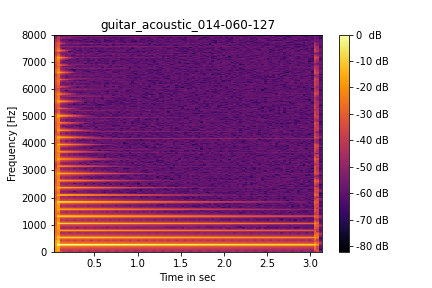
\includegraphics[width=0.8\textwidth]{images/approach/guitar_acoustic_014-060-127.png}
\end{figure}

This section describes the general workflow of the pre-processing from taking a signal and converting it into a spectral representation. This workflow is a basis on which different experiments with different parameterization (size of n\_fft, etc. ) of the calculation of the spectrograms but also with additional steps (log-mel scale, additional framing, etc.) are being made. Those steps will get mentioned later on in chapter \ref{cha:Experiment} when describing the experimental part of the thesis.

\section{ML-Model}
\label{sec:app_model}
The main or core component of every machine learning project is of course the model itself, as it achieves the main task of prediction or inference to a given problem. Those models exist as different technologies that perform regression tasks or even classification tasks. Dependent on the use case, but also the kind of data that is present, different models are better suited or not. To enumerate technologies, there exist the KNN algorithm, Decision-Trees, Random Forests, Support-Vector-Machines (SVM) but also neural networks which can be applied in a variety of use cases. Especially the latter, the neural networks, are able to achieve a variety of different tasks, as they are highly adaptive regarding their topology, used layers, but also their size and shape. This variety of different tasks spreads across different domains, including images and audio. 

\subsection{Neural Networks - Introduction}
Generally said a neural network can be seen as a graph of connected nodes  with numeric values that can achieve transformations between patterns using message-passing algorithms \cite{Jordan1996neuralnets}. Those nodes are commonly structured in layers, where there especially exist certain nodes or even layers that are seen as input nodes/layers and some as output nodes/layers. Between the input and the output there can also exist so called hidden layers, expanding the depth of the network. The links between the nodes, that are also called neurons, are connected via links, that are parameterized with weights, that get optimized using learning algorithms. Each neuron receives its weighted input (activities) of its connected predecessors, which get converted into a single output that gets broadcast to all its connected successors \cite{hinton1992neural}. The latter involves a so called input-output function which is also commonly known as activation function (e.g. ReLU, Sigmoid, Softmax, etc.). Important to know is that the weights on the connections define how much this value influences the input of the connected node. 
When a neural network is trained to a specific problem (e.g. classifying certain images), using predetermined training data, the output of the neural network is compared with the desired one, resulting in a certain error (metric). To minimize this error, the weights in the network are adapted by backpropagating the error through all the layers, to the beginning. On this way it changes the influence of certain connections and therefore the overall outcome. This procedure is repeated on all training data over several iterations, until the error becomes low to produce the desired output. The initialization of the network and its weights is often random, which also means that every training run starts and progressses differently.

Depending on the problem at hand, neural networks can be trained using labeled data (supervised) but also just by minimizing a cost function (unsupervised) \cite{oshea2015introductionConv}. More details on the learning will get mentioned later on when explaining the model itself. 

\subsection{Convolutional Neural Networks}
\label{subsec:app_conv}
In this approach, due to the promising usage in existing solutions, a convolutional neural network has been chosen as the model. Convolutional neural networks are a type of network, that get primarily used for tasks in the image domain for example to recognize patterns in pictures or classification, but also like seen in chapter \ref{cha:related_works} for image style transfer. They have the advantage over traditional neural networks, that they can deal with the dimensionality of pictures (width by height by colors/depth). The layers containing convolutional nodes have kernels as learnable parameters \cite{oshea2015introductionConv}. Those kernels, if taking a 2D-convolutional layer, are normally small in width and height (e.g. 3x3) but span the whole depth (channels) of the input (in the case of RGB pictures depth of three). Those kernels calculate the scalar product for each value contained in the kernel and the input map. This yields, having e.g. a 3x3 kernel operating on a 3x3 field, in a single value. This value is the weighted sum of the kernel's values and from those of the input vector. This operation will be applied to each 3x3 field along the spatial dimension of the input, resulting in a smaller activation map. One can also apply padding around the input to preserve the dimensionality. Furthermore a stride can be defined, which defines how much these convolved fields overlap, as using a bigger stride would result in a smaller overlap. Having also a smaller overlap would result in a much smaller activation map. 
For example taking a 7x7 input, by applying a 3x3 kernel with no strides and also no padding, this would yield an output field of 5x5. With a padding of 1x1 the output would be of the same size. Finally if the stride would be 2, the output field would be of 3x3.
Through training of the network and back propagating the error, those values in the kernel get adapted in order to learn certain important features or patterns on which a classification or pattern recognition can be made (easier). As it got described for 2D convolutions, depending on the input dimensionality it can also be applied as 1D convolutions or even 3D convolution. 


With the knowledge that such convolutions are successful on image data, those can be also applied on audio provided in the shape of a spectrogram. As described in the previous section (see \ref{sec:app_pre-processing}) spectrograms can be described in a "picture-like" shape having the dimensions of frequency by time with a depth of one. Speaking of that, the spectrogram can be seen as a grey-scale image. The energy in different frequency bands over time with its variations, can be seen as "recognizable" patterns. 
Taking a 2D convolution, the kernel (e.g. 3x3) takes a 3x3 frame of frequency by time which results in one value. Summed up, this results in an activation map smaller or equal (if zero padding is used) than the input. After training on different samples and iterating several times, this activation map would contain the most significant features or characteristics of the spectrogram for example when training on classification.
Depending on the chosen hyperparameter for the amount of output channels (depth), the resulting activation map can be of depth one or even deeper. 

As mentioned before, each neuron in a neural network has an activation function, which is also the case for convolutional neural networks. As there exist different kinds of activation functions, for this approach mostly ReLU (Rectified Linenar Unit) activation functions got used but also LeakyReLU. Additional to this activation function, BatchNormalization gets applied after each convolutional and ReLU non-linearity component. The choice is mainly based on already existing approaches like from \textit{Ramani et al.}\cite{Ramani2018} and \textit{Engel et al.}\cite{Engel2017}, as it was proven to yield promising results in combination. According to \textit{Ioffe and Szegedy} \cite{ioffe2015batch} applying Batch Normalization also improves the training speed (number of iterations/epochs) and enables the use of much higher learning rates. Furthermore it acts as a regularizer, so that overfitting-reducing technologies, such as Dropout, can be omitted.

\subsection{Autoencoder}
Neural networks exist in different shapes and compositions, depending on the desired work it should fulfill. Whereas some networks e.g. for classification of a given input, might reduce the width of the layers towards the end, some are designed to have a so called bottleneck. This means that this kind of network contains a smaller central layer then the input, but at the end again a bigger layer (eventually same size of input layer) \cite{hinton2006autoencoder}. Those networks are called autoencoders, in which the first part of the network (until the smaller central layer) gets called "encoder". The second part beginning at the small central layer, that is getting bigger towards the end, gets called "decoder". These parts are called this way, as for the encoder part, it "encodes" the high-dimensional input data to a low-dimensional representation (output of small central layer). The counterpart is therefore called "decoder" as it decodes the low-dimensional data, to bring it again to a higher-dimensional representation (mostly same as input). The lower dimensional output of the small central layer, can be named differently, as for example "code", what \textit{Hinton et al.} does when describing the concept of autoencoders in his publication \cite{hinton2006autoencoder}. Some other common names would be e.g. latent space, embedding space, encoding or embedded data. This principle of dimensionality reduction therefore means, that the encoder part extracts the most important or characteristic data, from which the decoder is able to reconstruct the input data.

In the related works chapter \ref{cha:related_works} a few works have made use of this principle to extract "characteristic" features for audio data and synthesize audio from it, by altering them. This knowledge encouraged this work to also make use of this principle to synthesize audio by using autoencoders. Especially when having the extracted audio features as encodings, those can be modified (easier), to in order synthesize novel sounds from them using the decoder part of the network. 
Combined with the knowledge to apply convolutional networks to audio spectrograms and the advantages of autoencoders to extract features from the input, the model in this work is designed as a convolutional autoencoder. Also the works of \textit{Ramani et al.} or \textit{Engel et al.} made use of these kind of network to generate novel sounds. Figure \ref{fig:app_autoencoder} shows the basic autoencoder network structure which is used throughout this thesis. To be mentioned, the whole implementation of the neural network for this work has been achieved with the deep learning library PyTorch \cite{paszke2019pytorch}.

\begin{figure}[htb!]
	\caption{Basic autoencoder structure used throughout this thesis.}
	\label{fig:app_autoencoder}
	\centering
	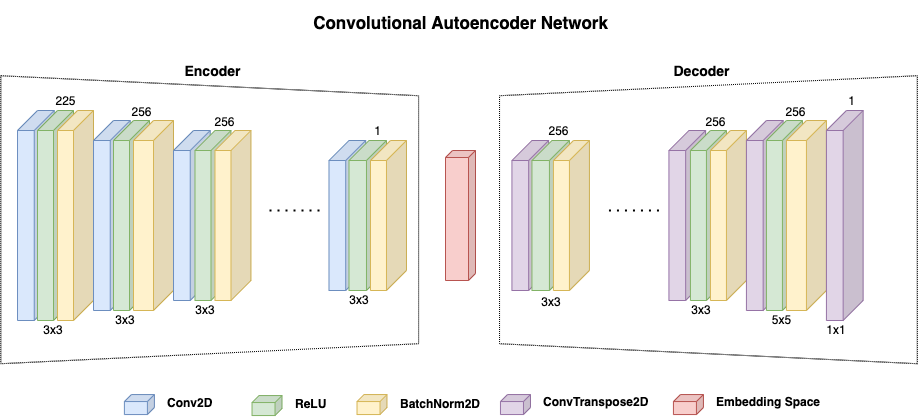
\includegraphics[width=\textwidth]{images/approach/autoencoder.png}
\end{figure}

In figure \ref{fig:app_autoencoder}, the depicted autoencoder, gives an insight of which components and layers it is composed of. The amount of layers as well as the parameters shown in this sketch, are just an example, as throughout the experimental part, those get varied. Therefore, the dotted lines in this figure act as a placeholder for possibly more layers on each side of the network. The numbers above the individual layers represent the amount of output channels (depth) and those on the bottom represent the kernel size. It has been mentioned that in this approach the convolutional layer gets equipped with ReLU activation functions and batch normalization. This also gets visualized in this figure, where each layer is shown as a combination of sub-layers that incorporate those three components. Speaking of the composition of the layers, it can be seen in the decoder part, that instead of a convolutional layer, a convolutional transpose layer is used. That is because of the nature of convolutions, as their output is always smaller or equally sized, which has been mentioned under point \ref{subsec:app_conv}. As the decoder part generates output that is bigger than its input, the layers have to perform upsampling. In convolutional nets this is typically done via the convolutional transpose layer.

This transposed convolution is not the reverse operation of a convolution, but it is more of a operation to recover the shape from the convolutions input. \cite{dumoulin2018guideconv} Taking the convolution example from above, by taking as input a 5x5 field and applying the transposed convolution with a kernel of 3x3, this would result in a field of 7x7. The equivalent of this operation would be a convolution with the same kernel, on an input of 5x5, with 2x2 padding (padded input = 9x9), as this would result in a 7x7 output too.
When in the convolution, striding was applied, this also works for the transposed convolution. Again when having the 3x3 input, by applying a 3x3 kernel with a stride of 2, this again results in a 7x7 output field. To be mentioned, the striding parameter for the transposed convolutions defines how much zeros are added between the values of the input. This means, when taking the previous example, that the 3x3 input gets one column respective one row of zeros inserted after each value to result in a 5x5 field.

With this knowledge, convolutional transpose layers are best suited to be in the decoder part of convolutional autoencoder networks. Coming back to the architecture of the convolutional autoencoder in figure \ref{fig:app_autoencoder}, those convolutional transpose sublayers are also coupled with ReLU activations and batch normalization, with an exception to the last layer.

Having this kind of autoencoder for this approach and the idea to extract features of spectrograms using convolutions, this models task is to encode and decode spectral audio data. The network is therefore configured to produce an output of the same dimensionality as the input of the encoder. Like mentioned above, the output should be a reconstruction of the input, that gets inferred by decoding the extracted features in the embedded space. To achieve this goal of reconstructing the input, the network has to be trained through minimizing a specific error. In some cases also maximization is desired, but is dependent on the error score and the desired outcome. In the case of an autoencoder, this works by comparing the output of the decoder with the input of the encoder, by calculating the difference. Generally said, depending on the outcome and the goal of a training, there exist different metrics like mean squared error (MSE), root mean squared error (RMSE), mean absolute error (MAE) but also more specific formulas. Throughout the literature, those error functions are also often called cost (functions) or loss (functions). For the experimental part of this work, the choice has been made to use MSE as the error metric, as it has been used successfully by some existing works. 

To minimize this error an optimization of the network has to be made, which will be done through backpropagating the error score. Through this step, the parameters (weights, bias, convolutional kernels, etc.) get adapted according to the error, which in the best case improves the score and thus the output of the network. In this work the output of the network are reconstructions of spectral data. As having the encoder-decoder structure, this output data is reconstructed through the decoder, which takes the encoder output as input. As mentioned before, this generated data of the encoder is a compressed vector, consisting of the most significant information extracted from the input. Depending on the configuration of the network, especially the encoder part, this vector can be of different sizes. This is because when using more convolutional layers with strides, the output of each layer gets more downsampled, which results in a smaller encoding. As a consequence, the decoder part has to learn to regenerate spectral data from this encoded vector. This vector therefore is a compressed representation of the models input, which contains the most significant characteristics of this specific spectrogram and further on, of the sound. All in all regarding the learning, it can be said, that the encoder learns to extract essential features, from which the decoder learns to regenerate the input as well as possible.

Altering those encodings has therefore the consequence, that the output of the decoder is different, and thus will be a novel, synthesized sound. More on how it should get altered is discussed later on.
Choosing the right compression is also an important part that influences the outcome and thus the quality of the desired model output. Too much compression may lead to the fact that the decoder has too little information to infer the desired spectral output, which in order results in poorer quality of the resulting audio. On the other hand having less compression results in embeddings being not significantly smaller then the input, containing less important data too (e.g. noise). It also may become more difficult to alter those encoded vectors. Throughout this work, different amounts of compression have been applied in the experimental part, which get discussed later, including the impacts and observations made on that. Knowing those properties and behaviour of the autoencoder model strengthens the idea of applying autoencoders for the use of neural audio synthesis.


\subsection{Optimizer}
Coming back to the training process, where the network gets optimized, in order to minimize a certain error function. For this optimization, different strategies exist, where hyperparameters such as learning-rate or weight-decay play an essential role. Those optimizations are on a large scale, stochastic gradient-based techniques, to which algorithms such as stochastic gradient descent (SGD) or Adam can be counted. Those algorithms influence and improve the convergence which means to find a minimal error. Throughout this implementation the Adam optimizer \cite{Kingma2014} has been chosen, as it is used widely in recent publications where promising results could be achieved. Also regarding the training process in this work, Adam optimizer has proven to be advantageous, in contrast to SGD. The parameters that have been found to have the most impact on the optimization process during training, are the previous mentioned learning-rate and weight-decay. To be mentioned, the learning-rate specifies how "fast" the model actually learns while weight-decay works as a penalty for the weights optimization to prevent overfitting. If the learning rate is chosen rather large, then the network learns faster, but because of its big steps or jumps, it could miss the optimal solution in the solution space. Also it could happen that when a local optimum is found, that it "jumps" out again. In this case a smaller learning rate would be desirable, as it makes smaller steps. Choosing it too low would end up in a slow training where also large areas of the solution space are not visited. The latter leads to a training process stuck in a local minimum. Therefore it is important to choose the right size of learning rate, but this issue depends also on the problem size and type of network. In this work different learning rates have been applied throughout the experimental part where also different findings could be made, but this will be shown and discussed later on in this thesis.\\
With this knowledge, it can be stated, that a high learning rate could be advantageous at the beginning of the training process, in order to rather find a global optimum and explore the solution space. In order to prevent jumping out of a minimum, a smaller learning rate would be desirable later on in the training. For this case, there exist some mechanisms to decrease the learning rate later on in the training, especially when detecting oscillations of the error due to a too large learning rate.\\
In this works' implementation, for the start of the training a specific starting learning rate has been set, while throughout the training it gets adapted, when no more optimization and eventual oscillation gets detected. 


\section{Synthesis of novel sounds}
\label{sec:app_interpolation}
Having now covered the important properties of the pre-processing but also of the applied machine learning model, this section explains the methodology to synthesize novel sounds. In the chapter \ref{cha:related_works} where related works got discussed, an insight could be gained, on how different works tried to synthesize audio with their neural networks. For example \textit{Colonel et al.}\cite{colonel2017improving, colonel2018autoencoding, Colonel2020} suggested in their works, to synthesize novel sounds through directly activating the innermost layer. This means after training, for the sound creation process, the encoder part gets omitted. For example in the case where they had a network with 8 neurons at the encoders bottleneck, 8 different values could get defined, within a certain range. The decoder part then created, based on its training on recreating spectrograms, spectral data that got converted back to time domain to form a synthesized playable sound. 

\subsection{Interpolation in latent space}
Having this as one possibility, to use in particular autoencoders as a tool for audio synthesis, there also exist some more interesting approaches. One of those got applied by \textit{Engel et al.} \cite{Engel2017} but also \textit{Roche et al.} \cite{roche2019autoencoders} where they also made use of the latent space encodings. Contrary to omitting the encoder part, those works aimed to utilize the whole network, as no direct activation of the innermost layer is considered. Instead the authors proposed to take the encoded values of two different audio samples (possibly two distinct instrument) and combine them via linear interpolation. The interpolation process yields a vector of interpolated values. This new vector can be seen as a modified encoding, which gets processed by the decoder part, resulting in spectrogram-like vector. The result of this process is then a synthesized spectrogram, that aims to contain features of the two input sounds.

As the latter methodology corresponds the most with the initial idea, to synthesize audio based on the characteristics of two instruments (e.g. guitar and synthesizer), this method was chosen to be implemented to carry out experiments on the creation of novel sounds.

To explain this method in more detail, the encoded vectors of two audio samples serve as the basis. Then each of this vector is taken, to interpolate a value that lies on a linear line between the value at a given index in one vector with the corresponding value of the same index in the second vector. To mention at this point, those vectors are of the same length. The result then is a new array containing the interpolated values of those two vectors. This procedure gets repeated for each encoded output of one sample with the corresponding output of the second sample. Knowing the fact that those encoded values represent the most significant features and probably the characteristics of the note, the result can be seen as a combination of those characteristics. Decoding those will then end up in having a spectrogram containing the characteristics of both instruments. How this procedure and its results look like, with the actual experiments, is shown later on in this work. 

\section{Post Processing}
\label{sec:app_post_processing}
It has been discussed, that regarding neural audio synthesis, the audio data can appear in different shapes. As there exist approaches, that focus on time domain signal like the WaveNet-style autoencoder from \textit{Engel et al.}, there also exist those who operate on spectrograms using convolutional networks. As mentioned before, this work emphasizes the use of a convolutional autoencoder, that takes spectrograms or spectral data as input. In the case of this autoencoder, the output is of the same shape as the input and therefore also a spectrogram. To generate again a playable or listenable audio, this one has to get converted back into time domain. There exist many different methods, to achieve this, while this also depends heavily on the data that is present. As stated in section \ref{sec:app_pre-processing}, when spectrograms are calculated via the STFT, the output vectors are complex valued. To be mentioned, that without modification or further utilization, via the inverse STFT (ISTFT), this result vector can get converted back into time domain without loss. For achieving this task, it is necessary that the magnitude but also the phase information has to be present, combined in a complex number. As this autoencoder just operates on the magnitude data of spectrograms, there is no phase information present in the output of the network. At this point, multiple ideas can be applied, depending of what is done throughout the process. This means that when there is no modification in latent space, i.e. value interpolation, the original phase information can be reused while applying the ISTFT. As mentioned previously the phase information gets preserved for exactly this case. 

In the second case, where modification steps are performed, like here the interpolation of two sounds' embeddings, there is no phase information present that can be used. To overcome this issue, there exist techniques that can approximate the phase information. One of those techniques, which is also probably one of the most prominent ones, is the Griffin-Lim \cite{Griffin1984} algorithm that tries to estimate the time domain signal based on just the magnitude data. With this algorithm the phase gets randomly initialized, and with alternating forward- and inverse STFT, estimated. For the calculations of the audio signal, again the python library \textit{librosa} \cite{brian_mcfee_2022_6097378} has been used, as it provides the inverse STFT but also implements the Griffin-Lim algorithm. According to the documentation of \textit{librosa}, a so called "fast" Griffin-Lim algorithm is applied, which got developed by \textit{Perraudin et al.} \cite{Perraudin2013}. The difference here is, that this one utilizes a additional momentum parameter which helps to accelerate the convergence of the estimation. 

Some further note here, as when the pre-processing steps (see section \ref{sec:app_pre-processing}) have been examined, that some certain parameters have to be taken care of. These are especially the \texttt{n\_fft}, \texttt{hop\_length} but also the \texttt{window}. It has been mentioned, that e.g. the \texttt{hop\_length} was chosen to be half of the \texttt{n\_fft}, to ensure a 50\% overlap of the STFT frames. Furthermore the "Hann"-window was chosen, to be multiplied with the signal frames, to avoid discontinuities. Again, those also appear in the inverse STFT as well as Griffin-Lim. In order to obtain the best result, it is important to apply the same values with those parameters. As the inverse Fourer transform gets applied to each vector in the spectrogram, this results in single time domain frames that have the length of \texttt{n\_fft} (original length). With the knowledge of the window and the overlap, those single frames, get "overlap-added", which results again in the full length audio sample. 

Before applying the the inverse calculations on the autoencoders output, it has to be considered that the autoencoder works on the db-scaled magnitude. As a consequence the output therefore is also db-scaled. To apply the inverse calculations, the output becomes energy again. For this case a reference value has been preserved from the pre-processing stage, in order to obtain the (almost) same scaling again in the output signal. For the experimental part some more steps also got applied, like scaling the energy according to the average energy present in the original spectrograms. This step should also correct and improve the resulting sounds. More on that in chapter \ref{cha:Experiment}, but also later on when examining and discussing the results.


\section{Dataset}
\label{sec:app_dataset}
As machine learning models including neural networks, have to get trained, in order to deliver accurate results, data is needed on which it should get trained on. To get compelling results, it is not only important to have an appropriate model configuration or pre-processing chain. The choice of an appropriate dataset therefore is also of high significance. As seen in related works, datasets can either be self-generated or taken from a publicly available data source. As in the case of this work, the model operates on audio data, a dataset of musical notes is desirable. Generating sufficient data, by oneself, is a task that would take a significant amount of time. Not only as this dataset preferably should contain a large amount of audio samples, those also should be highly diverse such as different instrument sources or different pitches. Not only is it an advantage for the training of the neural network to have lot of samples and diversity, as it helps to improve the learning process and generalization within the neural networks. Moreover it is also advantageous for this kind of work, as when having many different instrument sources and available notes, more interesting combinations with regard to audio synthesis can be made.

\subsection{NSynth Dataset}
Exactly for this kind of approach a large dataset consisting of instrument samples called "NSynth", has been made publicly available by \textit{Engel etx al.} \cite{Engel2017}. This dataset consists of a total of 306.043 musical notes that have a unique pitch, timbre but also envelope and has been created for the idea of neural audio synthesis. This amount of musical notes incorporate monophonic audio snippets, sampled at a rate of 16 kHz, of 1.006 different instruments. Every note is of a specific pitch, ranging over every note of a standard midi piano (21-108). This results in having 88 different pitched notes, in the best case, as not every instrument is capable of producing all different pitches. The average amount of pitches is therefore, according to the scientific publication, 65.4 per instrument. With more detail, each audio sample belongs to a certain instrument family which could for example be a keyboard, guitar, organ, bass, brass and so on. Further on they can be distinguished by their source, being either produced acoustically, electronically or synthetically. All these specifications make this dataset highly attractive for this kind of work, besides being publicly available\footnote{\url{https://magenta.tensorflow.org/datasets/nsynth}} for free and already successfully used for neural audio synthesis. Regarding the use for machine learning tasks, on their website, they provide the dataset already split up into a training, validation and test set which do not overlap at all. To specify, the training set consists of 289.205, the validation set of 12.678 and the test set of 4.096 examples. For this purpose, it has been chosen, to take these splits as they are, for the training, validation and finally testing stage.
\chapter{Experiment}
\label{cha:Experiment}
This section describes the experiments conducted in order to be able, to answer the defined research questions. In the previous chapter (\ref{cha:Approach}) the general methodology used technologies got described, to gain an understanding of the implementation and its components. Based on this knowledge and implementation, some experiments got conducted, that provide interesting results and meaningful insights into this approach of neural audio synthesis. For the purpose of this thesis, some research questions have been defined, for which the following experiments, deliver the answers, which get discussed later on when showing the results.\\

\noindent Those research question are defined as the following:

\begin{itemize}
    \item \textbf{Is it possible to create novel sounds based on the characteristics of two instruments, by using ML technologies such as convolutional neural networks?}

    \item How do the pre processing steps influence the quality of the training, but also the quality of the output?

    \item How does the configuration/composition of a neural network influence the quality of the output?

    \item What are the information that are learnt from the neural network?

    \item By using audio spectrograms, are they suited best to achieve this task?
\end{itemize}

In the last section, when describing the different technologies, it has been mentioned, that they can be parameterized in order to influence the outcome of this work. Furthermore some additional steps can be introduced that have a significant impact on the result. This section therefore describes, how the proposed methods were utilized, in order to answer the above mentioned questions. Furthermore those experiments, should deliver some interesting insights, on how different configurations influence the workflow but also the final result being a synthesized audio. Those experiments span almost every stage from the pre-processing until post-processing. 

\section{Implementation Environment}
In the previous chapter it has already been mentioned, that this approach is developed in python using specific libraries. To shortly mention, for pre- and post-processing the python audio-library \textit{librosa}\cite{brian_mcfee_2022_6097378} has been chosen, as it provides all necessary functionalities that are needed for the approach and experiment. For all steps regarding the neural network model such as configuration, training, inference etc., \textit{PyTorch}\cite{paszke2019pytorch} has been utilized. The project though has been implemented and applied on two different machines, depending on the task that has to be done. Generally speaking, the toolchain compromised of all stages, has been developed on a local machine running python, except the training itself. 

Speaking of that, the training has been mainly performed on a remote "jupyter-notebook" that has access to high-performance GPU resources. Not at least, as in the case of training a convolutional neural network, this is a rather time and computational power-consuming task. Of course, this not only depends on the kind and complexity of the network, but also on the amount of data that is used for the training. Furthermore using GPU-acceleration means to significantly have more computation power and speed, as its applying parallelism. Using the local machine, just the CPU could be utilized for training, which would mean that training is done sequentially and thus significantly slower while the local machine has to be awake constantly. For the training on the remote instance, the pre-processing also gets done there as the data is directly loaded there. 
As just the training is performed remotely, all other steps, including the evaluation towards audio (re)synthesis having the trained model, gets again done locally. Not at least, as no time-consuming tasks have to be made, but also as its more convenient, as the remote service is not always accessible.


\section{Training}
The training, as mentioned previously, gets performed on a remote "jupyter notebook"-service with access to a GPU. As outlined in the previous chapter, for the whole experiments, the NSynth data set proposed by \textit{Engel et al.}\cite{Engel2017}, gets used. As is well known this dataset is already split into a training, validation and test part. For the training on the remote notebook, the training and validation data set will therefore be used, which in order also get pre-processed there. As a side note, in the beginning of the project, the training was just held locally, with a small subset of the already small test set (mostly of one instrument). This was just done to make a low-level proof that the autoencoder model can produce meaningful results. 

\subsection{Training configuration}
To take a closer look onto the training process, this one consists of several important stages and components. First of all the PyTorch-model, defined as a class, gets initialized. As an metric is needed, to measure the error of the output, the mean squared error (MSE) gets utilized. This error metric calculates the difference between all values of the desired and actual output, squares them, and takes the average over all. Furthermore to optimize the network, as explained before, the Adam optimizer gets applied, in which the (starting) learning rate, but also the weight decay gets defined. The right learning rate depends here heavily on the amount of training data but also complexity of model. In the case of this work, this means it is in the range between $1e-5$ to $1e-7$. In chapter \ref{cha:Approach} it got also mentioned, that a technique to minimize the the learning rate, during the training process gets utilized. This function called \texttt{torch.optim.lr\_scheduler.ReduceLROnPlateau(...)} reduces the learning rate, by a given factor, if within a certain patience period (epochs) no optimization gets detected. This method, improves the training process as further convergence can be achieved. Of course for the training process, the pre-processed training and validation data set has to be loaded. To mentioned, the pre-processed data gets calculated and stored on disk, in advance, to not always have to run through it. for the training it therefore gets loaded and brought into the desired shape for the corresponding model. This shape gets varied throughout the experiments, to observe its impact on the training process but also quality of the output. As this also depends on the chosen network, this gets described later on in this chapter. For the sake of training, this gets done with the training dataset, as well as for the validation dataset, as after each epoch the model gets evaluated on a held out validation set, to check the error on never seen data.
The data in the right shape, has to be converted to a tensor and in further notice, to a (custom) dataset object. Finally a so called "DataLoader" has to be initialized, either for the training but also for the validation. In this DataLoader the batch size can be specified, whitch is an important parameter regarding the training. Throughout a few batch sizes, have been tried out, whereas in the end, the prefered batch size was 32. This means that the input data, gets portioned in equally sized chunks of 32 tensors, that get fed into the network at once. Further on it can be set, that after each training epoch, the dataset gets shuffled. Setting this to true, the samples in the batches are in a different order and constellation. Otherwise, the batches consist always of the same data in the same order. Throughout the experiments, this setting was proven to be advantageous regarding the convergence of the model, as the error could be more minimized (see chapter \ref{cha:Results}).

\subsection{Training Execution}
Having the configured dataloaders, which are also iterables, it is possible to iterate over the batches of the dataset. Before the training begins, a number of epochs has to be set, which defines how often the training should be performed on the whole dataset. In advance it cannot be said, how many epochs are needed, therefore a preferably big number gets chosen e.g. 1000. To clarify, the training never runs until the final epochs, as it get stopped at a point, where the result is sufficient (more on that shortly). In each iteration, the corresponding batch of data will get input into the network with a forward pass which calculates an output. This output gets compared to the desired value, which is in this case the same as the input, and further on the error gets calculated. Further on the gradients get computed and optimization via parameter update is done. The loss value gets added up, and after all batches are done, the average loss gets computed, to show the progress. 

After all train batches have ran through and optimization is done, the model gets validated using the held out validation set. This one is also equally batched, and runs through the same process, except there is no optimization. Here there error is just calculated to see, how the model performs on data that is not used for training and therfore never seen before by the network. This technique helps to prevent to overfit the training data, which would be signalized through an increasing validation error despite training error gets smaller. Having the validation error after each epoch, this value gets used for the learning rate scheduler to decrease the learning rate if the error does not decrease in a certain period. 

 To ensure to have a sufficient trained network, the error scores get observed periodically. If the validation score does not improve more, i.e. the network convergence stagnates, and is sufficient, the training gets stopped. Important to know that after each training iteration, which is also called epoch, the state of the model gets saved, for further use. As also the scores for each model state is known, it is therefore possible to determine the best model, having the lowest MSE-score on the validation data. This one then gets further tested and analyzed towards the applicability for audio (re)synthesis. Those further steps, which do not involve training, as well as the pre-processing regarding the evaluation data, get performed locally. 

 
\section{Initial Experiments}
\label{sec:exp_init_experiment}
In the beginning of this project, initial experiments, were done in order to make a very basic proof of concept implementation. Like mentioned before, those implementations, where entirely held on the local machine, not at least as there was no access to GPU-accelerated training. This was also possible, due to just taking a small subset of the test dataset. Of this test dataset, samples of one instrument (\textit{keyboard\_synthetic}) were taken out, and considered for test-wise training.

\subsection{Whole Spectrograms as Input}

\subsubsection{Pre-processing}
For the first experiments, all the samples of the subset, have been converted to log-magnitude spectrograms as a whole. As already known, those samples have all the same length of 4 seconds. Some samples are padded with zeros, as those do not contain audio data over the full length. As parameters for the STFT \texttt{n\_fft} of 512 and \texttt{hop\_length} of 256 got chosen. This configuration results in spectrograms having 257 frequency bins with a resolution of 31,25 Hz. Regarding the time-resolution it can be said, that each frequency vector represents 16 milliseconds of the original signal with a 50\% overlap. This procedure resulted in spectrograms with a dimension of 257x250. 

\subsubsection{Model and training}
As the spectrograms can be seen as grey-scale images, and thus 2D-Convolutions got applied, a third dimension got added resulting in 257x250x1 spectrograms.  Finally to form a dataset ready for training, all the spectrograms of the mentioned subset got concatenated to a 4D-array, which was converted into a tensor and subsequently into a dataset. The following training, was performed on 80\% of this subset, whereas the other 20\% were used for evaluation. Regarding the duration of the training, this was held for a short time (~20 epochs).

To also mention the model configuration, this consists of 4 convolutional layers in the encoder including ReLU activation and batch normalization. The decoder part has therefore also 4 layers, which contain respective convolutional-transpose layers with also ReLU and batch normalization except the very last layer. Another important detail is, because of the shape of the input, that the number of input channels has to be 1. Throughout the network, this parameter gets varied, whereas in the first layer an expansion is being made to 225, subsequently in the second to 256 output channels. To the innermost layer it gets again reduced to 100. In the decoder part, again an expansion is being made, whereas at the end it gets reduced to 1 channel again, in order to match the input size. The next graphic (fig \ref{fig:cae_2D_init}) shows the autoencoder that is used for the initial experiments. To be mentioned the kernel-size, strides (s) and padding (p) here is already the configuration for the succeeding experiment. The channels, the general structure as well as amount layers is the same for the next experiment.

 \begin{figure}[htb!]
	\caption{Initial 2D-convolutional autoencoder}
	\label{fig:cae_2D_init}
	\centering
	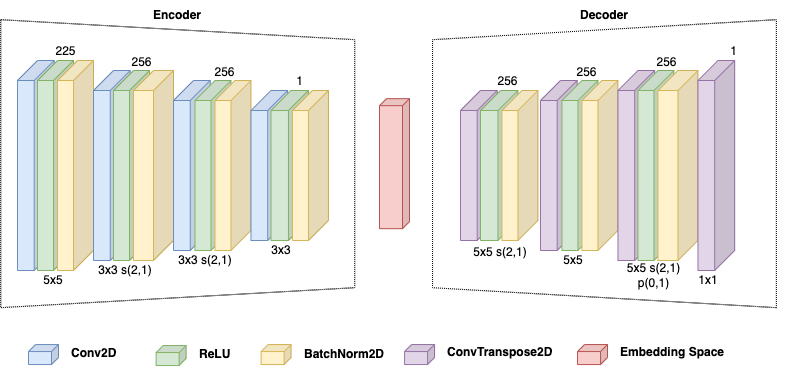
\includegraphics[width=\textwidth]{images/experiments/autoencoder_init.png}
\end{figure}

\subsubsection{Testing/Evaluation}
Regarding the evaluation of this first model, it has been tested out on the remaining 20\% of the small subset. These first experiments, consisted just of evaluating the outcome of the decoder, by passing single spectrograms through the network. By this, the ability of the network to recreate audio spectrograms got proven, which further on serves as a base for the next experiments. Regarding the final outcoming sounds, the original preserved phase information was reused to recreate audios.

\subsection{Framed Spectrograms as Input}
In the previous initial experiment, the samples from the NSynth dataset have been taken as a whole for the experiment. It has been mentioned, that all samples are 4 seconds long, but some contain padding in order to come to the 4 seconds. As those zero-paddings are then also part of the trained that, this could affect the behaviour but also the outcome of the model. If those zero-paddings would be left out, this leads to unequal long samples, which brings the problem with it, that they cannot be used for the model. Not used at all, as the network has a fixed size of neurons at the input, which means that the input has to be in a fixed shape. Furthermore this also means, that having a fixed size of 4 seconds, the input always has to be of 4 seconds, which is not desirable. Not at least, if the system should be used in real-time applications for audio synthesis, one cannot wait to have 4 seconds of a signal, to perform audio synthesis with it. Therefore it would be desirable to perform audio synthesis on smaller "frames or chunks" of an audio signal, respective spectrogram. 

\subsubsection{Pre-processing}
This leads, to the idea to take chunks or frames of audio data that get transformed into distinct spectrograms of same size. For a start the length of those frames, gets set to 500 ms. Furthermore it got chosen, that those frames are not consecutive, but have an overlap of 50\%. This should preserve the continuity of the signal \footnote{not sure if right}. Additionally those frames get multiplied with a window function, like it is used in the STFT. Similar to the window function used in the STFT, here a Hann-window is used.  Again as those trimmed signals all are differently long, they have to get padded to a multiple of the frame size respective hop-length. This ensures to have equally long chunks of the signal. As of the windowed frames, the first and last frame don't have overlapping parts at the beginning respective end. To overcome this issue, additional zeros get added there to form one frame on each side, to get there also an overlap. In combination, having the framed and windowed signal chunks, by overlapping each again with 50\% and adding the values, this would yield the original signal again. This gets especially helpful when reconstructing the final signal in the end. 

Having those framed and windowed signal chunks, the STFT gets applied on those, having the same configuration as in the first experiment. This then leads to have multiple spectrograms for the length of 500 ms with again a frequency resolution of 31,25 Hz. Again for the training and testing, additional to the log-mag data, the phase information, reference value and name of the sample including a number to identify the frame.

\subsubsection{Model and training}
The configuration of the model is rather similar to the one used in the first setting. It has the same amount of layers on each side, despite different strides, but also different kernel-sizes got applied. Again this one has been trained on 80\% of the \textit{keyboard\_synthetic} test dataset samples. Of course the significant difference here is, that now the input data are not whole spectrograms but overlapping frames. This also means, that the amount of data has increased. When collecting the spectrograms for the dataset, the names get shuffled, in order to not have the same order. In contrast, the single frames, don't get shuffled as well not during training. Again the training has been performed over 20 epochs on the local machine.

\subsubsection{Testing/Evaluation}
For the purpose of evaluating the test score this has been done with the remaining 20\% of the samples. To evaluate the ability of the autoencoder to reconstruct spectrograms, the whole samples are used including those from the training. Here the spectrograms are provided in the order as they appear. Having all reconstructed spectrograms, the inverse STFT got applied with the preserved phase information. Resulting in the frames corresponding to every single input note, those got overlapped and added (in their right order). By this procedure the signal with the original length could be obtained and further on evaluated auditorily. For results see chapter \ref{cha:Results}. 

A step for interpolating two different sources has not been investigated here, up to these experiments. Also the embedded space also has not been evaluated so far but will be subject of further experiments.

\section{Experiments single frequency vectors}
The above mentioned experiments, were a prove regarding the ability of convolutional autoencoders to recreate audio spectrograms. From this point on the experiments were done using the whole training dataset and also include audio synthesis. In the previous experiment the model is trained on frames of audio data which are 500ms long. Having the idea to synthesise audio with real-time input, this would mean that always a signal frame of 500ms has to be present, in order to have an input for the model. Therefore it is desirable to have an input that is as short as possible. In important note at this point is therefore, that spectrograms consist of frequency x time data. Each vector of the spectrogram along the time axis therefore represents a short frame of time. 

As mentioned before, when pre-processing is done on 16kHz sampled data with an n\_fft of 512, respective hop-length of 256, a time resolution of 16 ms is therefore present. Therefore the idea is to take those single frequency vectors, as input for the model. The shape therefore will be frequency x channels which in the case of the previous parameters is 256 x 1. With this idea, also the silence at the end of the signals can be omitted as just the frequency domain gets used for the models input. This therefore enables to take samples of different length in time. Throughout the experiment the value for the n\_fft got increased to 1024, as an increase of the models performance could be achieved (more on that in chapter \ref{cha:Results}). Increasing this parameter therefore means to decrease the time resolution, but increase the amount of frequency bins and thus having a better frequency resolution. Resulting in a number of 513 frequency bins (15,625 Hz/bin) and time resolution of 32ms per vector.


\subsubsection{Neural network}
As a consequence this means, that also a different model has to be used, as 2D-convolutions are no more suited. Therefore a model has been designed that uses 1D-convolutions. 1D-convolutions are performing the same calculations, with the difference of having just a 1-dimensional kernel. This one dimensional kernel therefore operates on the frequency axis and tries to extract important features. Equally to the 2D-convolutions they also apply the principle of channels. Regarding the channels, those also get expanded but then subsequently until the innermost layer reduced to 1 in order to form a single dimensional vector. Until the end again those channels get expanded but reduced again to 1 at the end to have the same shape as the input vector. In the following graphic (figure \ref{fig:cae_1D}), the structure and configuration of this autoencoder is depicted. 

 \begin{figure}[htb!]
	\caption{Deep 1D-convolutional autoencoder}
	\label{fig:cae_1D}
	\centering
	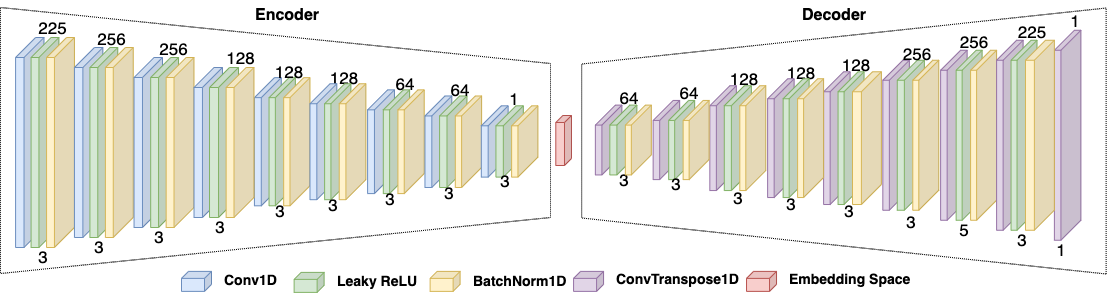
\includegraphics[width=\textwidth]{images/experiments/autoencoder_deep_1D.png}
\end{figure}

Here it can be seen, that in contrast to the one used in the initial experiment (see section \ref{sec:exp_init_experiment} figure \ref{fig:cae_2D_init}), leaky ReLU is used instead of normal ReLU. The use of the Leaky ReLU was also documented, in the work of \textit{Engel et al.} \cite{Engel2017} where it was used as activation function in the convolutional autoencoder. In the beginning for this experiment, normal ReLUs were used, but later on leaky ReLUs got applied and proven beneficial regarding model performance. This model also does not include, strides in the convolutional layers, which means, that the input does not get significantly downsampled towards the "bottleneck". One more notable difference is the depth of the network, as it has on each side 9 layers, resulting in a 18 layer network. Regarding the sublayers, also batch normalization gets applied, whereas it is also 1-dimensional, just as the convolutional layer. With all this configuration, the size of the embedding therefore would be 495x1x1. Throughout the experiment with 1D-convolutional networks, of course different configurations have been made, but this one worked out best. The results using this network can be seen later on in chapter \ref{cha:Results}.

\subsubsection{Training}
The training process for this experiment, differs in some major points from the previous ones. The main difference lies in the shape of the data. This can be concluded as here just the single frequency vectors, are used for this network and therefore the network itself has 1D-Convolutions as discussed before. Furthermore, this experiment was originally trained locally with the small subset like before, but later on access to a GPU-accelerated instance was made available. This GPU-instance, as discussed at the beginning of this chapter, enables to train complex ML-models with a large amount of data, over a long time. With this possibility, the training dataset can be utilized as this consists of several thousands of audio samples and would be too big to train locally. This does not mean, that the whole dataset was used all the time for training on this instance. With the progress of the project, several trainings with different amounts of data, could be made. Those are to be mentioned:

\begin{itemize}
    \item \textbf{Single Instrument}
    \item \textbf{Multiple Instruments (>=2)}
    \item \textbf{All Instruments}
\end{itemize}

Regarding the training performance, some interesting findings and observations could be made which get mentioned when showing the results. 

As here single frequency vectors are used, the process of creating a tensor and subsequently the dataset for the dataloader, is different. Here all spectrograms of the pre-defined and pre-processed dataset, were used, and the single frequency vectors get concatenated to form one big 3D array in the shape of amount x channels x frequency. To note the amount of channels here is also one in the input data. When experimenting with the training and its performance, also different strategies regarding shuffling got used. First on just the names of all samples got shuffled resulting in the instruments being mixed, but the frequency vectors were in the same order as in the spectrogram. This stays the same as after each epoch the data doesn't get shuffled. One more strategy that was found more successful, was also to shuffle the whole generated array, resulting in the frequency vectors of all instruments are mixed. Furthermore shuffling was also done after each epoch. The same strategies got also applied to the validation dataset, as from this point on also the validation dataset was considered. Not at least as more computational power was present from this point on. The most time, a batch-size of 32 was being used. 

Like discussed in chapter \ref{cha:Approach}, for the training also a validation step is needed. This validation was made using the validation dataset, which does not intersect with the training dataset. The validation process takes place in each epoch, after the training has been performed. This includes calculating of the train loss, back-propagating the error and optimizing the network. With this step, the network gets validated on data that has not been seen before, to prevent the network from overfitting. Introducing the validation step, also the scheduler to adapt the learning rate during the training gets applied here. Taking into account, that the network is rather complex and a huge amount of data has been used, the learning rate also has to be chosen adequately. Throughout this experiments, a small learning rate of $1e-7$ was chosen, as this led to a more stable training and better convergence. 

\subsubsection{Testing}
As described above, after each training, the current model state gets saved, those can be used for the testing and evaluation regarding synthesis. As having numerous states that got saved, the one with the lowest error score on the validation set gets taken for further steps. For the steps around testing and evaluation, the held-out test dataset gets used. This stage has been configured, to either take the whole test-dataset, a specific pitch, or a specific instrument source. By this technique its made possible to get the scores and therefore performance for certain instruments or pitch. 

\subsection{Experiments for Synthesis}
Having this kind of network that got trained on the training dataset, to reconstruct single frequency vectors, some experiments have been conducted for generating audio. As during the training the network learned how to reconstruct frequency vectors, one experiment is to examine the quality of the output for a single non-modified audio. Those are similar to the ones conducted, in first experiments above. As the main objective of this work is to examine the capability of creating novel sounds, from this point on in the project the interpolation step got introduced. With the interpolation step the encoded features in the embedded space of two instruments, get taken and value-wise interpolated. As it is known by this point, the encoder part of this network takes as input a vector of 513x1 and creates a lower-dimensional representation of it with the size of 495x1. Those representations, can be seen as the essential features, and got considered for the interpolation task. For this task, the frequency vectors of two instruments of probably the same pitch get passed through the network. Here the data does not get shuffled, as its important to produce the values in the same order as they come from the spectrograms. The output of the encoder for each instrument, gets concatenated to a 2D-array 495 x N where N is the number of encoded frequency vectors. To get a better idea of this concept, the next graphic (figure \ref{fig:exp_spec_emb_int_1D} shows two spectrograms with the corresponding output of the encoder. 

 \begin{figure}[htb!]
	\caption{Input spectrograms with embeddings and interpolated embedding}
	\label{fig:exp_spec_emb_int_1D}
	\centering
	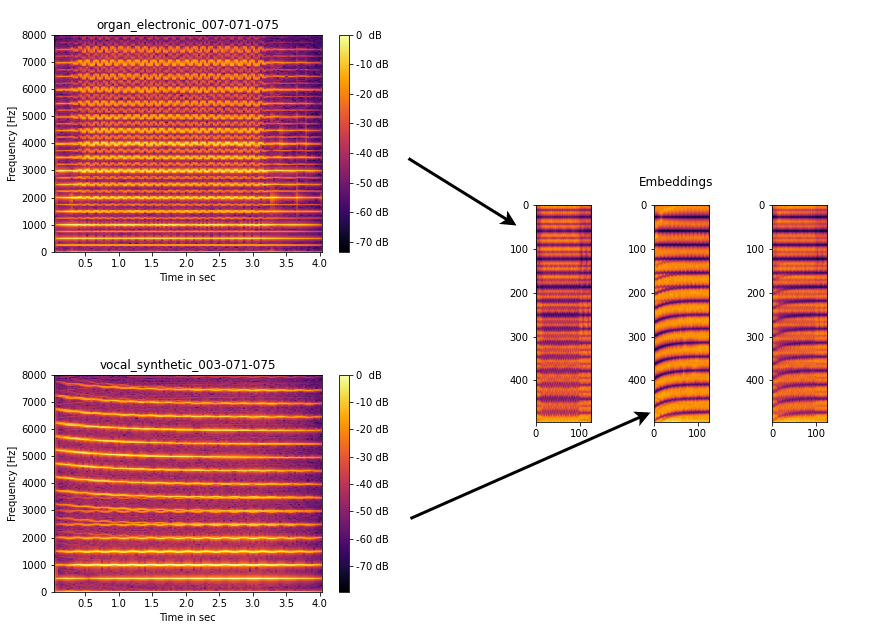
\includegraphics[width=\textwidth]{images/experiments/spec_to_emb.png}
\end{figure}

T



\section{Reconstruction with applied interpolation}

\section{Application of different models (configurations)}

\section{Measurement of results}
\chapter[Results]{Results}
\label{cha:Results}

This chapter, shows the results that could be obtained using, the experiments, mentioned in chapter \ref{cha:Experiment}. Those results contain either numbers, for assessing the model performance with a certain error performance, but also of graphics, displaying the outputs of the models. The outputs of the models, being spectrograms, will get compared with their corresponding input spectrograms. As the output of the encoder part (embedding) play a crucial role regarding audio synthesis, those also get displayed and assessed further on. Some additional graphics like signal plots Regarding the final listenable sounds, those get discussed in the next chapter.

\section{Results regarding models with single Frequency Vectors}
As described in chapter \ref{cha:Experiment} experiments have been conducted by using the single frequency vectors of the spectrograms. As a model, a 18 layer deep neural network with 1D convolutions has been trained on the reconstruction of single frequency vectors. 
Throughout the development different settings have been tried out in order to find a model with an optimal training process and performance. The amount of data on which the model has been trained on, has been varied as different performances regarding the convergence could be observed. First trainings have been made on keyboard\_synthetic mixed with guitar\_acoustic. Here it could be observed, that no sufficient convergence could be reached (MSE > 200). Training a distinct model per instrument source, showed that the instrument source has a significant influence on the convergence. For example a model trained solely on keyboard\_synthetic converged better then a model with guitar\_acoustic. Comparing the performance of a network trained on guitar\_acoustic with one trained on e.g. guitar\_electronic, showed that with the latter a better score could be reached (\textasciitilde 17). Therefore the decision was made, to combine keyboard\_synthetic and guitar\_electronic instead of acoustic, for the training. Compared to the one mixed with guitar\_acoustic a score of \textasciitilde 78 could be reached. Subsequently more instrument sources were added, until the whole training dataset was utilized. This model showed the best performance regarding its error scores and was chosen to be considered for the ongoing experiments. The next table \ref{tab:res_scores_1Dcae} shows the error scores of this model. As a short note, each trained model was chosen based on the best validation error score. 

\begin{table}[htb!]
    \centering
    \begin{tabular}{|c|c|}
        \hline
         & \textbf{MSE-Score} \\
         \hline
        \textbf{Training} & 4,237 \\
        \hline
        \textbf{Validation} & 4,638 \\
        \hline
        \textbf{Test} & 1,190 \\
        \hline
    \end{tabular}
    %\caption{MSE-Scores 1D convolutional autoencoder (8 epochs)}
    \caption{MSE-Scores 1D convolutional autoencoder}
    \label{tab:res_scores_1Dcae}
\end{table}

Here it can be seen that the error scores for training and validation are rather close, while the score on the held out test set was significantly smaller. This score could be reached with a training over 8 epochs and was considered as the best score, as after those 8 epochs the validation score increased again (despite decreasing training score). The next table \ref{tab:res_scores_1D_pitch} is also interesting as it shows, the error scores on the test set, regarding different pitches. As displaying all pitches would go beyond the scope, pitch classes from 030 to 100 have been chosen. In this case it can be seen, that all error scores have roughly the same value and do not differ significantly. Furthermore there is no visible trend if the score increases depending the pitch.

\begin{table}[htb!]
    \centering
    \begin{tabular}{|c|c|}
        \hline
         \textbf{Pitch} & \textbf{MSE-Score} \\
         \hline
         \textbf{030} & 1,049\\
         \hline
         \textbf{035} & 1,393\\
         \hline
         \textbf{040} & 0,935\\
         \hline
         \textbf{045} & 1,096\\
         \hline
         \textbf{050} & 1,019\\
         \hline
         \textbf{055} & 1,108\\
         \hline
         \textbf{060} & 1,086\\
         \hline
         \textbf{065} & 1,111\\
         \hline
         \textbf{070} & 1,164\\
         \hline
         \textbf{075} & 1,041\\
         \hline
         \textbf{080} & 1,177\\
         \hline
         \textbf{085} & 1,753\\
         \hline
         \textbf{090} & 1,100\\
         \hline
         \textbf{095} & 1,796\\
         \hline
         \textbf{100} & 2,043\\
         \hline
    \end{tabular}
    \caption{MSE-Scores for specific pitch classes using 1D convolutional autoencoder.}
    \label{tab:res_scores_1D_pitch}
\end{table}

\subsection{Experiments of single reconstruction}
Having the trained network, this one got evaluated towards the ability of reconstructing audio spectrograms and further on recreating the sounds. The next graphics (\ref{fig:res_1D_input_output}, \ref{fig:res_1D_emb} and \ref{fig:res_1D_input_output_sig}) show the result of taking a guitar sample as input and reconstructing it. 

\begin{figure}[htb!]
    \centering
    \makebox[\textwidth][c]{\begin{tabular}{@{}cc@{}}
        \makebox{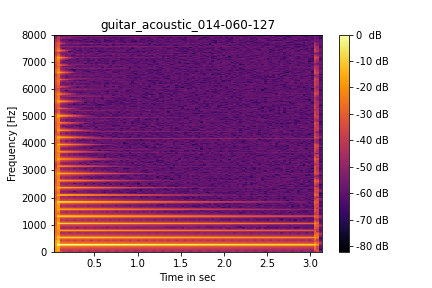
\includegraphics[width=0.55\textwidth]{images/approach/guitar_acoustic_014-060-127.png}}&
        \makebox{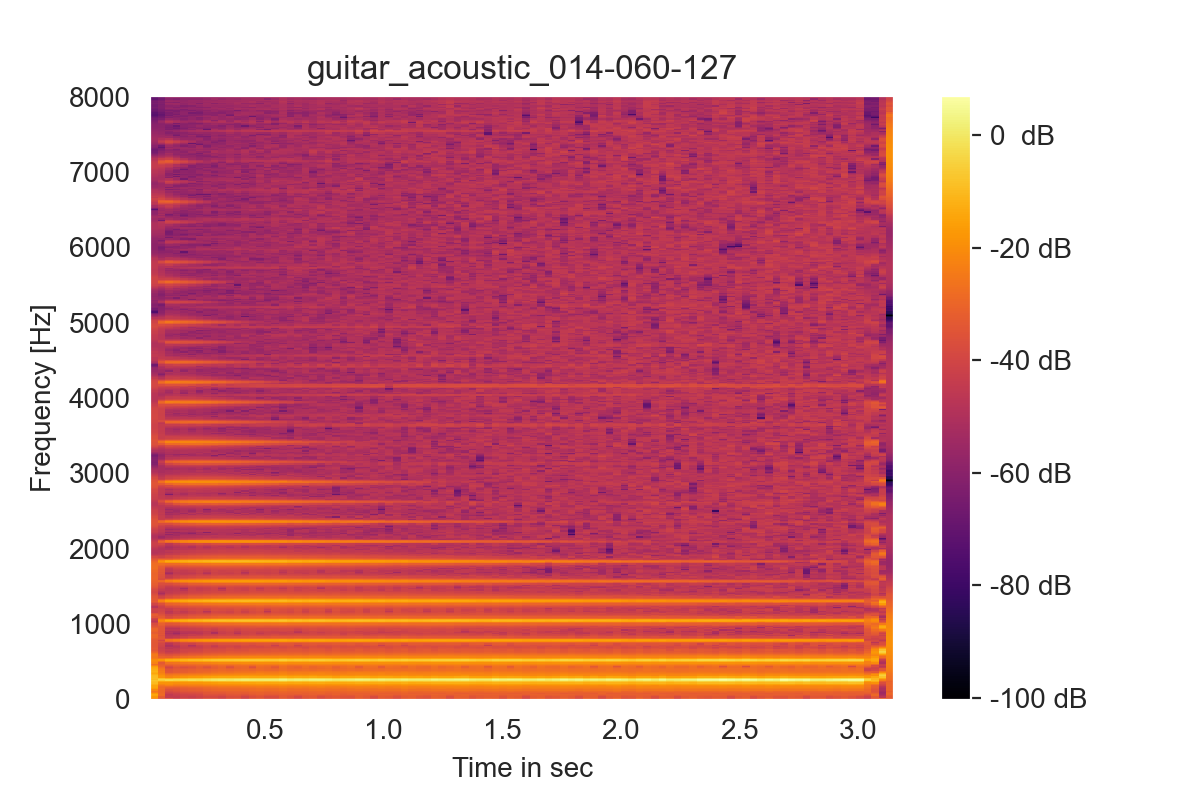
\includegraphics[width=0.55\textwidth]{images/results/rec_guitar_acoustic_014-060-127.png}}\\
        (a) & (b)
    \end{tabular}}
    \caption{input spectrogram ~(a), reconstructed spectrogram. ~(b).}
    \label{fig:res_1D_input_output}
\end{figure}

With a special look onto the reconstructability of spectrograms, figure \ref{fig:res_1D_input_output} shows the input spectrogram and the generated output spectrograms from the network. Here it can be seen, that the reconstructed spectrogram, differs in a few points from the input spectrogram. First of all it can be seen, that across the frequency areas that contain little energy in the input spectrogram, in the output more energy is present. This also means that between those areas and the sound-characteristic high energy areas, less difference is present. Furthermore regarding the original broad spectra at the beginning and at the end, those are hardly present in the output spectrogram. Knowing that these represent the stroke and the damp of the string, it can be said, that these are not present in the output. This gets also confirmed through looking at the time-domain signal.

\begin{figure}[htb!]
    \centering
    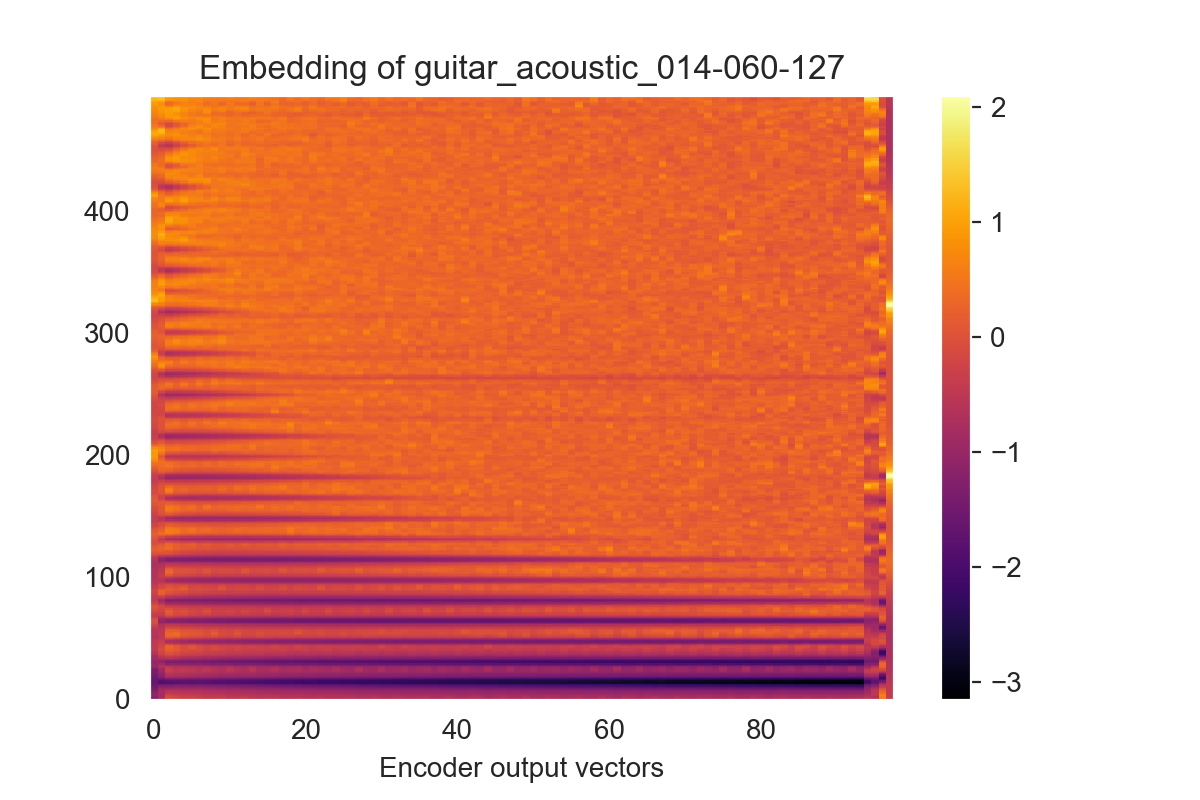
\includegraphics[width=0.55\textwidth]{images/results/emb_guitar_acoustic_014-060-127.png}
    \caption{encoding of guitar acoustic.}
    \label{fig:res_1D_emb}
\end{figure}

Looking at the graphic that depicts the embedded space, there it already can be seen that those broad spectra are not preserved. Despite of that the high energy areas (harmonics) in the input spectrogram are preserved as negative values in the embedding while the original low energy areas get represented by positive values. Also as there are no strides applied in the network, there is almost no compression in the embedding.

A final look onto the time domain plots (figure \ref{fig:res_1D_input_output_sig} also reveal, that there's no impulse at the beginning of the signal. Furthermore it also can be said, that the amplitude in general differs in its course but also in how strong it is.

\begin{figure}[htb!]
    \centering
    \makebox[\textwidth][c]{\begin{tabular}{@{}cc@{}}
        \makebox{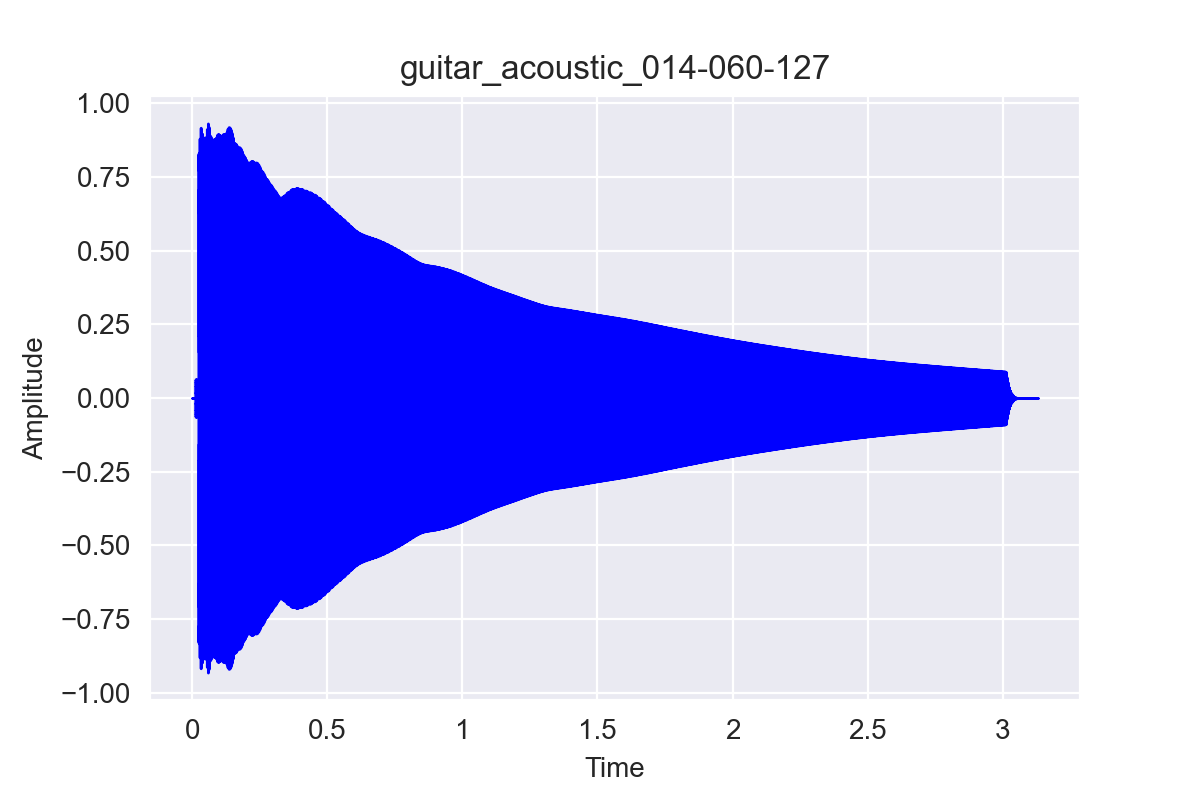
\includegraphics[width=0.55\textwidth]{images/results/inp_guitar_acoustic_014-060-127.png}}&
        \makebox{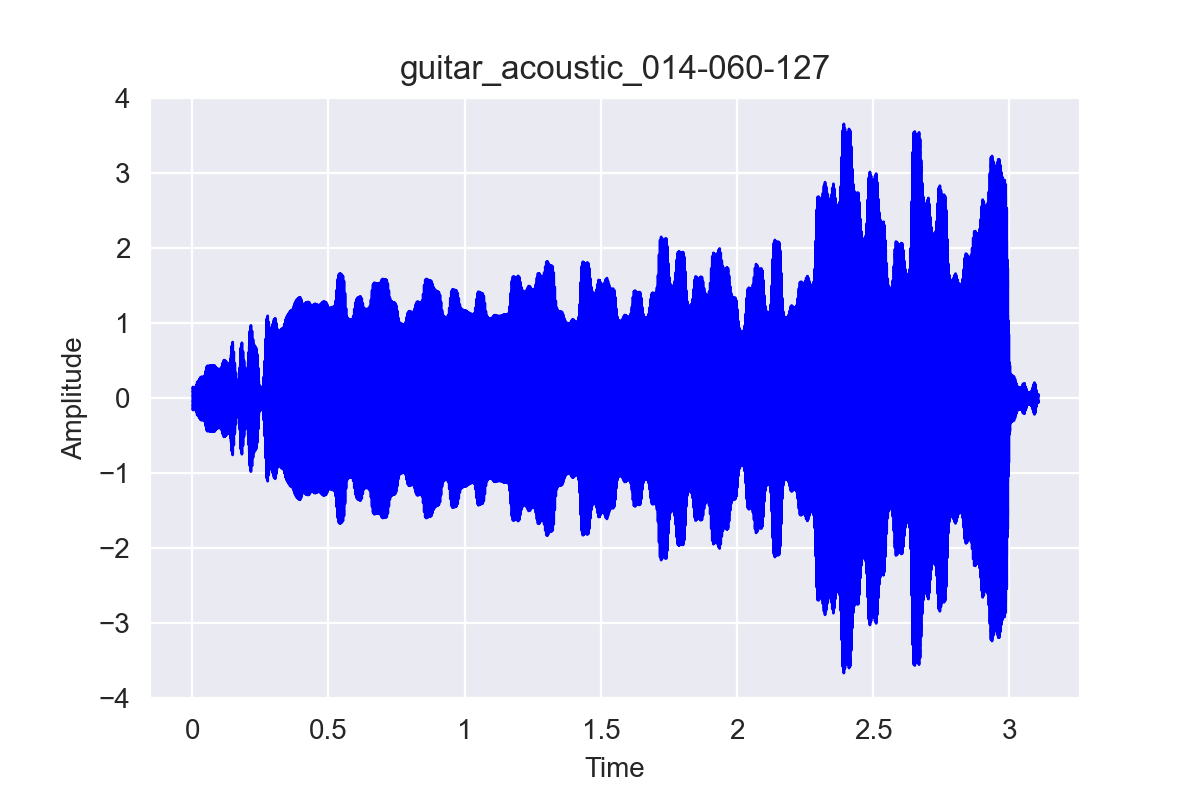
\includegraphics[width=0.55\textwidth]{images/results/out_guitar_acoustic_014-060-127.png}}\\
        (a) & (b)
    \end{tabular}}
    \caption{input signal ~(a), output signal ~(b).}
    \label{fig:res_1D_input_output_sig}
\end{figure}


\subsection{Experiments with interpolation in embedding}
With this kind of 1D convolutional autoencoder first experiments were made, that use interpolation in embedded space to synthesize novel sounds. In chapter \ref{cha:Approach} and \ref{cha:Experiment} the concept has already been described in detail. Having this concept, instrument sources were chosen, which in order got encoded and interpolated together to in order form a new embedding. The next graphic \ref{fig:res_1D_input_interpolation} shows the spectrograms of the two input instruments that were chosen to create a novel sound. For this representation an acoustic guitar and acoustic brass sample were taken and encoded. By comparing those two spectrograms, it can be seen, that they differ significantly in their structure. While it can be seen, that the guitar looses energy in its higher frequency ranges, the brass sample keeps its frequency energy over the whole time. Furthermore as the harmonics stay constant in the guitar sample, those alternate in the brass. Those properties make it interesting to use them for the interpolation and thus synthesise a novel sound. For comparative reasons, in further experiments also those two instruments have been used for the synthesis task which can be seen later on.

\begin{figure}[htb!]
    \centering
    \makebox[\textwidth][c]{\begin{tabular}{@{}cc@{}}
        \makebox{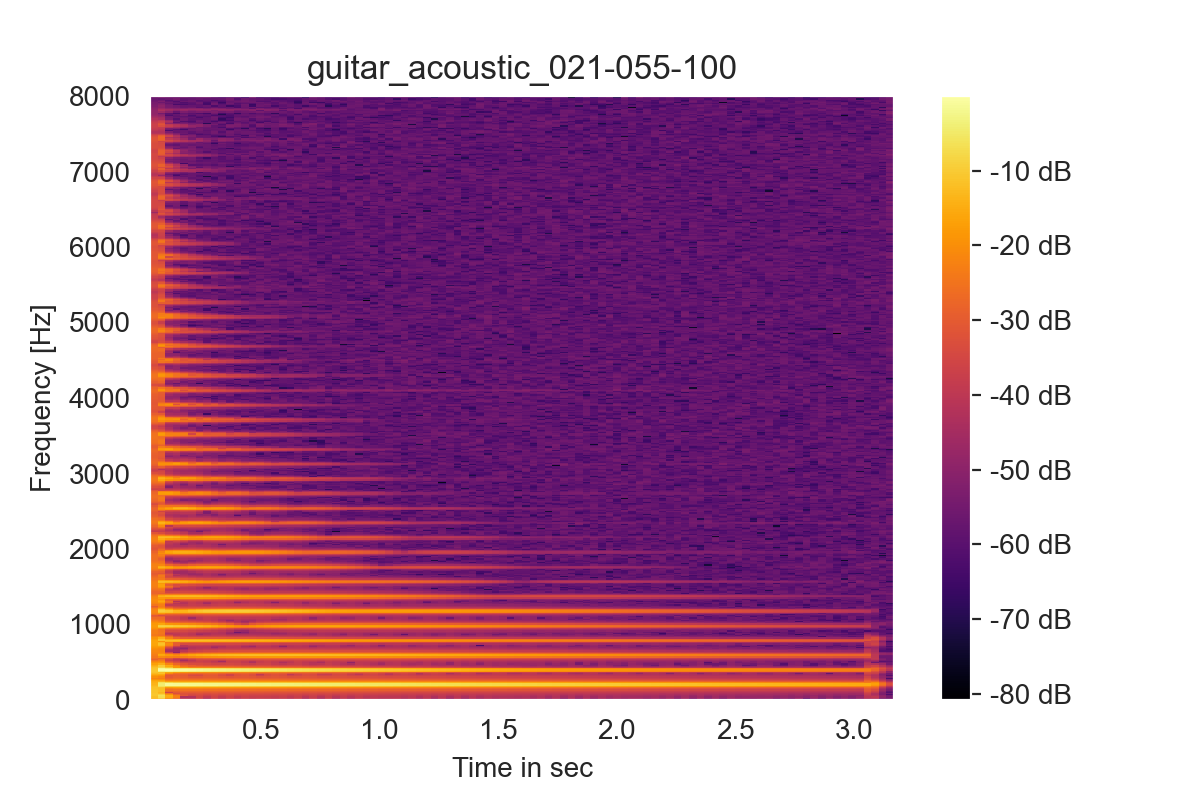
\includegraphics[width=0.55\textwidth]{images/results/guitar_acoustic_021-055-100.png}}&
        \makebox{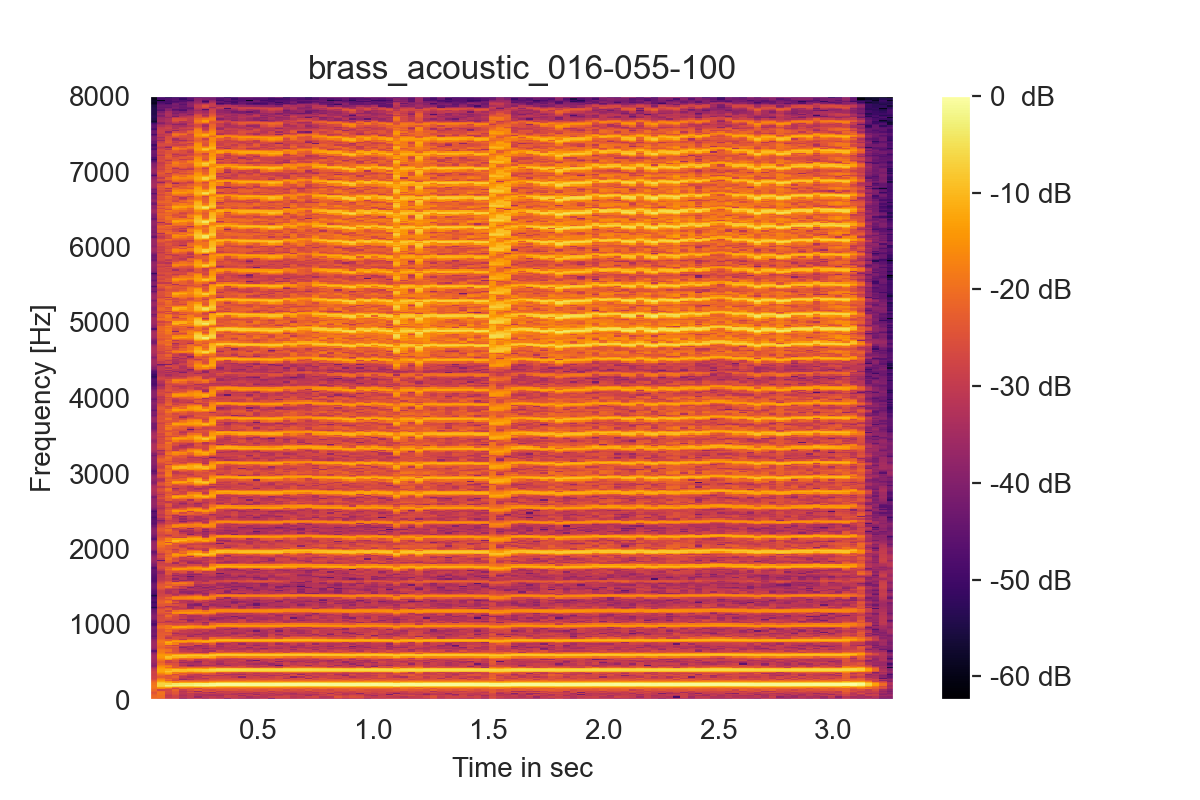
\includegraphics[width=0.55\textwidth]{images/results/brass_acoustic_016-055-100.png}}\\
        (a) & (b)
    \end{tabular}}
    \caption{guitar acoustic ~(a), brass acoustic ~(b).}
    \label{fig:res_1D_input_interpolation}
\end{figure}

After encoding, the outputs were taken and interpolated as can be seen in the next figure \ref{fig:res_1D_interpolation}a. As it can be seen, those embeddings are a compressed form of the input spectrograms. When looking onto the generated interpolated embedding, it can be said, that this one incorporates both instruments encoded features. Having this new vector, this one was fed into the decoder network to in order generate an output spectrogram that can be seen in figure \ref{fig:res_1D_interpolation}b. 

\begin{figure}[htb!]
    \centering
    \makebox[\textwidth][c]{\begin{tabular}{@{}cc@{}}
        \makebox{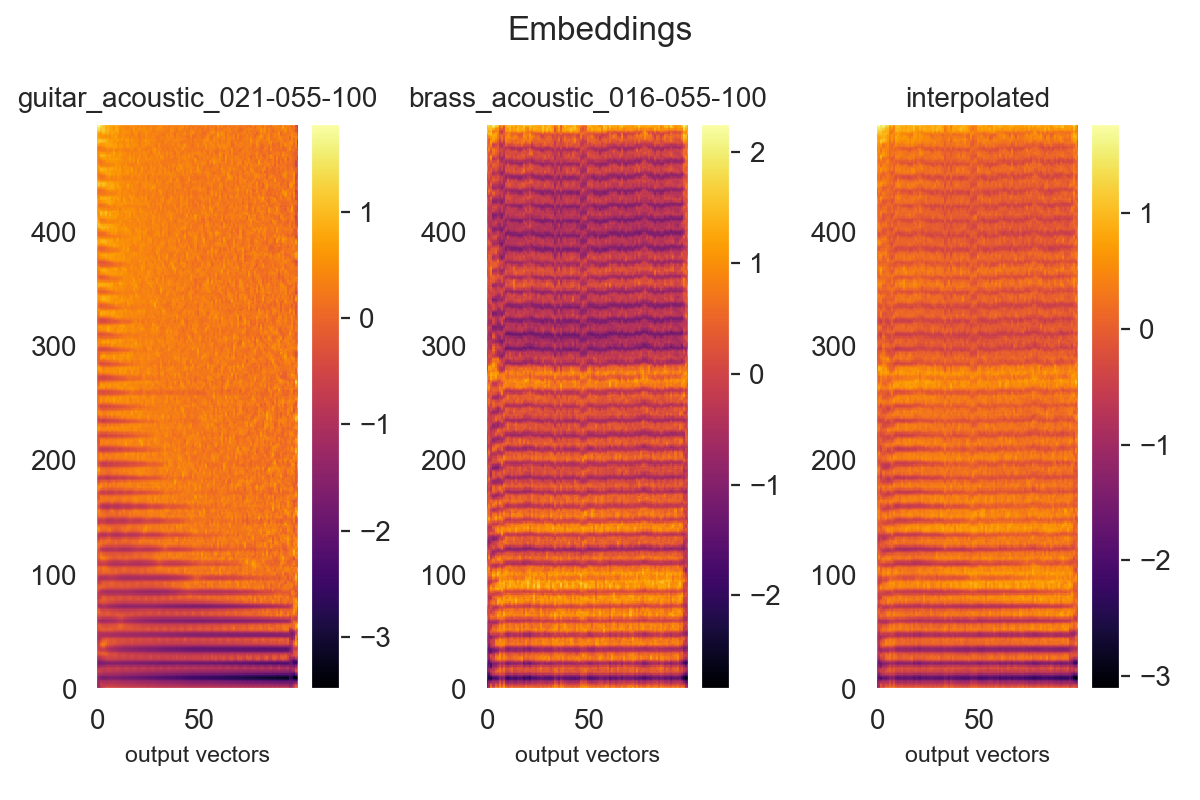
\includegraphics[width=0.55\textwidth]{images/results/interp_emb_guitar_acoustic_021-055-100&brass_acoustic_016-055-100.png}}&
        \makebox{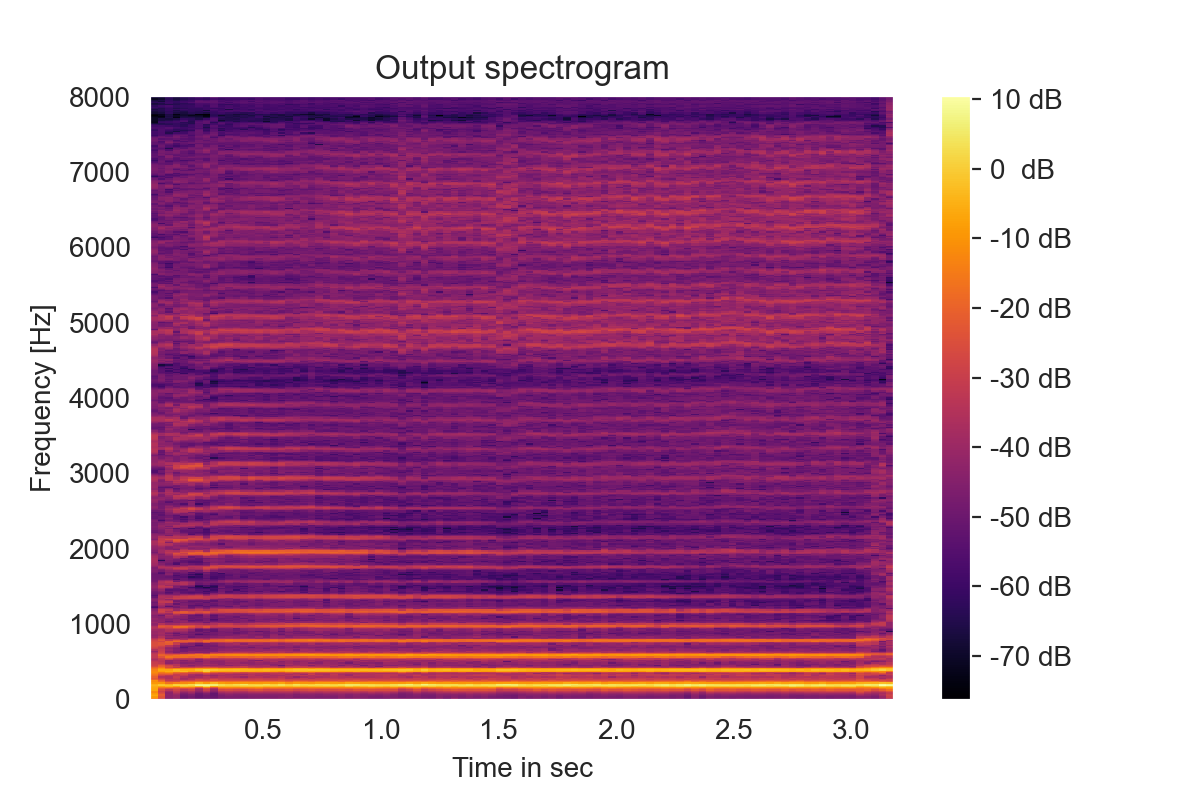
\includegraphics[width=0.55\textwidth]{images/results/guitar_acoustic_021-055-100&brass_acoustic_016-055-100_output_spec.png}}\\
        (a) & (b)
    \end{tabular}}
    \caption{embedding interpolation ~(a), output signal ~(b).}
    \label{fig:res_1D_interpolation}
\end{figure}

Having the final spectrogram here as output, it can be seen, that spectral data of both input spectrograms are basicaly contained. Similar to the output spectrogram in figure \ref{fig:res_1D_input_output}b this one also does not contain the impulse (guitar stroke) at the beginning. To finally obtain a listenable sound, the output spectrogram has to get converted back to time-domain, which in this case gets done with the Griffin-Lim algorithm \cite{Griffin1984} as no phase information is present. 

To improve the quality of the output but also to examine the performance of other types of networks some further experiments have been made using 2D convolutions but also additional post-processing steps.

\section{Results of experiments with spectrogram frames}
The here shown results, correspond to the described experiments in section \ref{sec:exp_spec_slice}. Here again a 2D convolutional autoencoder has been utilized to (re)synthesize audio. As input data for the neural networks, overlapping spectrograms snippets with the length of 3 along the time axis have been considered. In contrast to the previous network, this was supposed to bring better results, regarding the output but especially to preserve transients. As different networks with different stridings (compression) were trained and used, the results should also show the differences in the output but also in their quality regarding audio (re)synthesis. Additionally the encoded data gets examined by calculating the correlation coefficients between samples (mostly of the same pitch). By that it can be seen how much the encodings of different instruments differ. Additionally it also can be examined how good the different networks extract the essential features of the input data. Throughout the project these correlation coefficients got depicted in a so-called correlation matrix. Displaying one here would would not work out sufficiently, as because of its many values, those are hardly readable without zooming in. Because of this, just the findings get discussed later on in chapter Discussion. Finally also additional post-processing steps get applied, which help to correct the energy and thus the quality of the output. The results shown here are without energy correction, but the effect will also be discussed later on in the discussion.

The following table \ref{tab:res_scores_2Dcae} shows the MSE error scores of the different 2D convolutional networks. As mentioned in chapter \ref{cha:Experiment}, three networks were trained, that differ in their configuration regarding striding and thus have different embedding sizes. These networks therefore are called single, double- and triple stride networks, regarding the amount of striding on each network side. By this they can be distinguished better in this work. In table \ref{tab:res_scores_2Dcae} it can be seen that by using a different amount of strides, this has a an impact onto the score. The network with just one stride on each side, has the lowest error whereas the networks with two or three strides have a significant higher error. Regarding the difference between training, validation and testing error all three networks show the same behaviour as the validation error is higher then the training error with the test score being the best. 

\begin{table}[htb!]
    \centering
    \captionsetup{justification=centering}
    \begin{tabular}{|c|c|c|c|}
        \hline
         & \textbf{single-stride} & \textbf{double-stride} & \textbf{triple-stride} \\
         \hline
        \textbf{Training} & 9,779 & 13,717 & 18,292 \\
        \hline
        \textbf{Validation} & 10,094 & 14,056 & 19,056 \\
        \hline
        \textbf{Test} & 7,826 & 10,708 & 16,655 \\
        \hline
    \end{tabular}
    \caption{MSE-Scores 2D convolutional autoencoder - single stride, double stride, triple stride.}
    %\caption{MSE-Scores 2D convolutional autoencoder - single stride (9 epochs), double stride (8 epochs), triple stride (16 epochs).}
    \label{tab:res_scores_2Dcae}
\end{table}

Compared to the error score of the 1D convolutional network, it can be said, that all error scores are significantly higher. In case of this work, the score does not mean, that the quality of the output is worse, especially regarding the final output sound. The latter will get discussed later on in the discussion of this work

As during the previous experiment also the scores regarding different pitches were calculated, the next table \ref{tab:res_scores_2D_pitch} shows the different scores regarding pitches ranging from 30 to 100. Similar to the 1D convolutional network, the error scores regarding the pitch do not show a specific trend. Interestingly the scores of the triple-strided network has some rather strong outliers regarding samples around the classes 045-050. Having the same error scores this also does not mean, that all pitches have the same audible quality but more on that in chapter \ref{cha:Discussion}. 


\begin{table}[htb!]
    \centering
    \begin{tabular}{|c|c|c|c|}
        \hline
         \textbf{Pitch} & \textbf{single-stride} & \textbf{double-stride} & \textbf{triple-stride}\\
         \hline
         \textbf{030} & 7,084 & 9,175 & 12,241\\
         \hline
         \textbf{035} & 7,912 & 12,294 & 15,426\\
         \hline
         \textbf{040} & 7,292 & 11,205 & 18,639\\
         \hline
         \textbf{045} & 7,251 & 12,434 & 22,151\\
         \hline
         \textbf{050} & 6,840 & 9,903 & 20,287\\
         \hline
         \textbf{055} & 7,535 & 10,434 & 18,102\\
         \hline
         \textbf{060} & 7,444 & 10,128 & 17,670\\
         \hline
         \textbf{065} & 8,313 & 10,286 & 16,497\\
         \hline
         \textbf{070} & 7,410 & 9,868 & 14,894\\
         \hline
         \textbf{075} & 7,850 & 9,949 & 14,273\\
         \hline
         \textbf{080} & 8,624 & 10,529 & 15,486\\
         \hline
         \textbf{085} & 9,299 & 11,090 & 16,598\\
         \hline
         \textbf{090} & 8,798 & 11,435 & 16,415\\
         \hline
         \textbf{095} & 9,948 & 12,032 & 17,049\\
         \hline
         \textbf{100} & 12,346 & 13,179 & 19,812\\
         \hline
    \end{tabular}
    \caption{MSE-Scores for specific pitch classes using 2D convolutional autoencoder.}
    \label{tab:res_scores_2D_pitch}
\end{table}

\subsection{Experiments of single reconstruction}
Having mentioned the error scores regarding reconstructing spectral audio data, those cannot be taken solely to assess the performance of the network. Therefore experiments, like with the previous network, were conducted in recreating single spectrograms. With those the ability towards reconstructing audio spectrograms becomes assessed visually and auditorily for the purpose of audio (re)synthesis.
For comparative reasons, the same spectrogram source has been chosen like with the previous network. As the original input spectrogram has already been shown in figure \ref{fig:res_1D_input_output}a, here just the output of the encoder part (embedding) but also the total output gets depicted (see figures \ref{fig:res_single_str_2D_output_emb}, \ref{fig:res_double_str_2D_output_emb} and \ref{fig:res_triple_str_2D_output_emb}). The spectrograms in each of these graphics were generated with single-, double- and triple-stride networks and do not contain the energy correcting post-processing mechanism. Despite of this fact, it can be seen when looking onto all the output spectrograms (\ref{fig:res_single_str_2D_output_emb}a, \ref{fig:res_double_str_2D_output_emb}a and \ref{fig:res_triple_str_2D_output_emb}a), that all preserve the broad spectra at the beginning and ending of the spectrograms, especially by looking onto the first one. When comparing again the low energy areas of the input spectrogram, to the output spectrograms, it can be said, that they also contain similar little energy. Again it can also be seen, that the embedding looks like a spectrogram but in a compressed form of the input, as it also contains similar structures. Contrary to the embedding in figure \ref{fig:res_1D_emb} the high energy areas have positive numbers while original low energy area have negative numbers.

\begin{figure}[htb!]
    \centering
    \captionsetup{justification=centering}
    \makebox[\textwidth][c]{\begin{tabular}{@{}cc@{}}
        \makebox{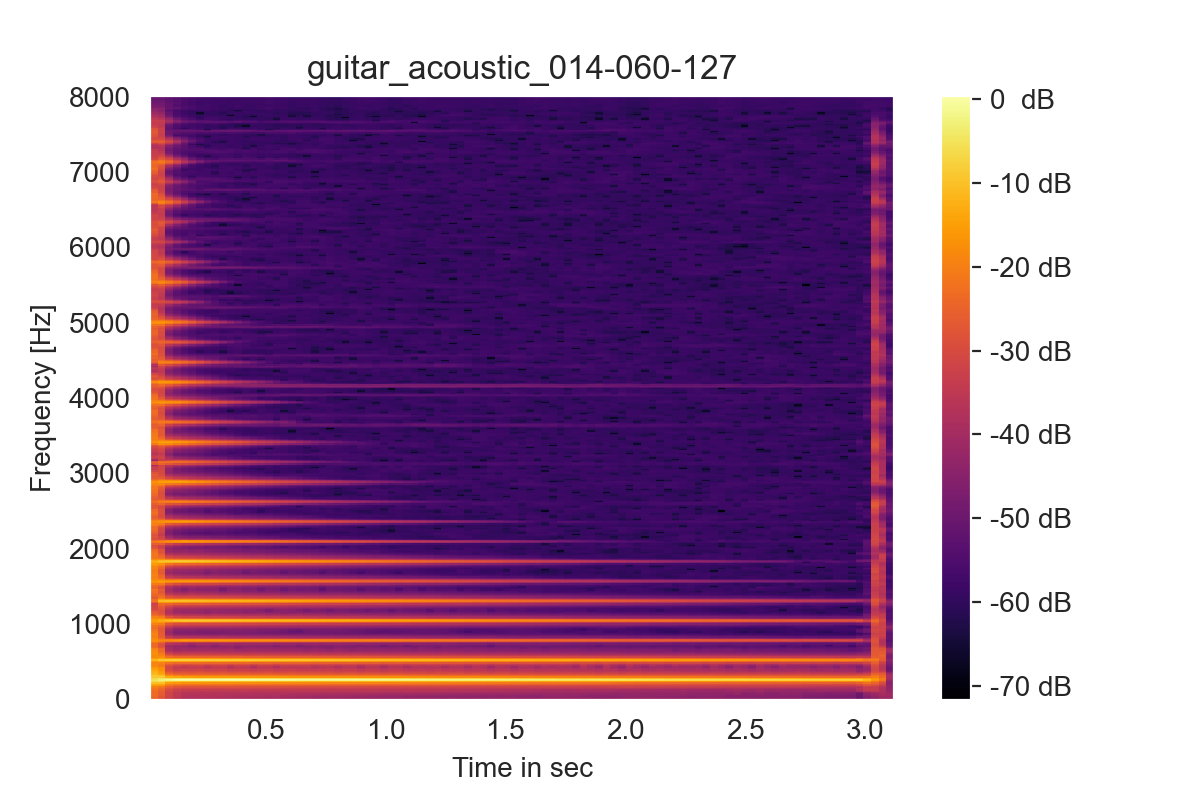
\includegraphics[width=0.55\textwidth]{images/results/single_str/out_guitar_acoustic_014-060-127.png}}&
        \makebox{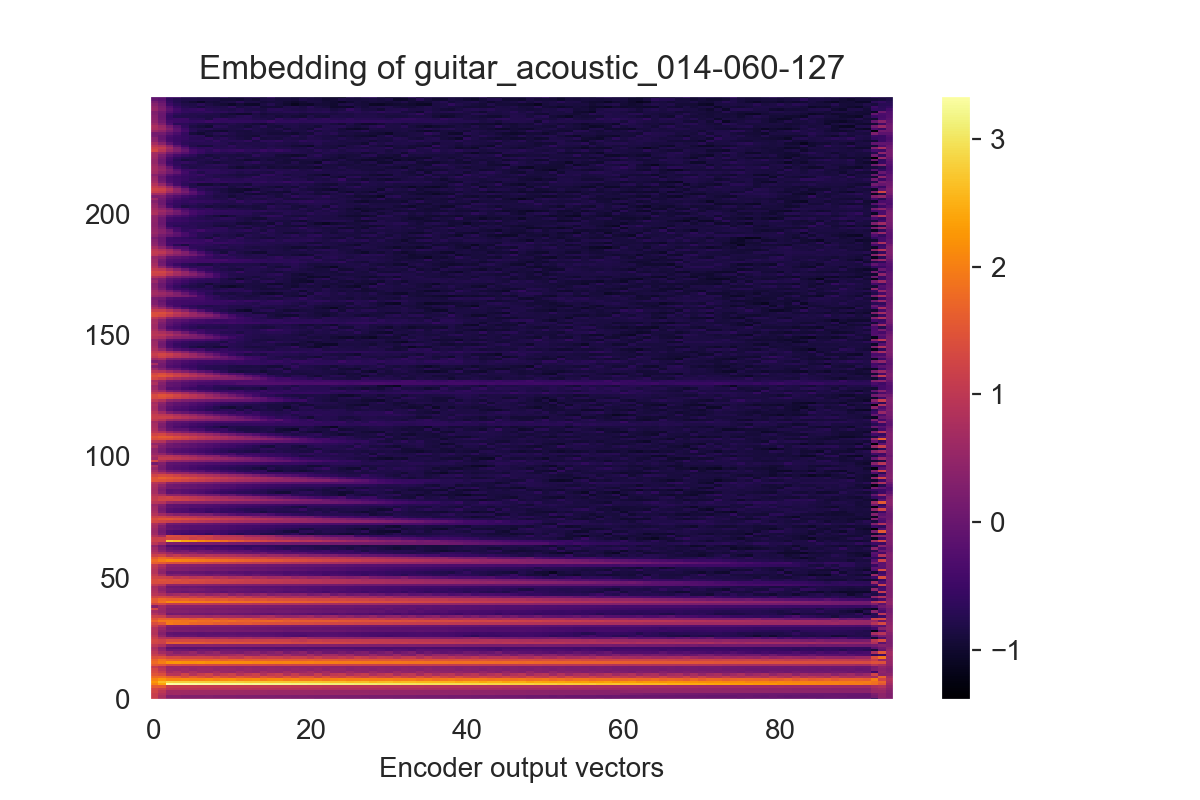
\includegraphics[width=0.55\textwidth]{images/results/single_str/emb_guitar_acoustic_014-060-127.png}}\\
        (a) & (b)
    \end{tabular}}
    \caption{reconstruction of guitar acoustic ~(a), embedding of guitar acoustic ~(b)\\single stride model.}
    \label{fig:res_single_str_2D_output_emb}
\end{figure}

With a look on the output of the double-stride network (figure \ref{fig:res_double_str_2D_output_emb}a), it also can be said, that the broad spectra are preserved but with less energy. This can be also noticed when looking on the output spectrogram of the triple stride network (figure \ref{fig:res_triple_str_2D_output_emb}). The latter also shows less energy in the high energy areas and less "precise harmonics" (washed out). 

\begin{figure}[htb!]
    \centering
    \captionsetup{justification=centering}
    \makebox[\textwidth][c]{\begin{tabular}{@{}cc@{}}
        \makebox{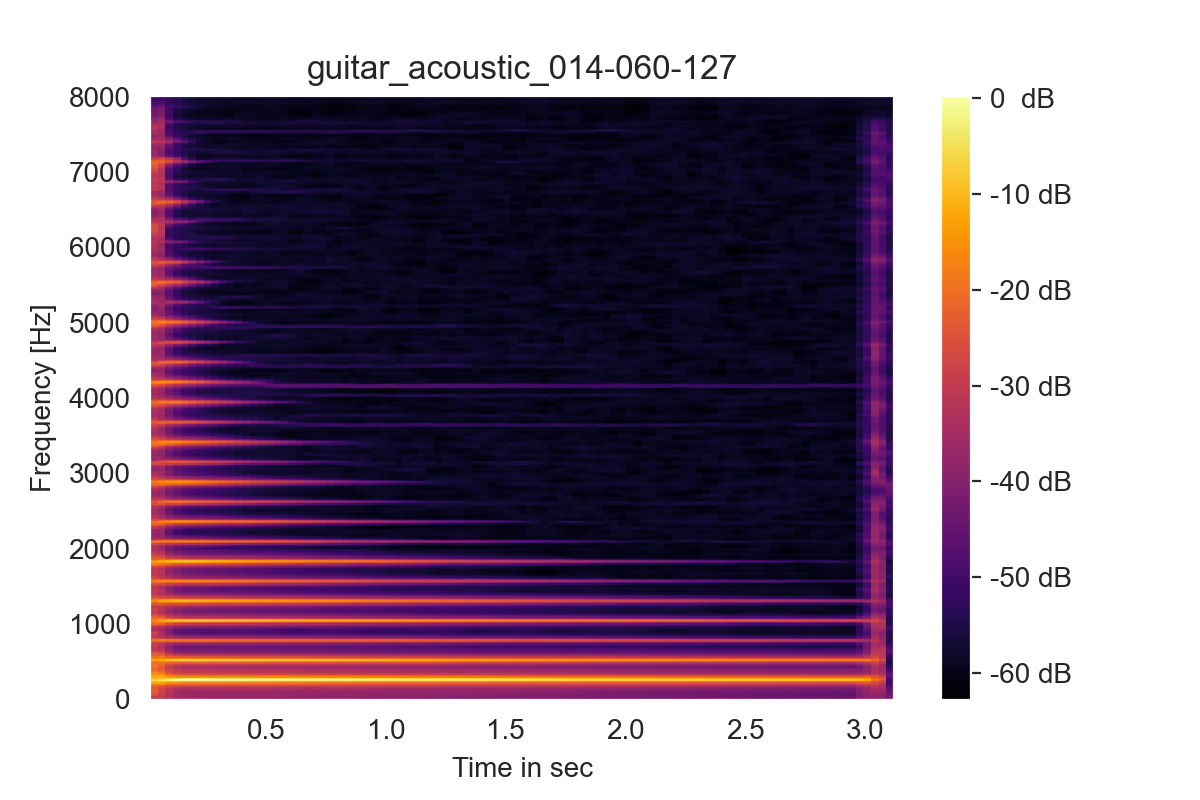
\includegraphics[width=0.55\textwidth]{images/results/double_str/guitar_acoustic_014-060-127.png}}&
        \makebox{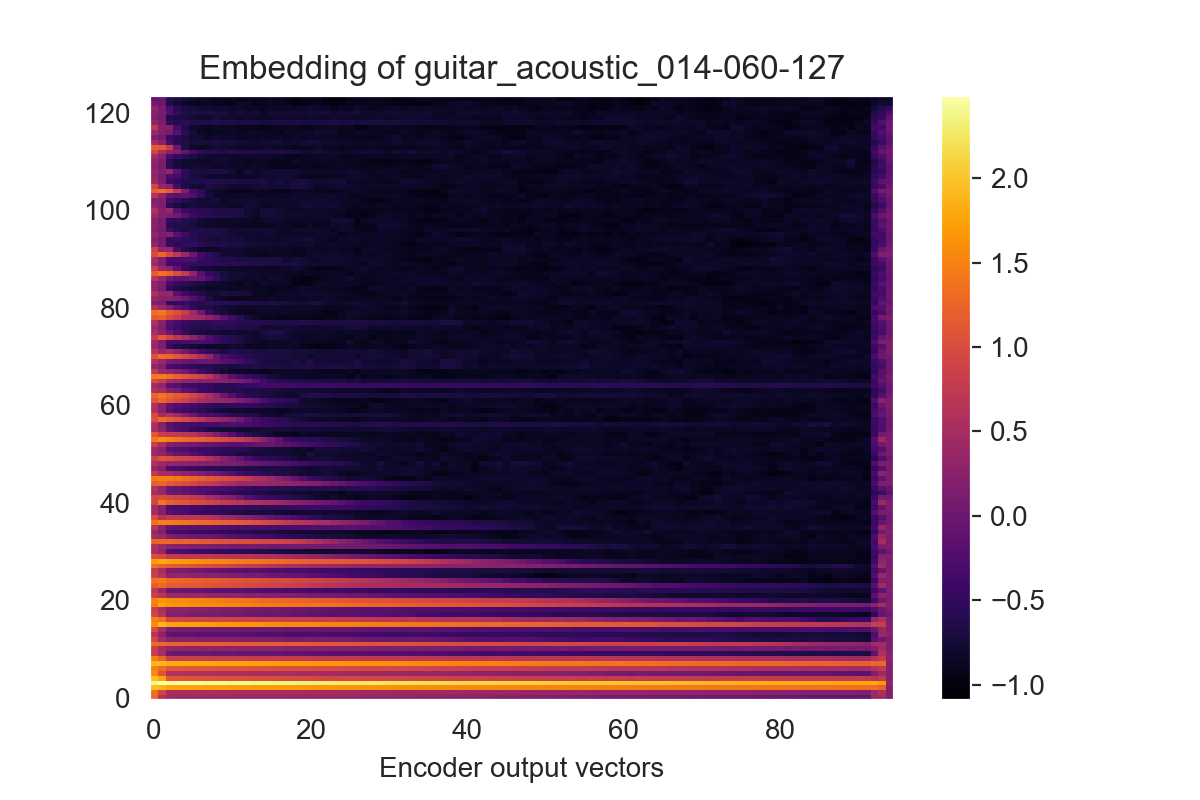
\includegraphics[width=0.55\textwidth]{images/results/double_str/emb_guitar_acoustic_014-060-127.png}}\\
        (a) & (b)
    \end{tabular}}
    \caption{reconstruction of guitar acoustic ~(a), embedding of guitar acoustic ~(b)\\double stride model.}
    \label{fig:res_double_str_2D_output_emb}
\end{figure}

Looking onto the embeddings of the two networks it can be said, that those contain signifcantly less values across the y-axis. Comparing it to the input but also the output, despite of the significant compression, the significant harmonic features and general structures are present as positive numbers (regarding the colorscale). As concerning the double strided network, the embedding still has a fine granularity contrary to the one obtained by the triple strided network.

\begin{figure}[htb!]
    \centering
    \captionsetup{justification=centering}
    \makebox[\textwidth][c]{\begin{tabular}{@{}cc@{}}
        \makebox{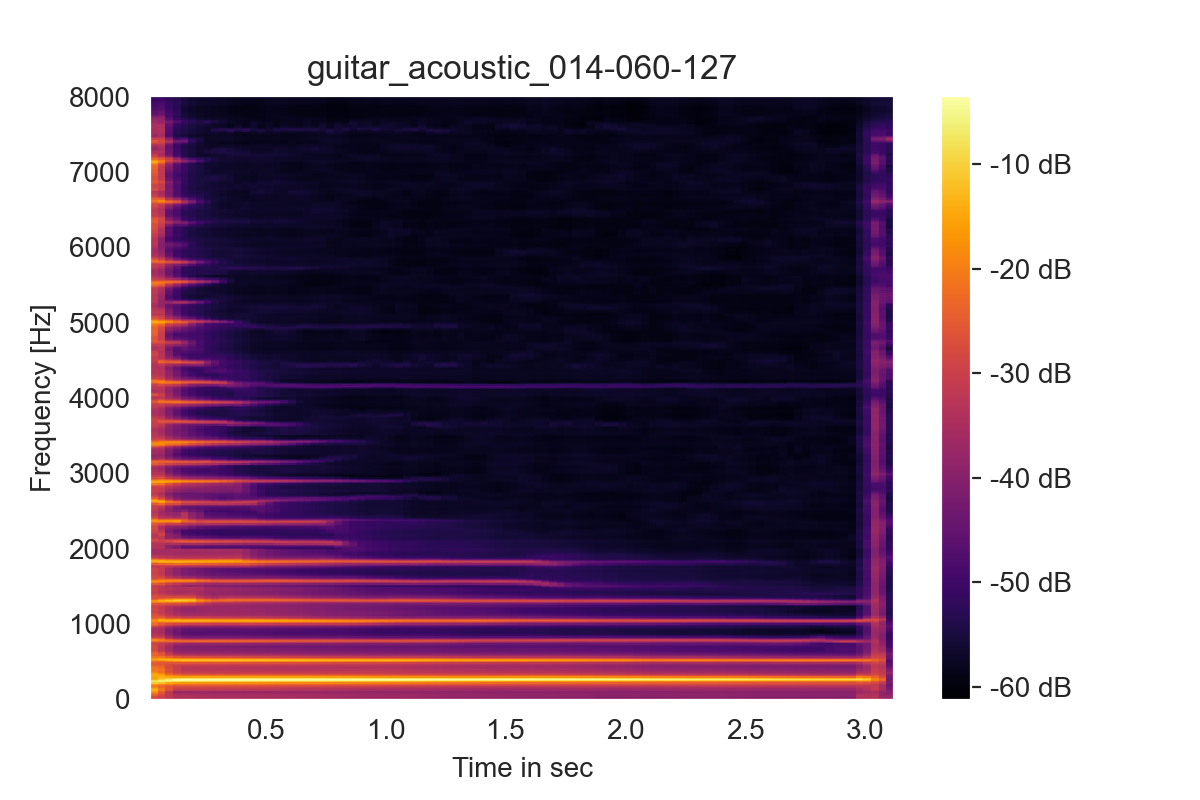
\includegraphics[width=0.55\textwidth]{images/results/triple_str/guitar_acoustic_014-060-127.png}}&
        \makebox{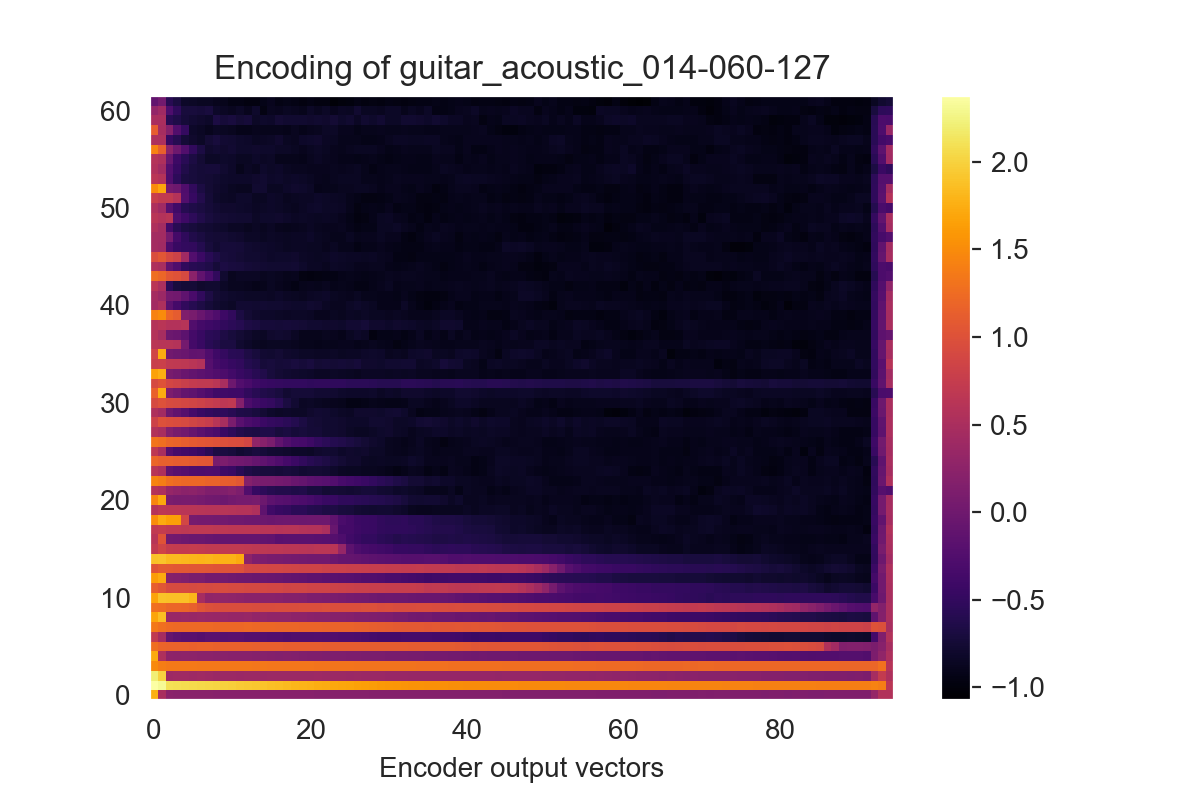
\includegraphics[width=0.55\textwidth]{images/results/triple_str/emb_guitar_acoustic_014-060-127.png}}\\
        (a) & (b)
    \end{tabular}}
    \caption{reconstruction of guitar acoustic ~(a), embedding of guitar acoustic ~(b)\\triple stride model.}
    \label{fig:res_triple_str_2D_output_emb}
\end{figure}

\subsection{Experiments with interpolation in embedding}
The results in this section show the resulting outputspectrograms, that got generated by interpolation of the embedding space vectors. This has already been done with the 1D convolutional network where novel sounds could be generated. As with the 2D convolutional networks used in this experiment, promising results in reconstructing single spectrograms could be obtained, this experiments yield interesting results. Not at least, as the embedding got more compressed, this also effects synthesizing new audio, as this is done by interpolating the embeddings. The following graphics (\ref{fig:res_single_str_2D_inter_output}, \ref{fig:res_double_str_2D_inter_output} and \ref{fig:res_triple_str_2D_inter_output} show again the interpolation between the same two instrumental sources, for comparative reasons. Again also the resulting output spectrograms are displayed to see the final result. The audititory quality again gets assessed and discussed in the next chapter.
When looking at the embeddings in the three graphics, that after interpolating, the features of both instruments are visible in the result. Here it can be seen that the "harmonic" features of the brass sample do not fade contrary to the guitar samples. Nevertheless because of the interpolation the features are present but having lower values as it interpolates mostly between negative and positive numbers.  The areas where the both samples have common features (lower harmonics), rather stay equally valued as those have close values in both embeddings. 

\begin{figure}[htb!]
    \centering
    \makebox[\textwidth][c]{\begin{tabular}{@{}cc@{}}
        \makebox{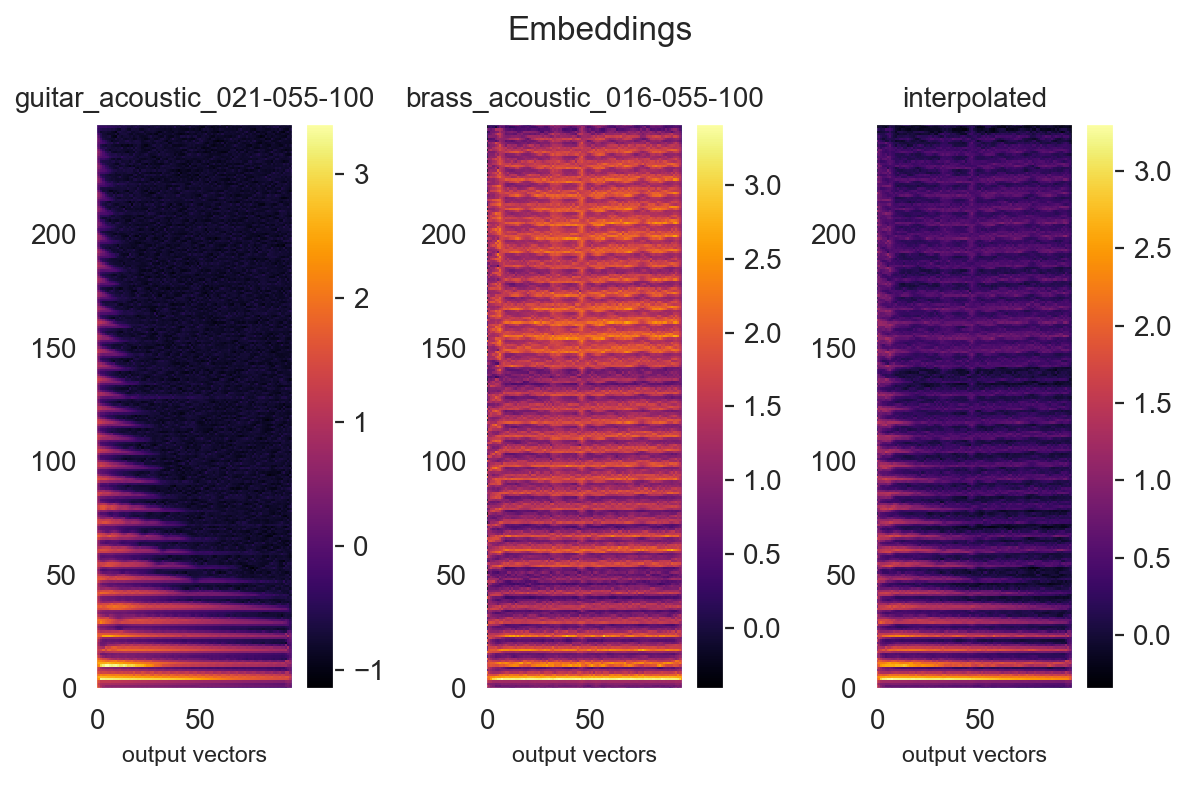
\includegraphics[width=0.55\textwidth]{images/results/single_str/inter_guitar_acoustic_021-055-100&brass_acoustic_016-055-100_original_0.5.png}}&
        \makebox{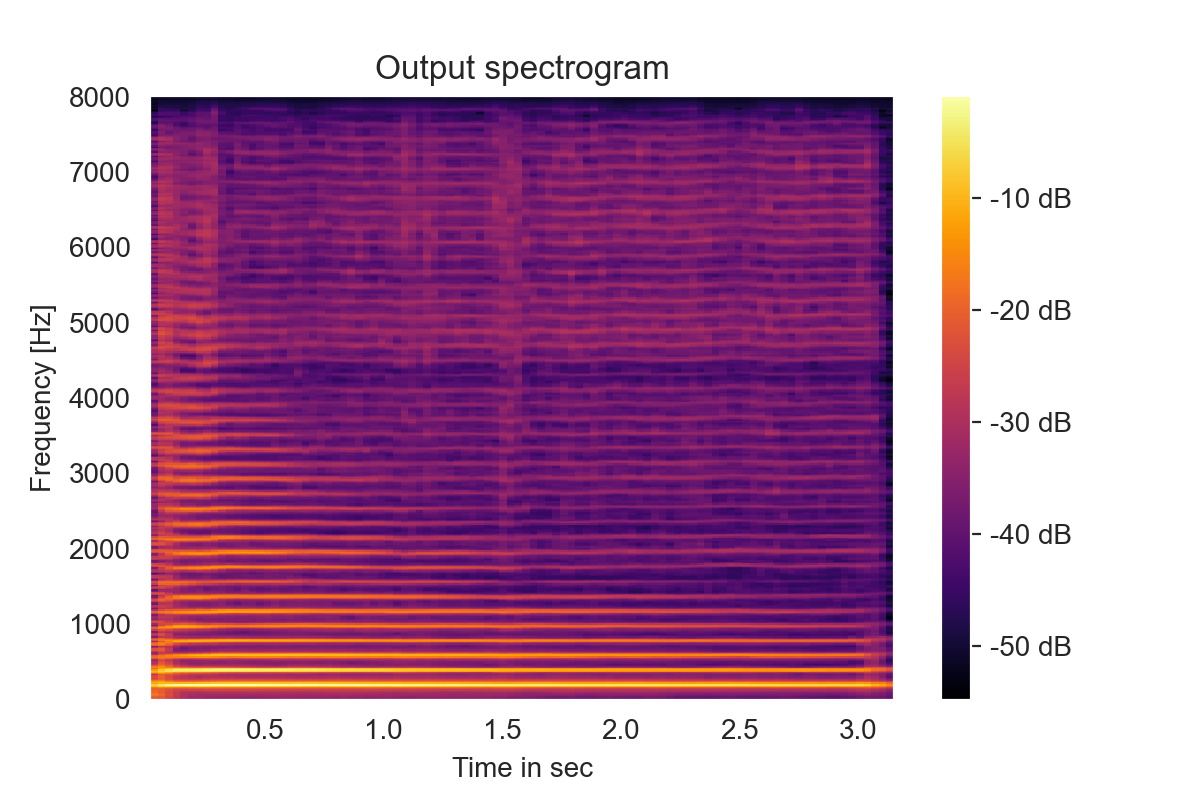
\includegraphics[width=0.55\textwidth]{images/results/single_str/guitar_acoustic_021-055-100&brass_acoustic_016-055-100_output_0.5.png}}\\
        (a) & (b)
    \end{tabular}}
    \caption{embedding interpolation ~(a), output signal ~(b).}
    \label{fig:res_single_str_2D_inter_output}
\end{figure}

By looking again on the decoded output it can be seen, that again both instruments are present. Compared to the result in the first experiments, the guitar sample is more present with these kind of network. Contrary to the experiment with single sample reconstruction, here the difference between the different strided networks, can be noticed even more. With special notice to the higher harmonics of the original brass samples. Those harmonics appear more precise with the single strided network (see figure \ref{fig:res_single_str_2D_inter_output}b). In the output of the double-stride network in figure \ref{fig:res_double_str_2D_inter_output}b the "contours" coming from the brass sample, are less sharp then with the single stride.

\begin{figure}[htb!]
    \centering
    \makebox[\textwidth][c]{\begin{tabular}{@{}cc@{}}
        \makebox{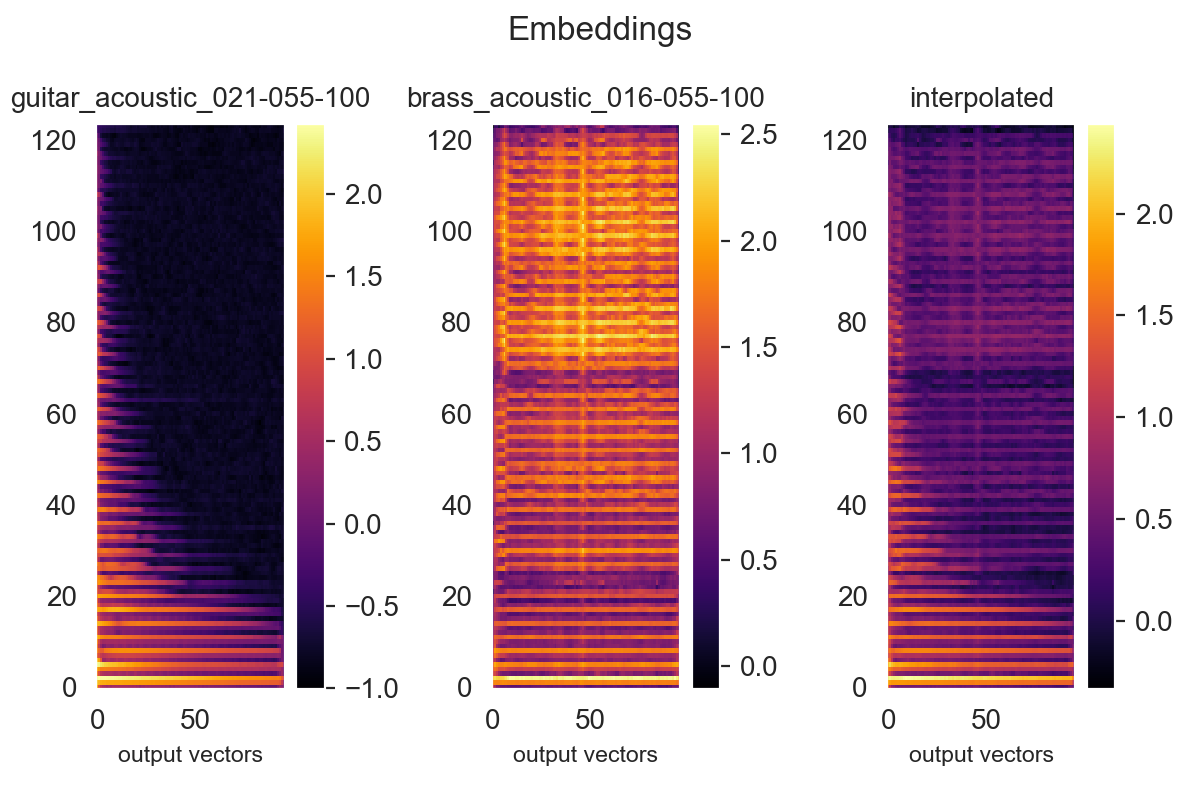
\includegraphics[width=0.55\textwidth]{images/results/double_str/inter_guitar_acoustic_021-055-100&brass_acoustic_016-055-100_original_0.5.png}}&
        \makebox{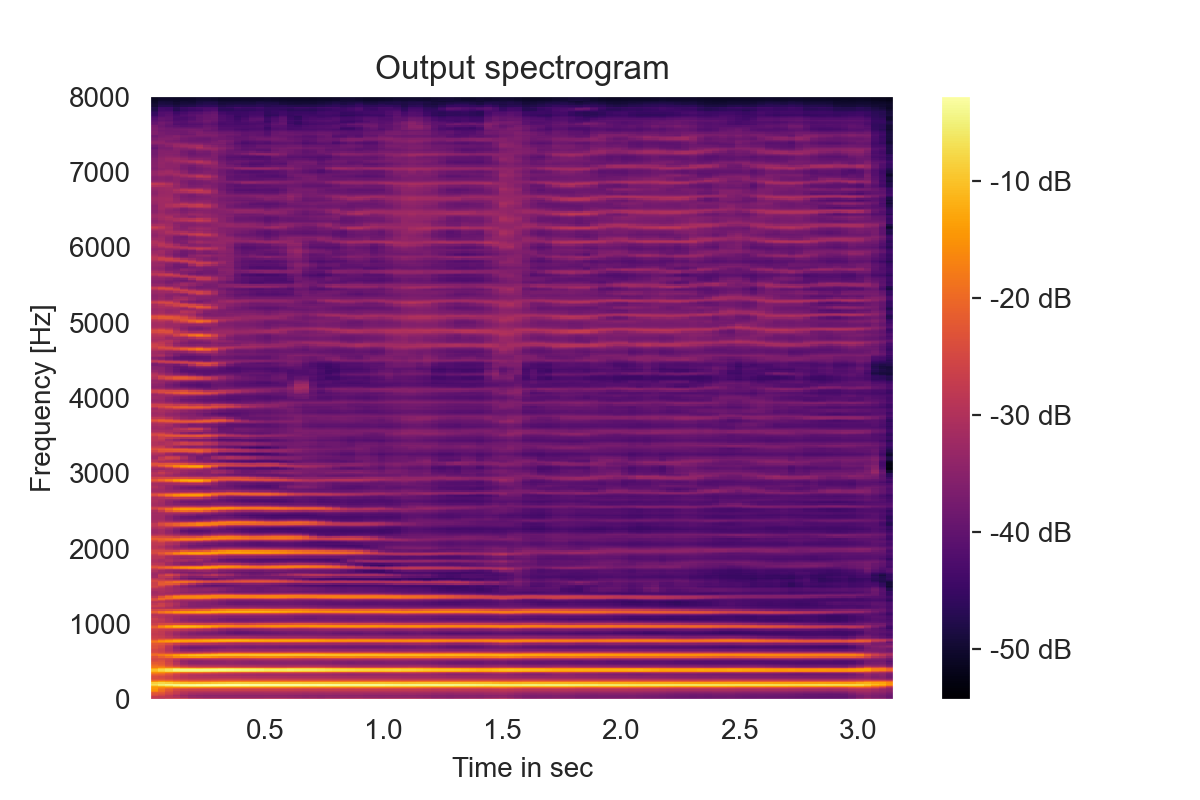
\includegraphics[width=0.55\textwidth]{images/results/double_str/guitar_acoustic_021-055-100&brass_acoustic_016-055-100_output_0.5.png}}\\
        (a) & (b)
    \end{tabular}}
    \caption{embedding interpolation ~(a), output signal ~(b).}
    \label{fig:res_double_str_2D_inter_output}
\end{figure}

Taking the output of the triple strided network (figure \ref{fig:res_triple_str_2D_inter_output}) into account, the difference to the other networks can be seen clearly. The encoded features, again contain the same structure as the input spectrograms, but due to the three-fold striding, just the most significant information is present. Comparing the interpolated embeddings it also can be said that in the latter, the guitar features can be recognized better. Looking at the final output spectrogram in \ref{fig:res_triple_str_2D_inter_output}b it can be seen, that the original fine harmonics aren't present anymore. The energy values of the different frequencies over time don't remain constant and show "washed out" contours. Also the fine changes over time are not as precisely present as with previous network configurations. Nevertheless both instrumental features can be recognized in the final output. 

\begin{figure}[htb!]
    \centering
    \makebox[\textwidth][c]{\begin{tabular}{@{}cc@{}}
        \makebox{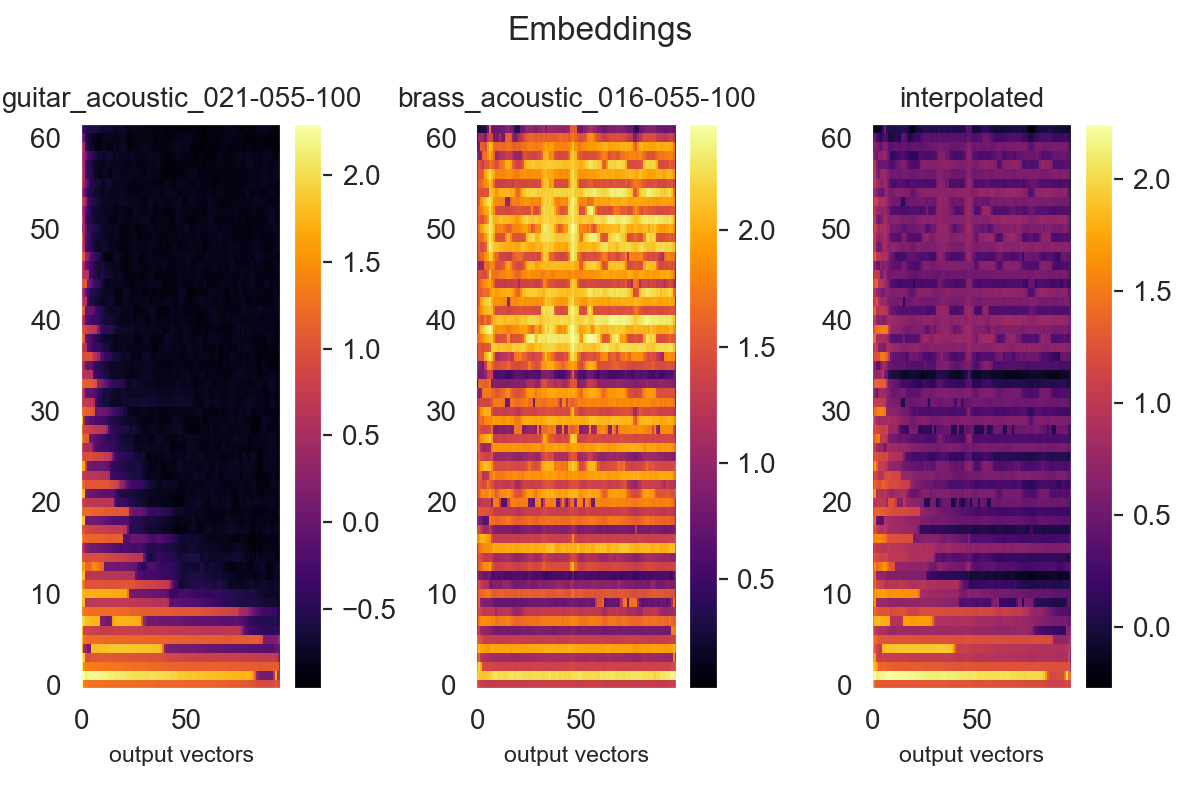
\includegraphics[width=0.55\textwidth]{images/results/triple_str/inter_guitar_acoustic_021-055-100&brass_acoustic_016-055-100_original_0.5.png}}&
        \makebox{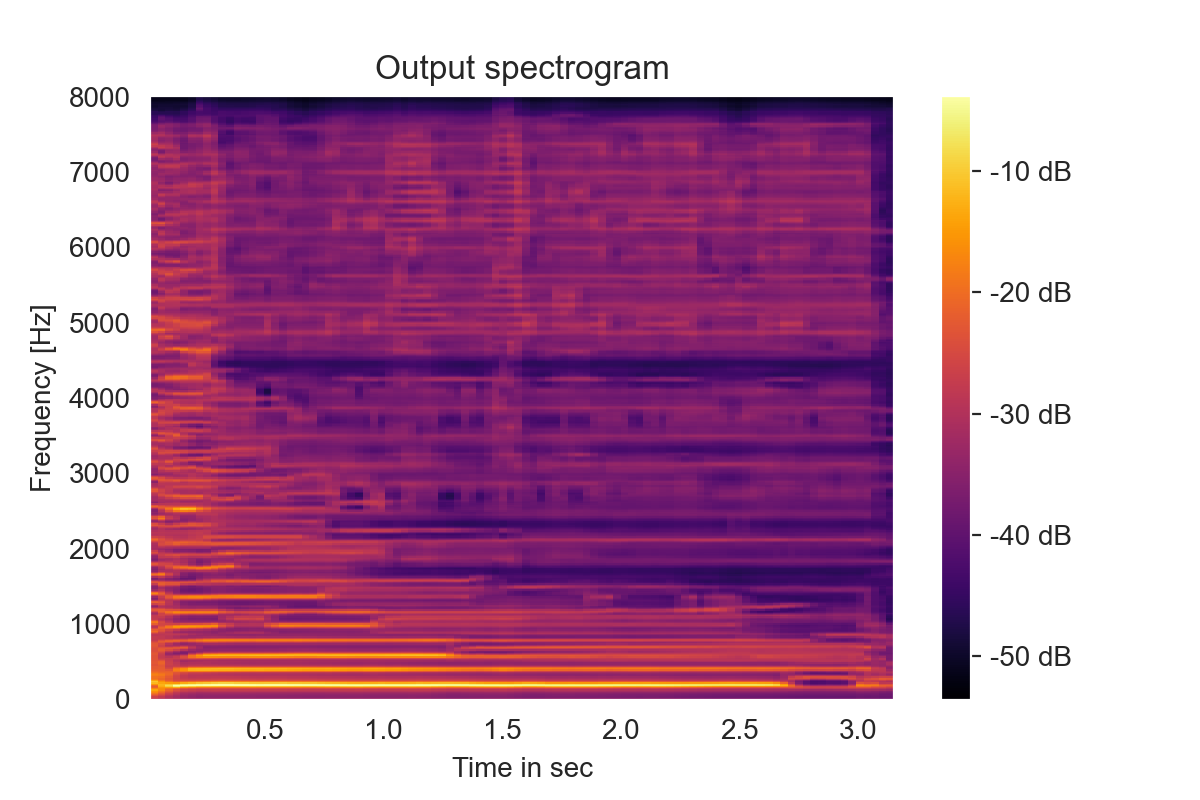
\includegraphics[width=0.55\textwidth]{images/results/triple_str/guitar_acoustic_021-055-100&brass_acoustic_016-055-100_output_0.5.png}}\\
        (a) & (b)
    \end{tabular}}
    \caption{embedding interpolation ~(a), output signal ~(b)}
    \label{fig:res_triple_str_2D_inter_output}
\end{figure}

Again in the discussion part, the auditive quality of all outputs presented here, with and without energy correction, gets assessed and brought into relation with the here displayed spectrograms.

\section{Results with mel-spectrograms}

The final experiments are again done with a 2D convolutional network, but using mel-scale spectrograms instead of log-magnitude. In chapter \ref{cha:Experiment} under section \ref{sec:exp_mel} an introduction to the mel-scale has been given. As those log-mel spectrograms are a compressed version of the log-magnitude spectrograms and emphasizes the lower frequencies, these experiments are expected to bring different but interesting results. This is again meant regarding the model performance but also towards the quality of reconstructing spectrograms with or without modification of the embeddings. The results again get depicted in tables filled with the MSE scores of training, validation and testing but also the scores regarding specific pitch classes of the test set. Later on again the graphics contain the output spectrograms and embeddings with and without interpolation. Again three different networks with single, double and triple strides were used. Those are similar in their structure to the ones used with log-magnitude spectrograms, which was already explained in the previous chapter.

The following table \ref{tab:res_scores_2D_mel} shows the training, validation and testing scores of all three different networks. First of all the MSE scores of all networks are significantly, higher than the ones of the log-magnitude networks. An exception makes the testing score of the single-stride network as it is equally to the training score of the triple-strided log-magnitude network. The scores between the networks, also increase with the amount of compression, making the single-stride network again the best performing network regarding its score. Interestingly the validation score of the single-stride network, is the only one that is higher as its corresponding training score. The double- and triple-stride networks therefore show that they have a lower score on reconstructing unseen data. Again the auditory quality will get assessed in the next chapter \ref{cha:Discussion}.

\begin{table}[htb!]
    \centering
    \captionsetup{justification=centering}
    \begin{tabular}{|c|c|c|c|}
        \hline
         & \textbf{single-stride} & \textbf{double-stride} & \textbf{triple-stride} \\
         \hline
        \textbf{Training} & 30,579 & 49,685 & 62,833 \\
        \hline
        \textbf{Validation} & 31,084 & 48,439 & 60,471\\
        \hline
        \textbf{Test} & 18,322 & 33,689 & 43,300\\
        \hline
    \end{tabular}
    \caption{MSE-Scores 2D convolutional autoencoder with log-mel spectrograms - single stride, double stride, triple stride}
    % \caption{MSE-Scores 2D convolutional autoencoder - mel-scale - single stride (15 epochs), double stride (21 epochs), triple stride (68 epochs)}
    \label{tab:res_scores_2D_mel}
\end{table}

Like in the previous experiments, the network performance has been evaluated towards certain pitch classes. The following table \ref{tab:res_scores_2D_pitch_mel} shows the MSE scores of different pitch classes. For comparative reasons, again they got categorized on a scale from 30 to 100 in 5 steps. Contrary to those scores in the previous experiments, here the values show, that the lower pitched samples have the best score. With some exceptions/outliers, the error scores increase with a clear trend, the higher pitched the used samples were. Interestingly the difference in the score, between the highest and lowest used samples, increases, the more compression is used. 

\begin{table}[htb!]
\centering
\begin{tabular}{|c|c|c|c|}
\hline
\textbf{pitch} & \textbf{single-stride} & \textbf{double-stride} & \textbf{triple-stride} \\ \hline
\textbf{030}   & 17,178                 & 24,567                 & 30,302                 \\ \hline
\textbf{035}   & 18,380                 & 26,142                 & 36,509                 \\ \hline
\textbf{040}   & 19,382                 & 34,125                 & 44,062                 \\ \hline
\textbf{045}   & 22,036                 & 55,770                 & 51,097                 \\ \hline
\textbf{050}   & 22,398                 & 41,101                 & 49,810                 \\ \hline
\textbf{055}   & 22,159                 & 43,215                 & 56,664                 \\ \hline
\textbf{060}   & 21,472                 & 40,493                 & 54,690                 \\ \hline
\textbf{065}   & 22,303                 & 40,140                 & 51,926                 \\ \hline
\textbf{070}   & 23,875                 & 41,950                 & 50,904                 \\ \hline
\textbf{075}   & 24,571                 & 37,424                 & 49,297                 \\ \hline
\textbf{080}   & 29,053                 & 43,572                 & 60,926                 \\ \hline
\textbf{085}   & 29,395                 & 46,822                 & 62,750                 \\ \hline
\textbf{090}   & 33,316                 & 51,408                 & 72,206                 \\ \hline
\textbf{095}   & 31,385                 & 51,593                 & 70,607                 \\ \hline
\textbf{100}   & 32,129                 & 51,426                 & 70,890                 \\ \hline
\end{tabular}
\caption{MSE-Scores for specific pitch classes using 2D convolutional autoencoder using mel-scale.}
\label{tab:res_scores_2D_pitch_mel}
\end{table}

\subsection{Experiments of single reconstruction}
Similar to the other experiments to assess the ability of reconstructing spectrograms and therefore recreate audio samples, in this section the embeddings and corresponding output spectrograms are depicted. There again the properties and respective differences to the other experiments get assessed. Regarding the auditory quality the results get discussed in chapter \ref{cha:Discussion}. The here shown results again correspond just to the reconstruction of single samples without interpolation. As in these last experiments the mel-scale as different scale was used, the corresponding input spectrograms are shown in advance. Figure \ref{fig:res_2D_mel_guit} shows the input spectrogram of the single reconstruction experiments.

\begin{figure}[htb!]
    \centering
    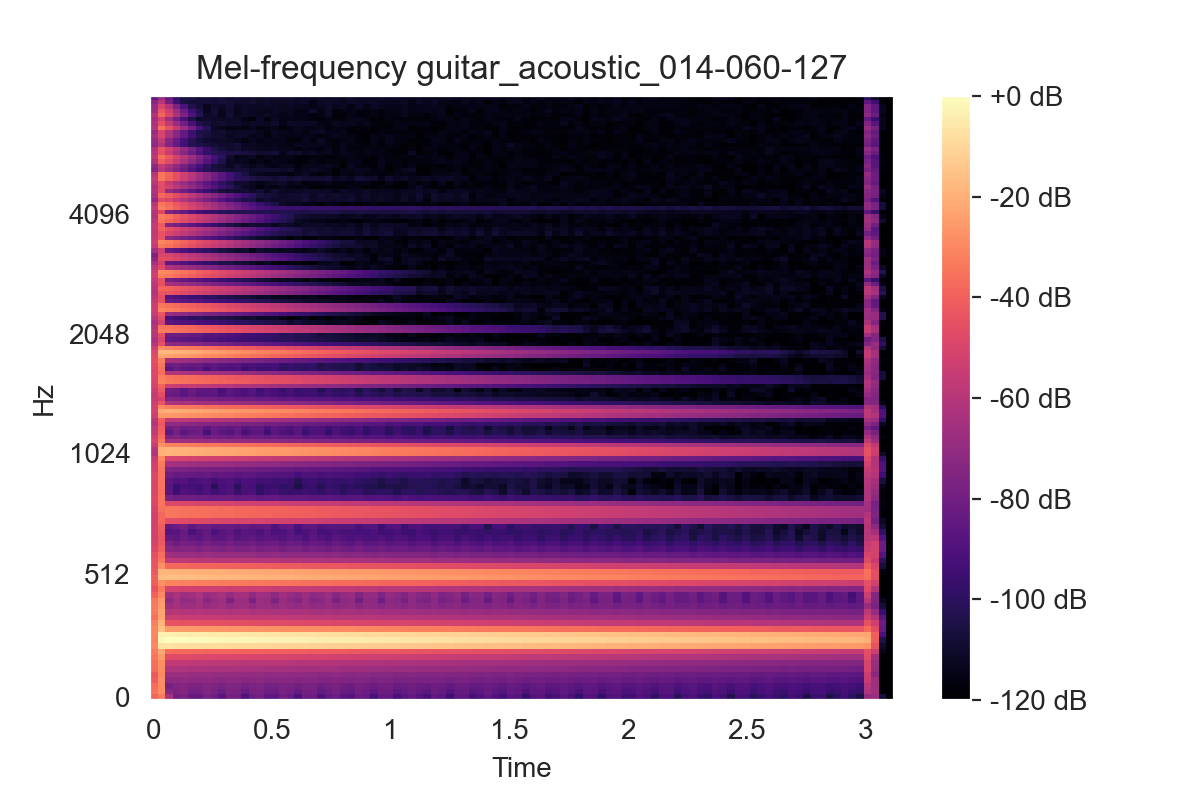
\includegraphics[width=0.55\textwidth]{images/results/mel_guitar_acoustic_014-060-127.png}
    \caption{original mel-spectrogram of guitar acoustic.}
    \label{fig:res_2D_mel_guit}
\end{figure}

The next three figures (\ref{fig:res_mel_single_str_2D_output_emb}, \ref{fig:res_mel_double_str_2D_output_emb} and \ref{fig:res_mel_triple_str_2D_output_emb}) show the output spectrograms but also the embeddings of the guitar sample depicted in figure \ref{fig:res_2D_mel_guit}. As its known at this point, the mel-spectrograms are already a compressed version log-magnitude spectrograms, as they contain 128 values instead 513. Thus it can be seen on the y-axis of the embeddings, that those embeddings are even more compressed than in the last experiment (size of 56, 28 and 14). Furthermore it can be noticed regarding the embeddings of the first two networks (figures \ref{fig:res_mel_single_str_2D_output_emb}b and \ref{fig:res_mel_double_str_2D_output_emb}b), that contrary to the previous experiments with log-magnitde spectrograms, the low energy areas are positive valued. The high-energy areas and harmonics are therefore negative valued. Concerning the scale it can be also said that those embeddings have a narrower value range then those in the previous experiments. 

\begin{figure}[htb!]
    \centering
    \captionsetup{justification=centering}
    \makebox[\textwidth][c]{\begin{tabular}{@{}cc@{}}
        \makebox{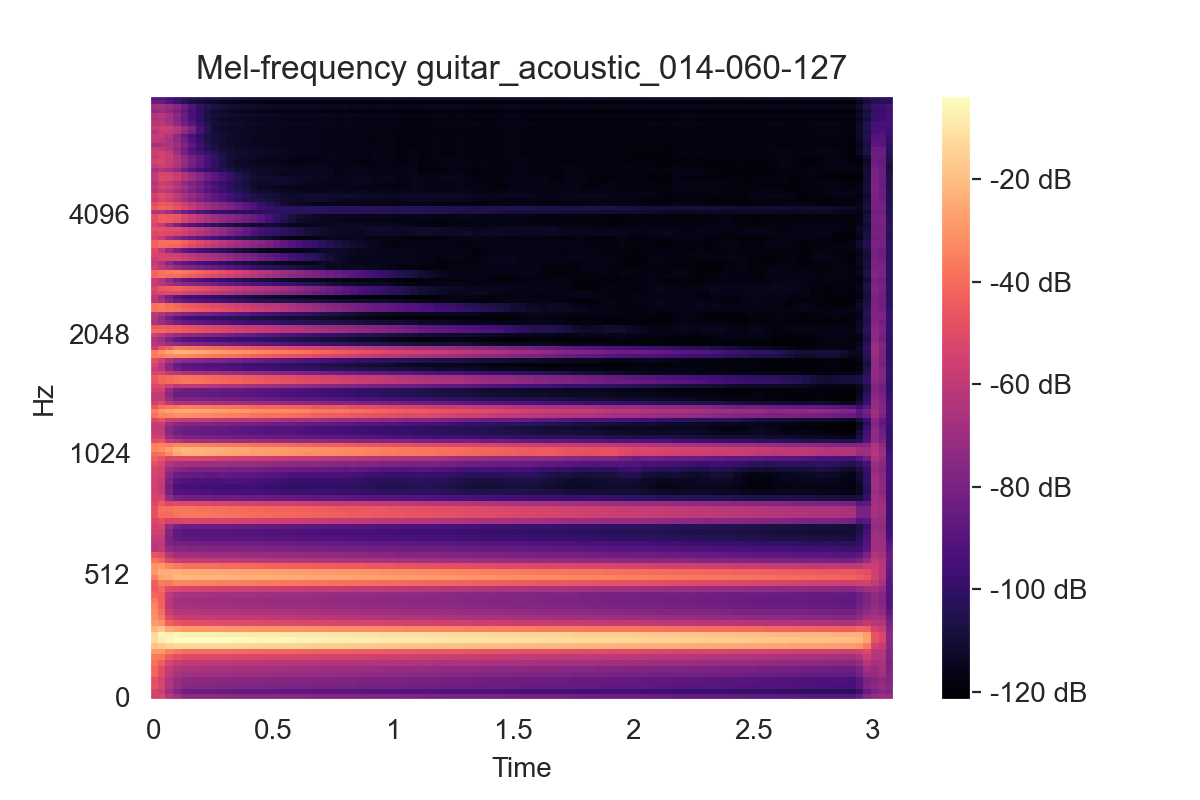
\includegraphics[width=0.55\textwidth]{images/results/mel_single_str/guitar_acoustic_014-060-127.png}}&
        \makebox{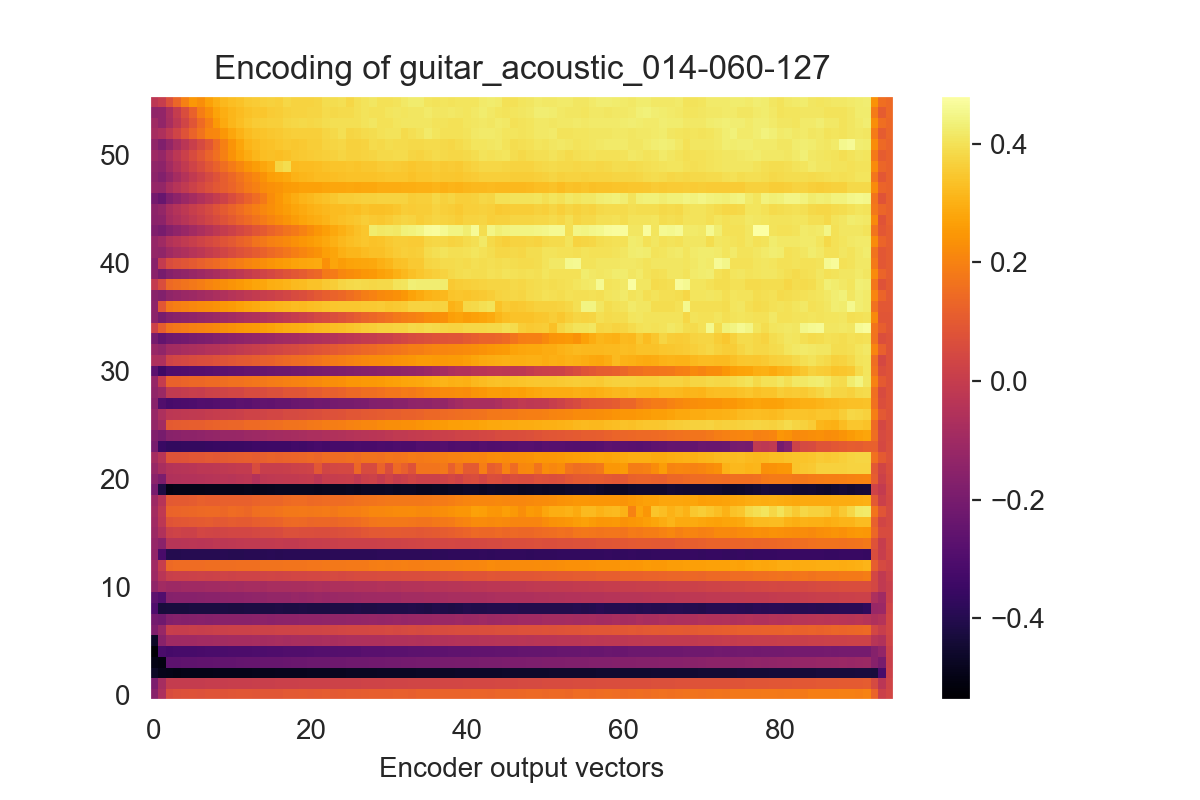
\includegraphics[width=0.55\textwidth]{images/results/mel_single_str/emb_guitar_acoustic_014-060-127.png}}\\
        (a) & (b)
    \end{tabular}}
    \caption{reconstruction of guitar acoustic ~(a), embedding of guitar acoustic ~(b)\\single stride model.}
    \label{fig:res_mel_single_str_2D_output_emb}
\end{figure}

In figure \ref{fig:res_mel_single_str_2D_output_emb}a the output of the single strided network can be seen. Comparing to the input spectrogram, its reconstruction is the best out of those three networks, as it contains the most details. Despite of this, it can be seen, that the broad band spectra at the beginning and end, are not as intense as with the input. Further on it can be seen, that changes over time in the frequencies between the lower harmonics, are not present in the output. The embeddings in figures \ref{fig:res_mel_single_str_2D_output_emb}b and \ref{fig:res_mel_double_str_2D_output_emb}b show that the features representing the lower harmonics, are recognizable as negative values. The latter already shows a lack of features in the higher harmonics. This is caused, because the input log-mel spectrograms have a shorter distance between the higher harmonics then in the lower ones. Regarding the output of the double-stride network it can therefore be said, that the higher harmonics can be less distinguished from each other then with the single-stride network (see area between >2048 Hz).


\begin{figure}[htb!]
    \centering
    \captionsetup{justification=centering}
    \makebox[\textwidth][c]{\begin{tabular}{@{}cc@{}}
        \makebox{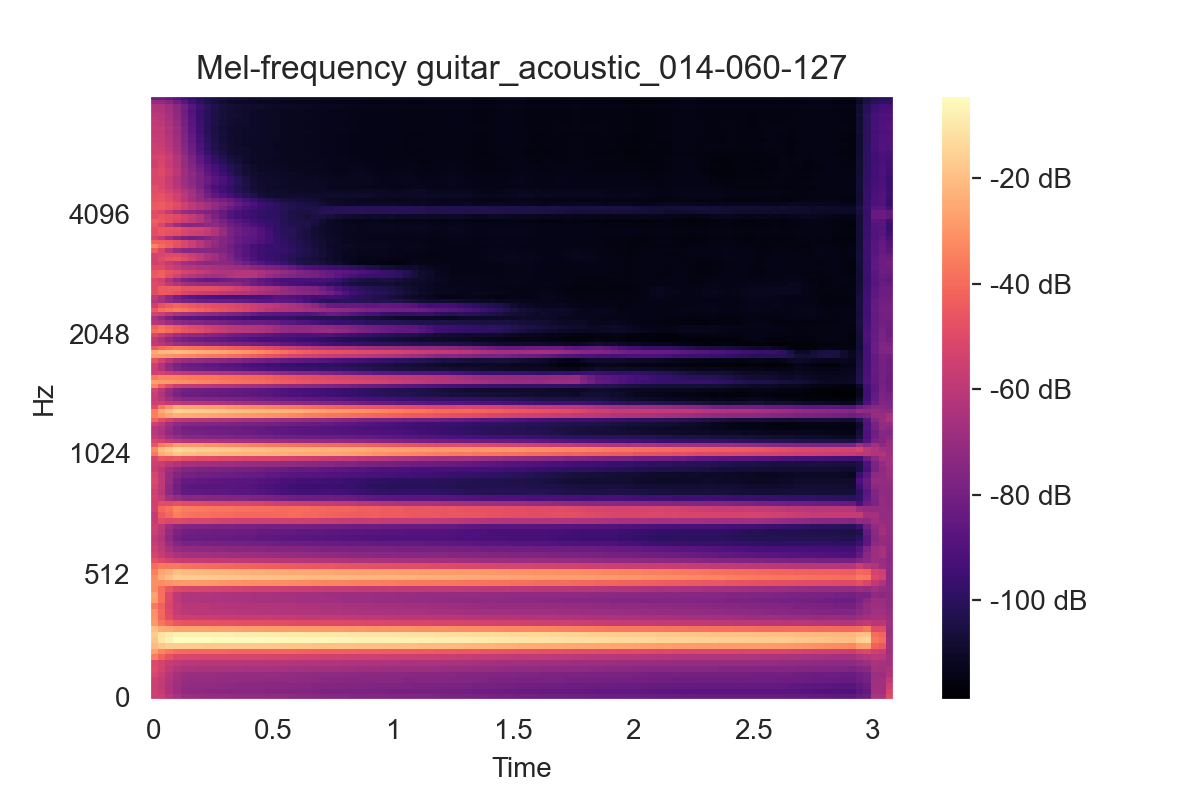
\includegraphics[width=0.55\textwidth]{images/results/mel_double_str/guitar_acoustic_014-060-127.png}}&
        \makebox{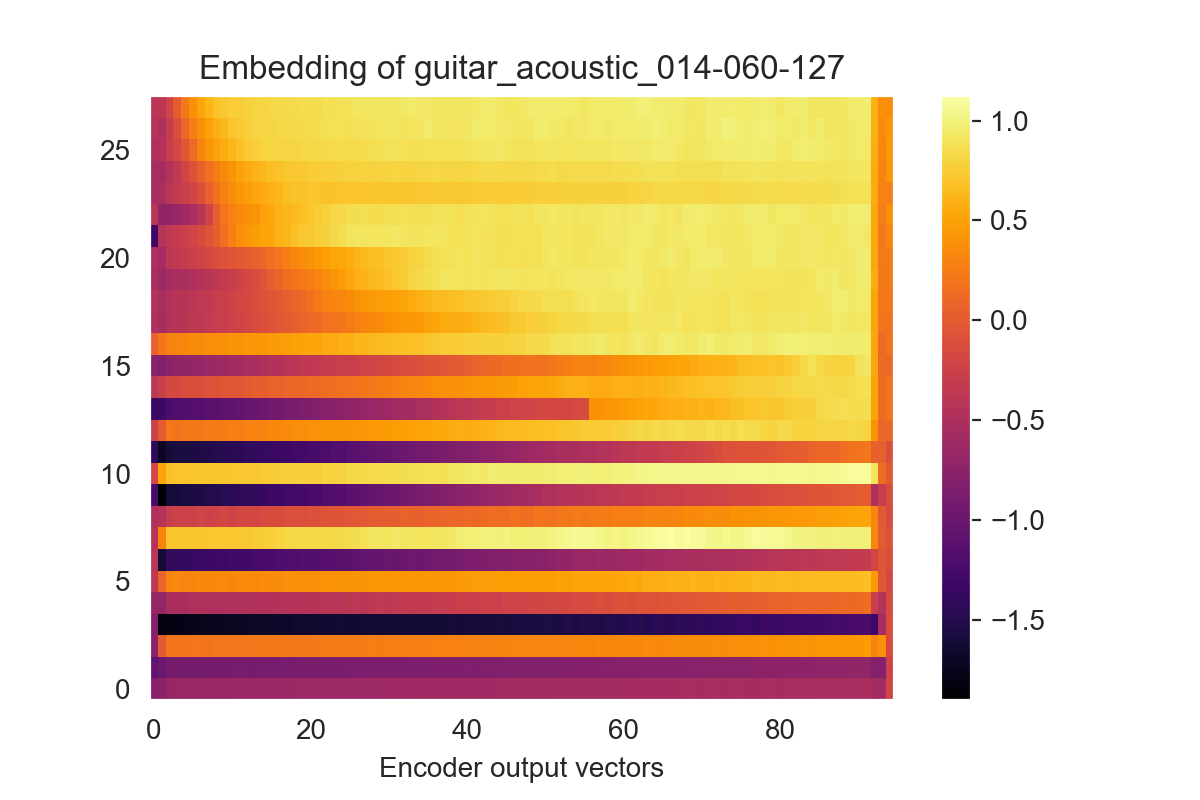
\includegraphics[width=0.55\textwidth]{images/results/mel_double_str/emb_guitar_acoustic_014-060-127.png}}\\
        (a) & (b)
    \end{tabular}}
    \caption{reconstruction of guitar acoustic ~(a), embedding of guitar acoustic ~(b)\\double stride model.}
    \label{fig:res_mel_double_str_2D_output_emb}
\end{figure}

Comparing the result of the double-strided networks with the one of the triple strided network, significant differences can be discovered. Especially when looking onto the embedding, it can be discovered, that due to the small amount of values on the y-axis the features are less distinguishable. Thus it is also more difficult to describe them. Nevertheless it can be said for this input spectrogram, that the colored areas still represent the most significant features that describe the input. Interestingly when looking onto the output spectrogram in \ref{fig:res_mel_triple_str_2D_output_emb}a, depending the lower harmonics, no differences can be seen to the previous output spectrograms. The part around 4096 Hz also shows some distinct spots that contain more energy, which are not present in the input spectrogram (artefacts).

\begin{figure}[htb!]
    \centering
    \captionsetup{justification=centering}
    \makebox[\textwidth][c]{\begin{tabular}{@{}cc@{}}
        \makebox{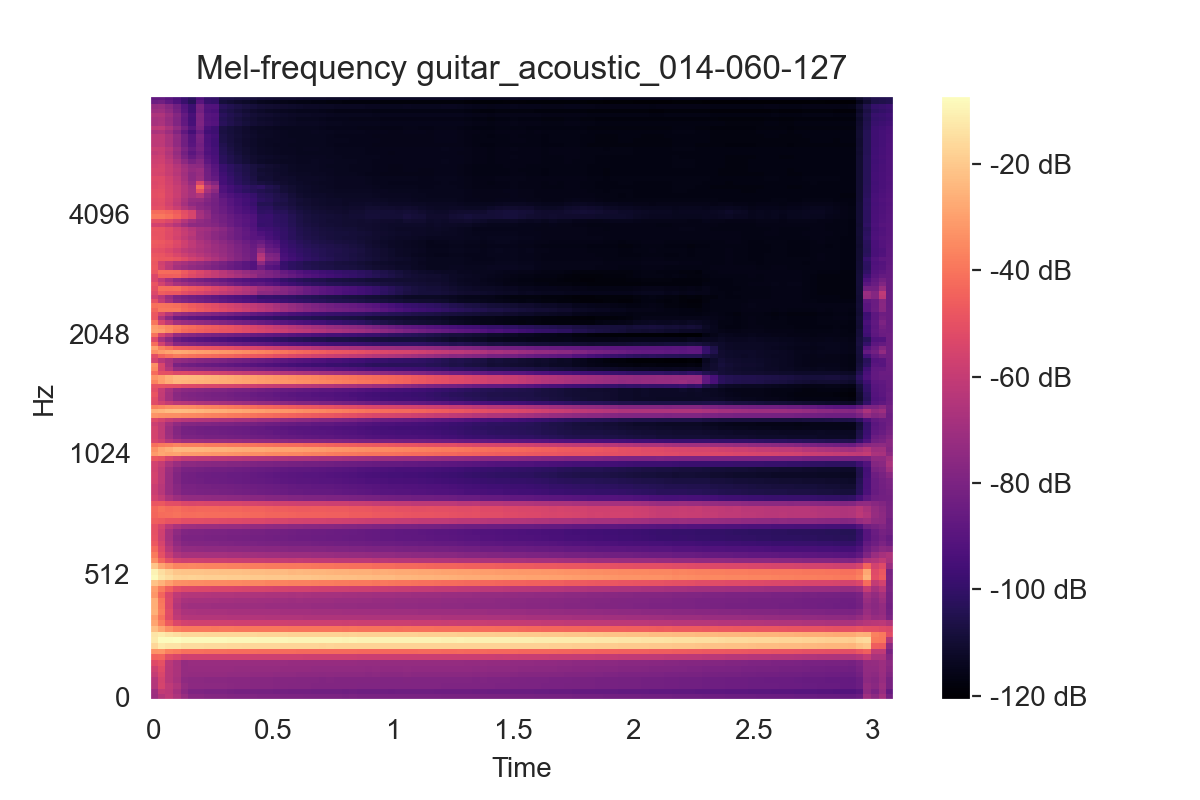
\includegraphics[width=0.55\textwidth]{images/results/mel_triple_str/guitar_acoustic_014-060-127.png}}&
        \makebox{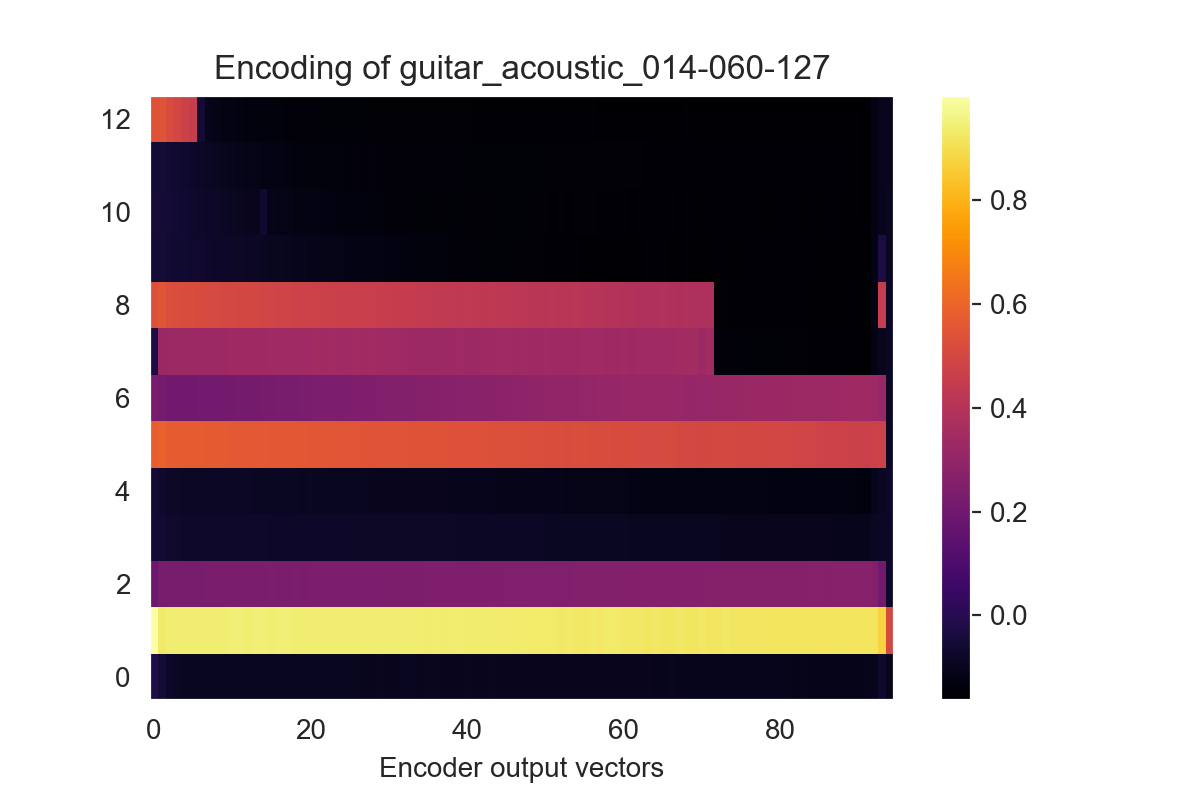
\includegraphics[width=0.55\textwidth]{images/results/mel_triple_str/emb_guitar_acoustic_014-060-127.png}}\\
        (a) & (b)
    \end{tabular}}
    \caption{reconstruction of guitar acoustic ~(a), Embedding of guitar acoustic ~(b)\\triple stride model.}
    \label{fig:res_mel_triple_str_2D_output_emb}
\end{figure}

\subsection{Experiments with interpolation in embedding}
The final experiments in this work also deal with the introduction of the interpolation step to synthesize novel sounds. With the experiments of reconstructing single audios, it could be seen that despite of the small compressed embeddings, the input spectrograms could be reconstructed adequately. Having those smaller embeddings, less values are available to reconstruct spectrograms which in conclusion means that altering those brings also significant changes. This fact makes these experiments even more interesting, as here again, the embeddings of two input samples, get interpolated, to generate a novel sounds. As an example, the same guitar and brass samples, that were used in the previous experiments, are utilized to synthesize audio. The following graphics \ref{fig:res_mel_original_guit_brass} show the input log-mel spectrograms of the two source signals. To mention at this point again, the higher harmonics are closer in the scale, while the lower harmonics have a greater distance. Especially when looking at the brass sample this can be noticed as the energy does not fade.

\begin{figure}[htb!]
    \centering
    \captionsetup{justification=centering}
    \makebox[\textwidth][c]{\begin{tabular}{@{}cc@{}}
        \makebox{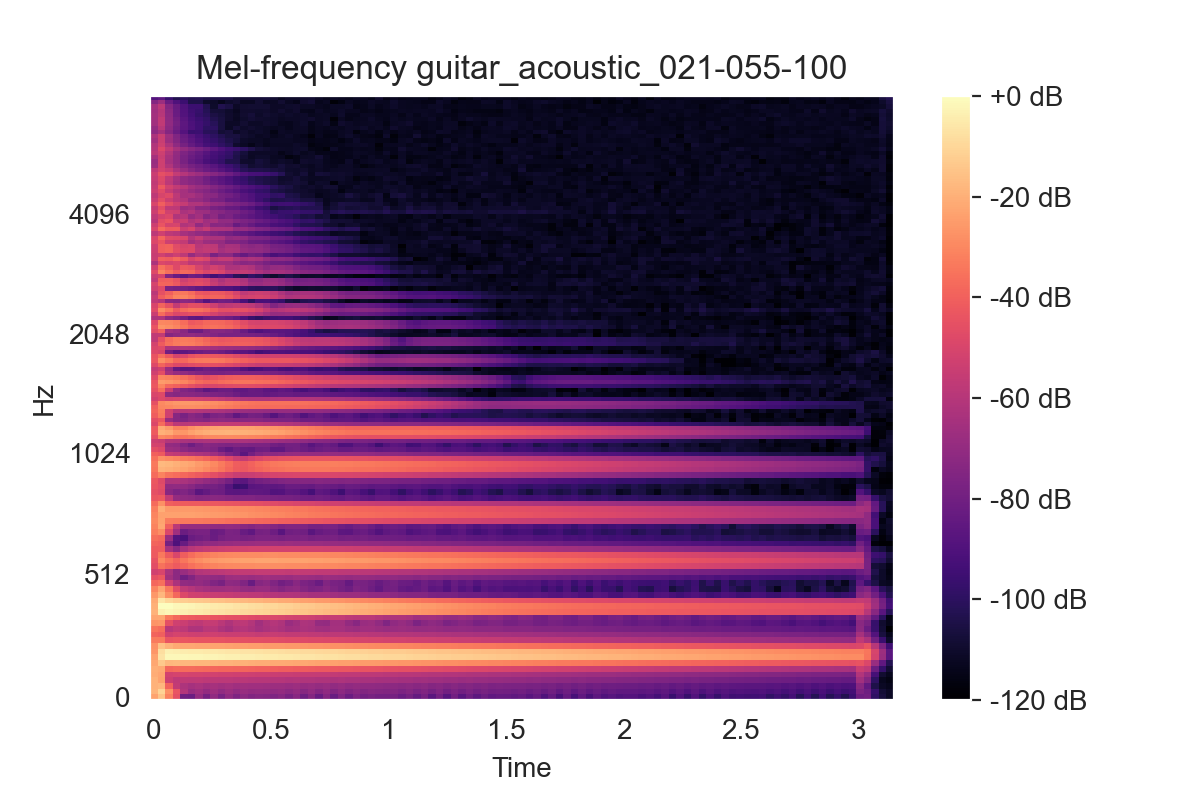
\includegraphics[width=0.55\textwidth]{images/results/mel_guitar_acoustic_021-055-100.png}}&
        \makebox{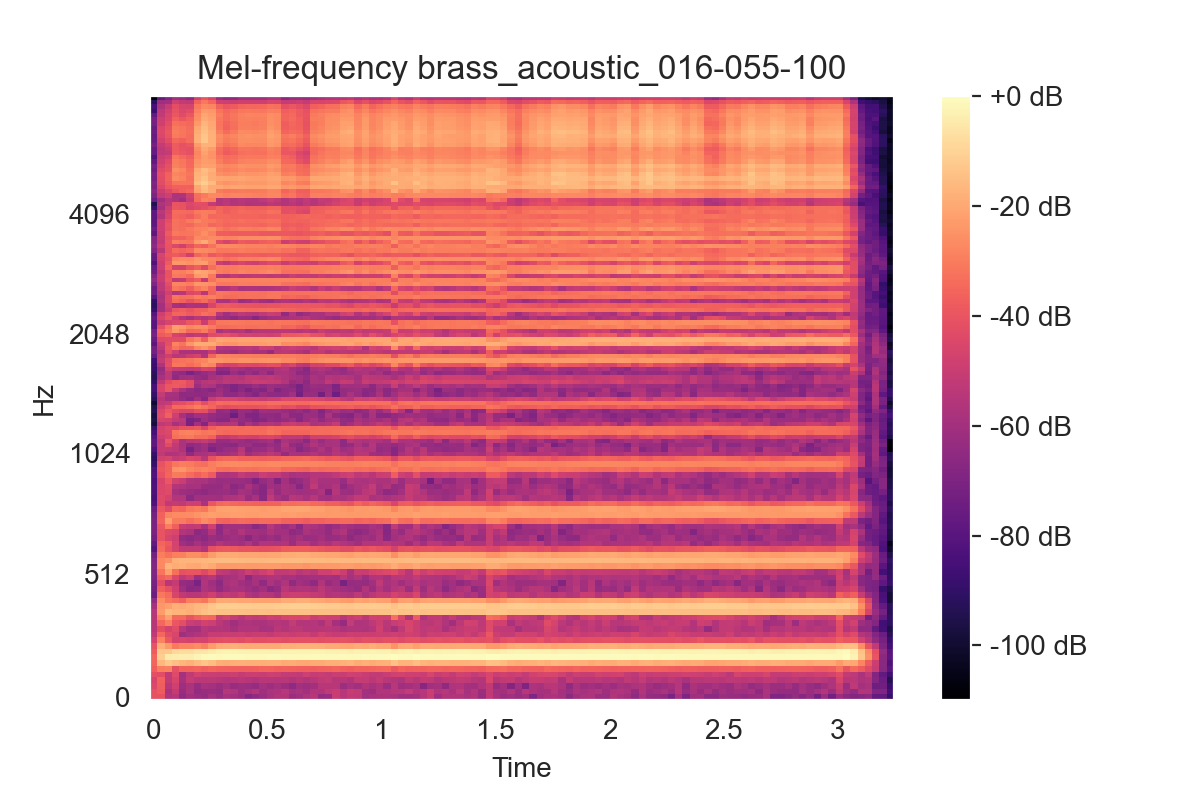
\includegraphics[width=0.55\textwidth]{images/results/mel_brass_acoustic_016-055-100.png}}\\
        (a) & (b)
    \end{tabular}}
    \caption{original guitar acoustic ~(a), original brass acoustic
    ~(b)}
    \label{fig:res_mel_original_guit_brass}
\end{figure}

Knowing the source log-mel spectrograms, the following graphics show the embeddings of those spectrograms, the interpolated embedding as well as the resulting output spectrogram using again the three differently strided networks (single-, double- and triple-stride). By comparing all the output spectrograms to the two input spectrograms, it again can be said, that the output of the single stride network in figure \ref{fig:res_mel_single_str_2D_inter_output}b is the most precise and contains the most of both instruments. The upper harmonics of the brass sample can still be recognized in the output spectrogram despite the "fading" influence of the guitar sample. Fine changes in the harmonics over time of the trumpet, like at second 1.5, cannot be recognized anymore. Furthermore the guitar sample can also be recognized in the output spectrogram. With a look onto the embeddings those again show the high energy areas with low or negative values. The original low energy areas in turn have positive values. Furthermore due to the little distance between the higher frequency ranges in the input log-mel spectrograms, the embeddings in this area just depict the high-energy areas. This leads the output spectrogram to not have a high precision in the higher harmonics. Nevertheless through interpolation the resulting embedding contains features of both instruments as well as the resulting spectrogram. 

\begin{figure}[htb!]
    \centering
    \makebox[\textwidth][c]{\begin{tabular}{@{}cc@{}}
        \makebox{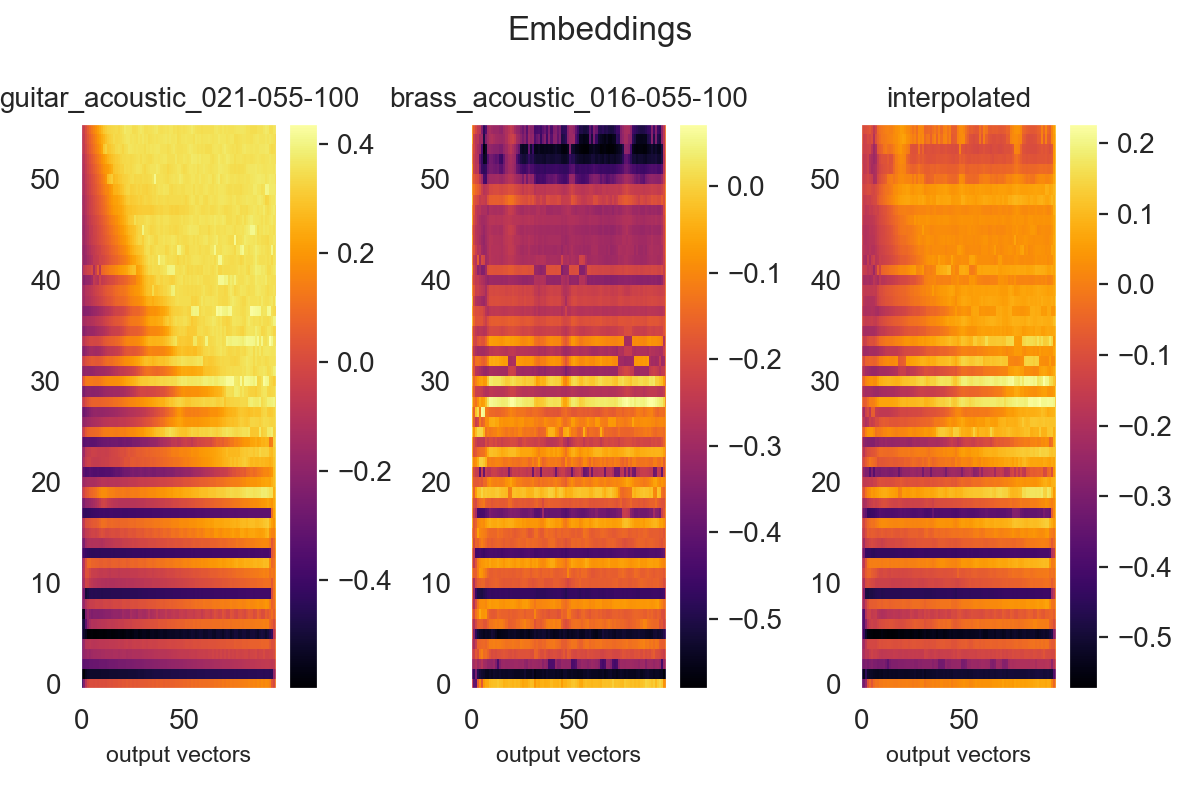
\includegraphics[width=0.55\textwidth]{images/results/mel_single_str/inter_guitar_acoustic_021-055-100&brass_acoustic_016-055-100_original_0.5.png}}&
        \makebox{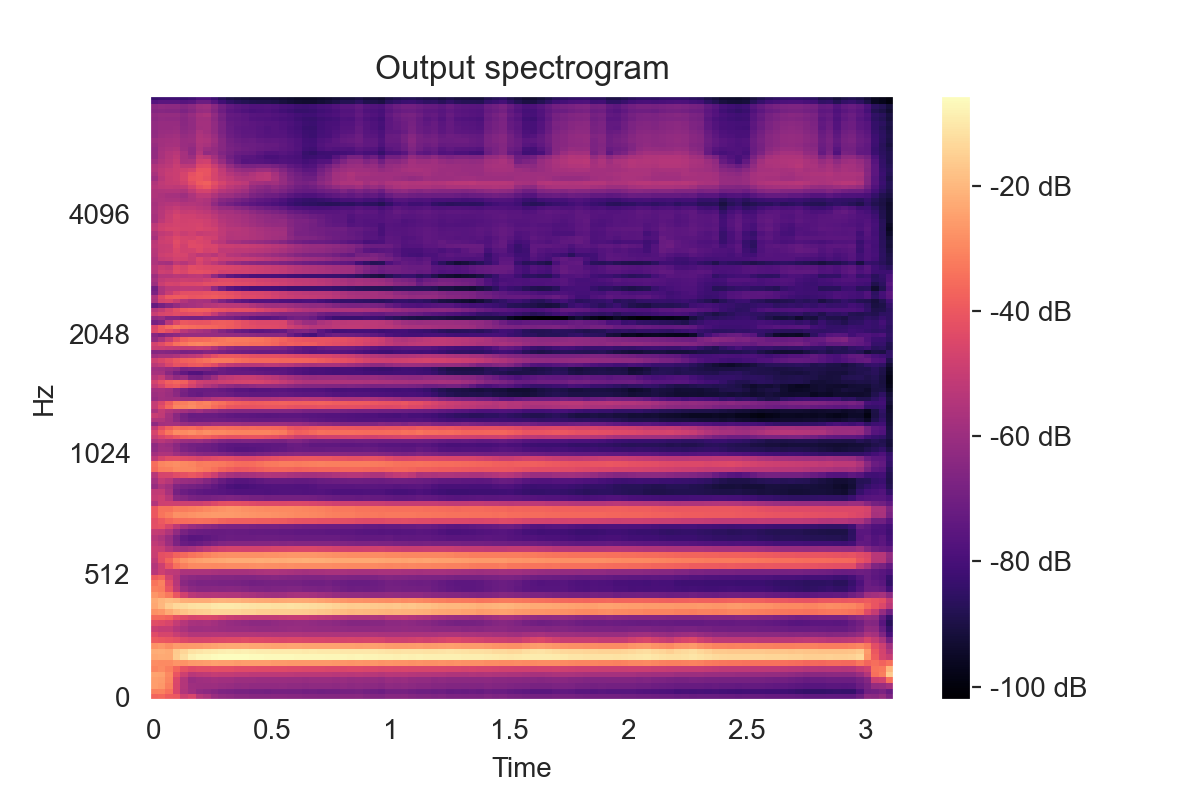
\includegraphics[width=0.55\textwidth]{images/results/mel_single_str/guitar_acoustic_021-055-100&brass_acoustic_016-055-100_output_0.5.png}}\\
        (a) & (b)
    \end{tabular}}
    \caption{embedding interpolation ~(a), output signal ~(b).}
    \label{fig:res_mel_single_str_2D_inter_output}
\end{figure}

The next figure \ref{fig:res_mel_double_str_2D_inter_output}, shows the output, of the double-stride network where already significant differences to the output of the single-strided network can be seen. First of all regarding the embeddings, the features representing the higher harmonics of both instruments (range >=15) are less intense while the features of the lower harmonics, are still distinguishable. Having the interpolated embedding the features of both embeddings can be still recognized, despite the less precision in the y-axis above 15. As a result the output spectrogram, the higher harmonics of both instruments are rather "washed out" and appear blurry in the spectrogram. 

\begin{figure}[htb!]
    \centering
    \makebox[\textwidth][c]{\begin{tabular}{@{}cc@{}}
        \makebox{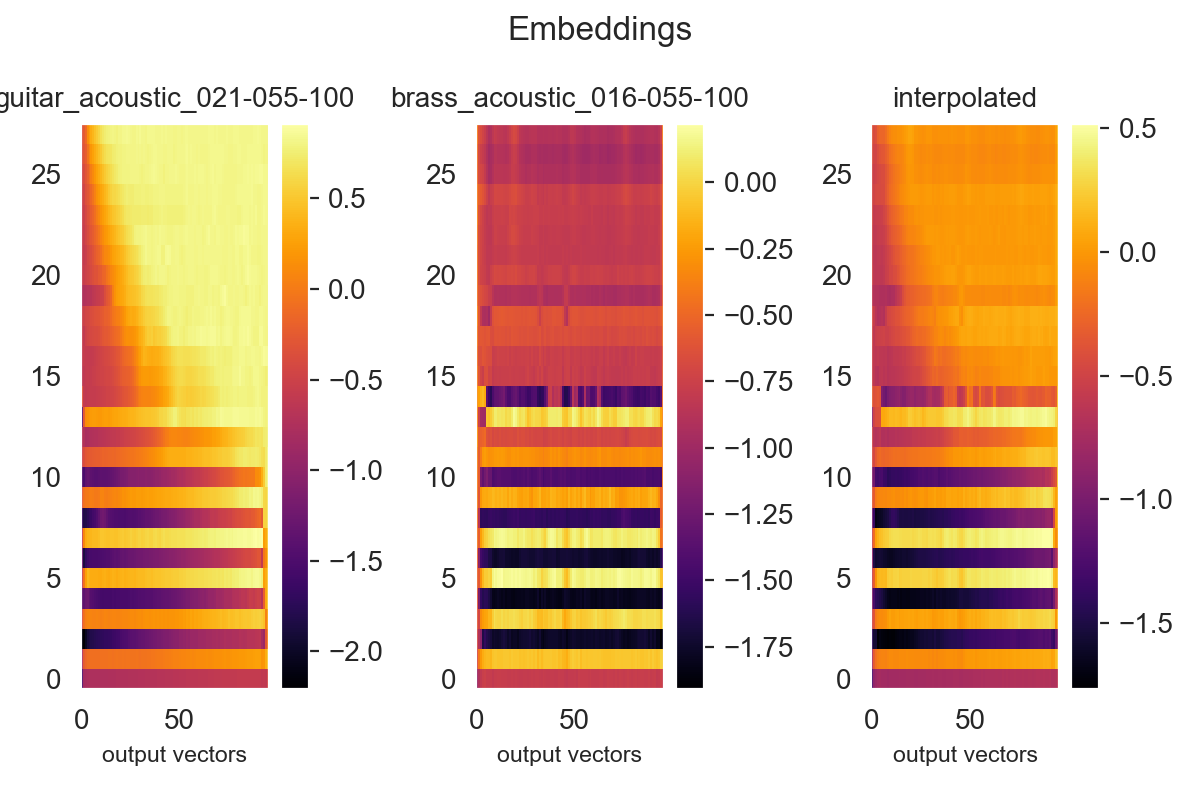
\includegraphics[width=0.55\textwidth]{images/results/mel_double_str/inter_guitar_acoustic_021-055-100&brass_acoustic_016-055-100_original_0.5.png}}&
        \makebox{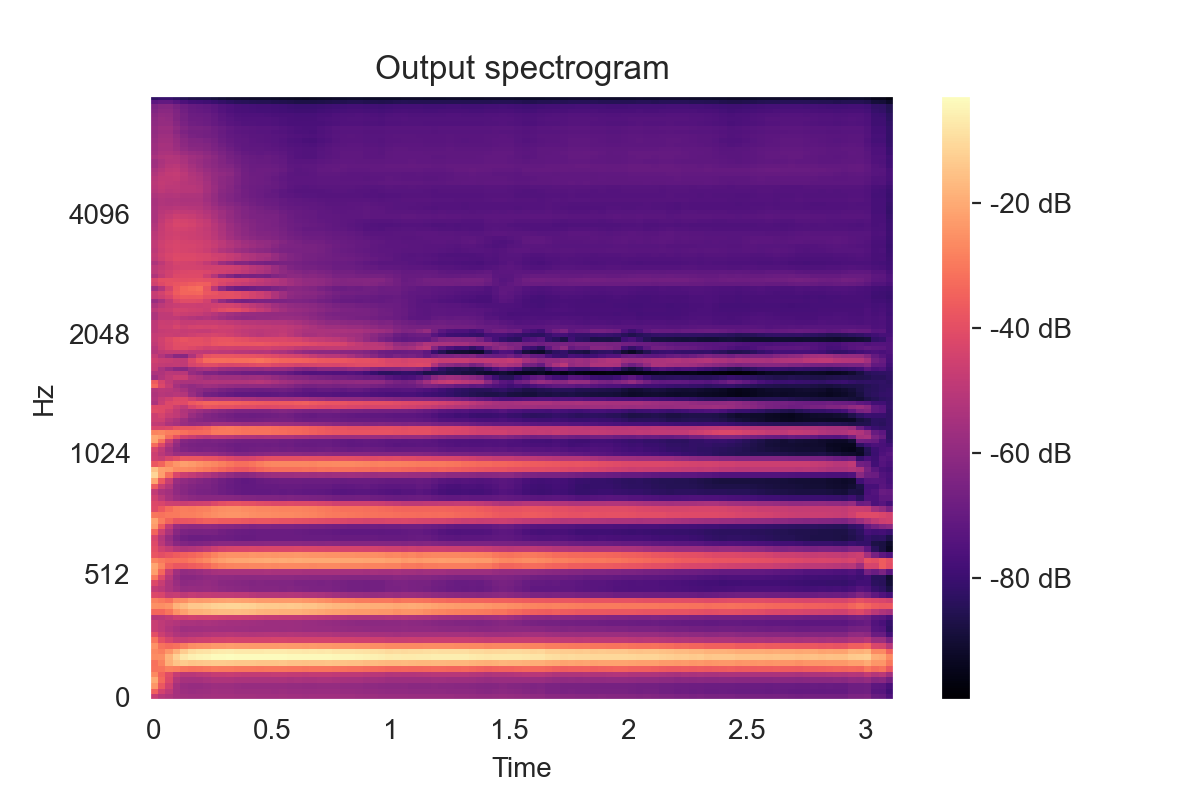
\includegraphics[width=0.55\textwidth]{images/results/mel_double_str/guitar_acoustic_021-055-100&brass_acoustic_016-055-100_output_0.5.png}}\\
        (a) & (b)
    \end{tabular}}
    \caption{embedding interpolation ~(a), output signal ~(b).}
    \label{fig:res_mel_double_str_2D_inter_output}
\end{figure}

Coming to the output of the triple-stride network, here it can be seen that the features contained in the embeddings have no common structure with the input spectrograms. The values therefore cannot be described sufficiently. Also those appear different to the one depicted in figure \ref{fig:res_mel_triple_str_2D_output_emb}b. When looking at the output spectrogram generated of the interpolated embedding, it can be seen that in the area around 1024 to 2048 significant energy changes regarding certain frequencies are present which cannot be recognized in the input. Similar to the output of the previous network in figure \ref{fig:res_mel_double_str_2D_inter_output}b fine structures of the input are also not present anymore. 

\begin{figure}[htb!]
    \centering
    \makebox[\textwidth][c]{\begin{tabular}{@{}cc@{}}
        \makebox{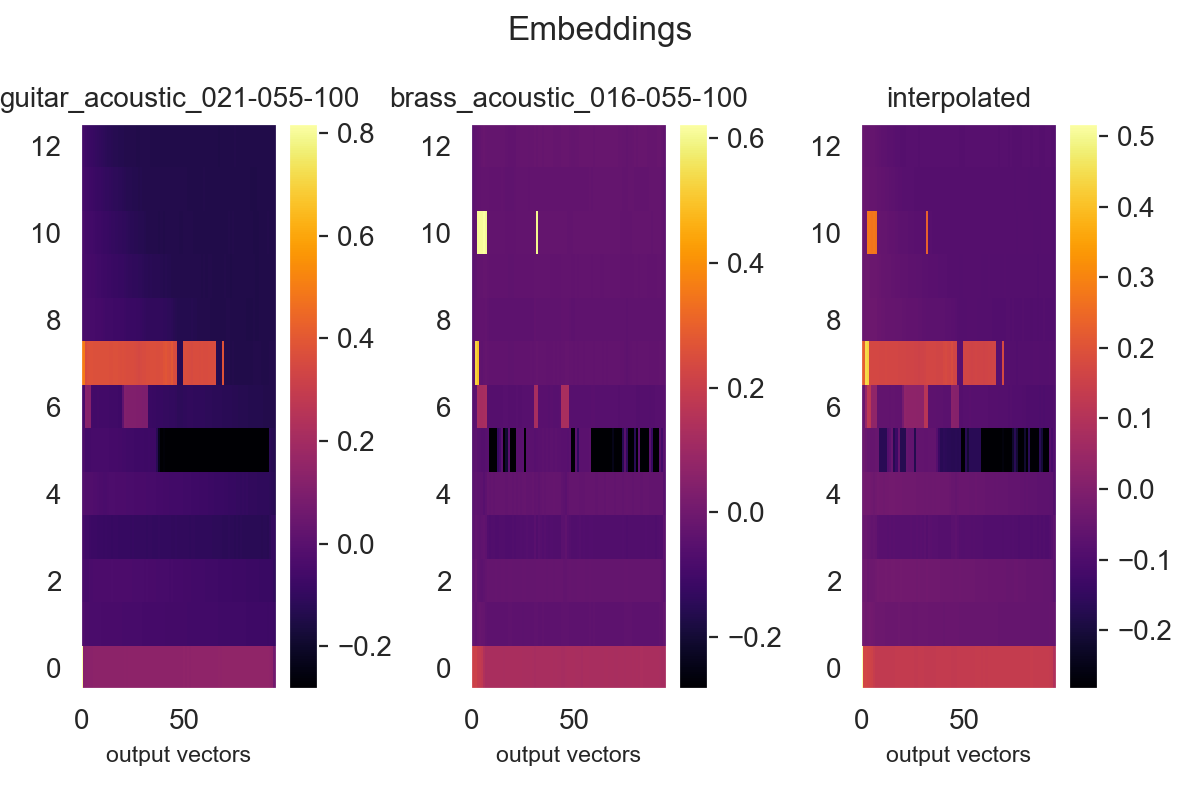
\includegraphics[width=0.55\textwidth]{images/results/mel_triple_str/inter_guitar_acoustic_021-055-100&brass_acoustic_016-055-100_original_0.5.png}}&
        \makebox{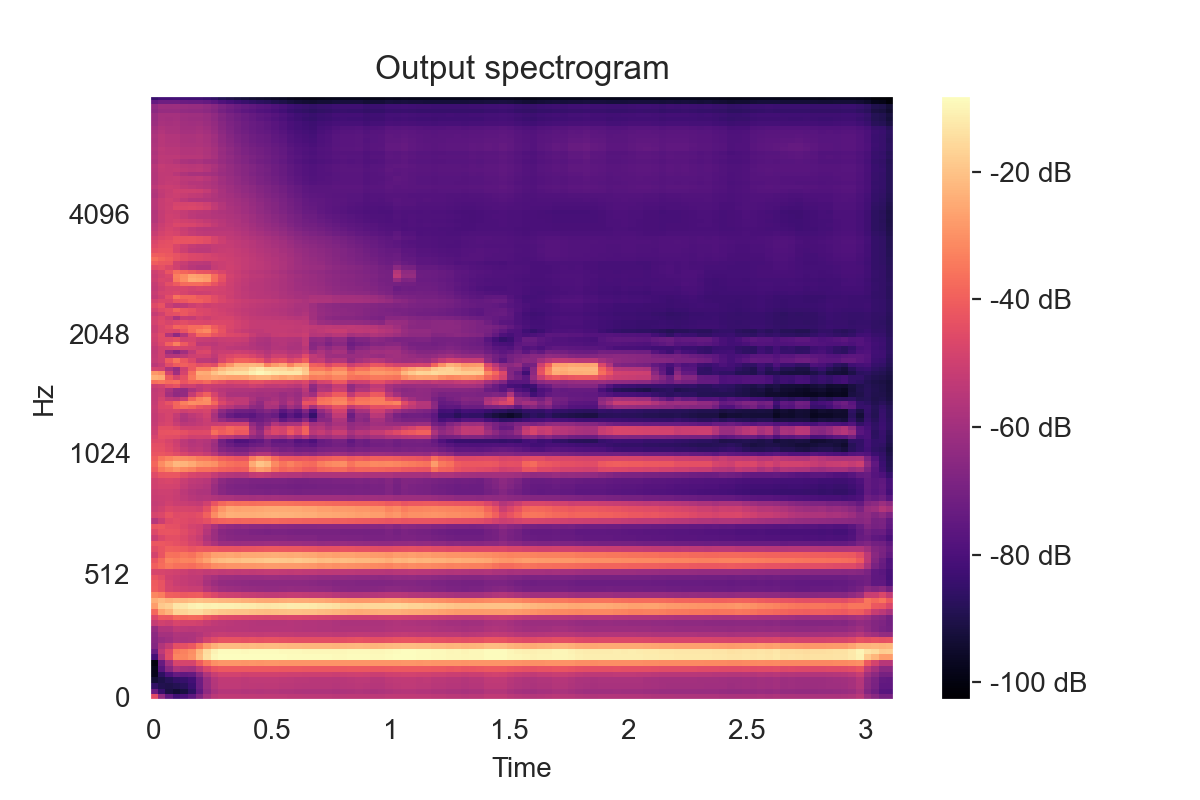
\includegraphics[width=0.55\textwidth]{images/results/mel_triple_str/guitar_acoustic_021-055-100&brass_acoustic_016-055-100_output_0.5.png}}\\
        (a) & (b)
    \end{tabular}}
    \caption{embedding interpolation ~(a), output signal ~(b).}
    \label{fig:res_mel_triple_str_2D_inter_output}
\end{figure}
\chapter{Discussion/Evaluation}
\label{cha:Discussion}

\section{Interpretation of results / observations}

\subsection{Quality of audio}

\subsection{Differences between instruments}

\subsection{Impact of model configurations}

\subsection{Impact of pre processing}

\subsection{Impact of post-processing}

\section{Comparison to other approaches}

\section{Limitations/difficulties}

\section{Outlook}

The listenable sounds / output sounds of the networks get discussed at this point.

%Snippet of 1D conv net interpolated output
By listening to the final obtained sample, it can be heard, that it already contains features of both instruments despite the guitar is not as present as expected (guitar stroke not audible). Furthermore the sound contains distortion which is not desirable.
\chapter{Conclusion}
\label{cha:Conclusion}
%\chapter{Future Work}
\label{cha:FutureWork}



%%%-----------------------------------------------------------------------------
\appendix                                                             % Appendix 
%%%-----------------------------------------------------------------------------

\chapter{Additional Graphics}
\label{app:addional_graphics}


\begin{figure}[htb!]
    \centering
    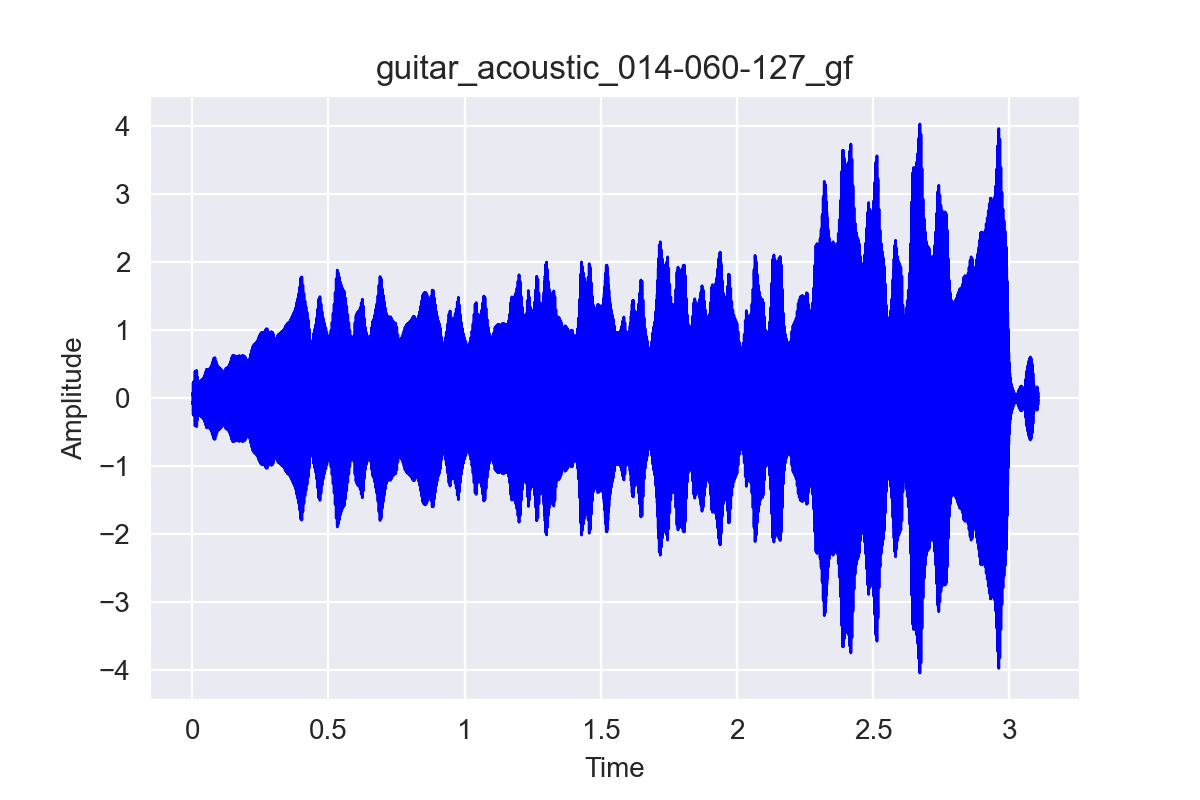
\includegraphics[width=0.55\textwidth]{images/appendix/1D/guitar_acoustic_014-060-127_gf.png}
    \caption{guitar acoustic output with griffin lim (1D conv).}
    \label{fig:res_2D_mel_guit}
\end{figure}


\begin{figure}[htb!]
    \centering
    \captionsetup{justification=centering}
    \makebox[\textwidth][c]{\begin{tabular}{@{}cc@{}}
        \makebox{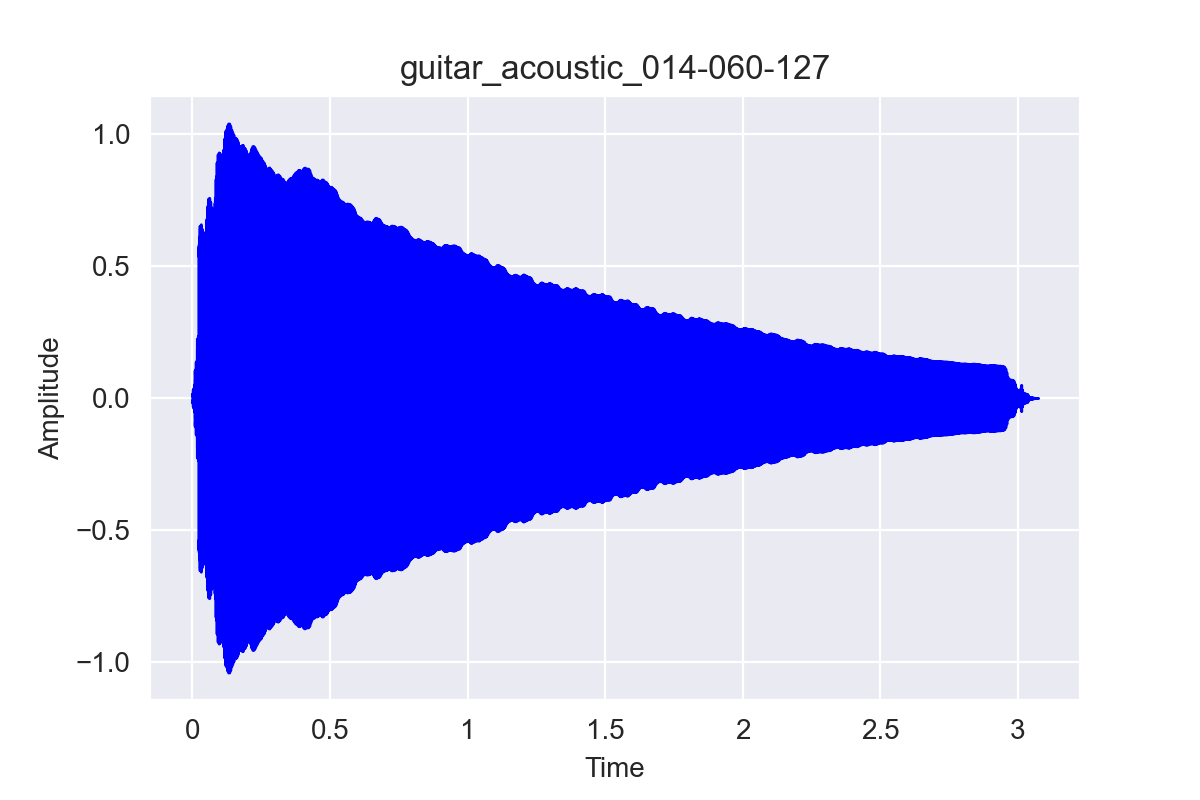
\includegraphics[width=0.55\textwidth]{images/appendix/single_stride/guitar_acoustic_014-060-127.png}}&
        \makebox{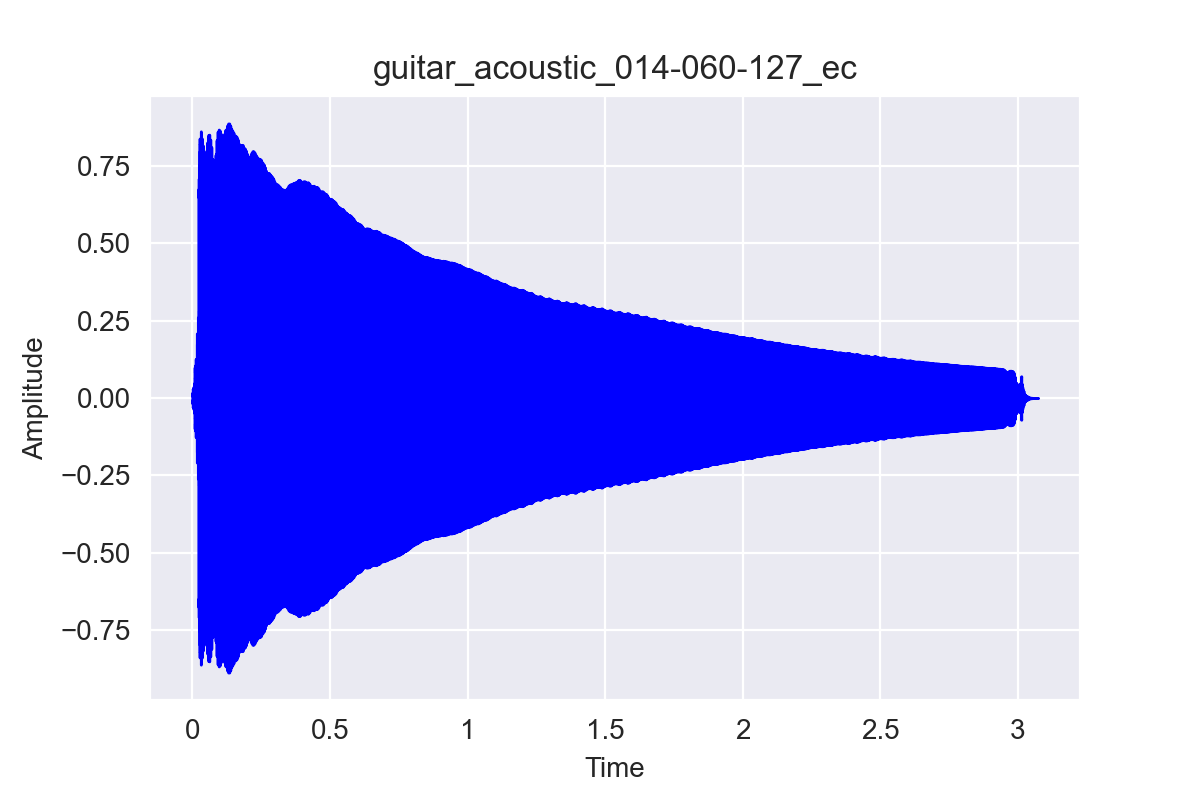
\includegraphics[width=0.55\textwidth]{images/appendix/single_stride/guitar_acoustic_014-060-127_ec.png}}\\
        (a) & (b)
    \end{tabular}}
    \caption{2D convolutional single-stride network - guitar acoustic output without post processing ~(a), output with post processing ~(b).}
    \label{fig:apx_single_phase}
\end{figure}

\begin{figure}[htb!]
    \centering
    \captionsetup{justification=centering}
    \makebox[\textwidth][c]{\begin{tabular}{@{}cc@{}}
        \makebox{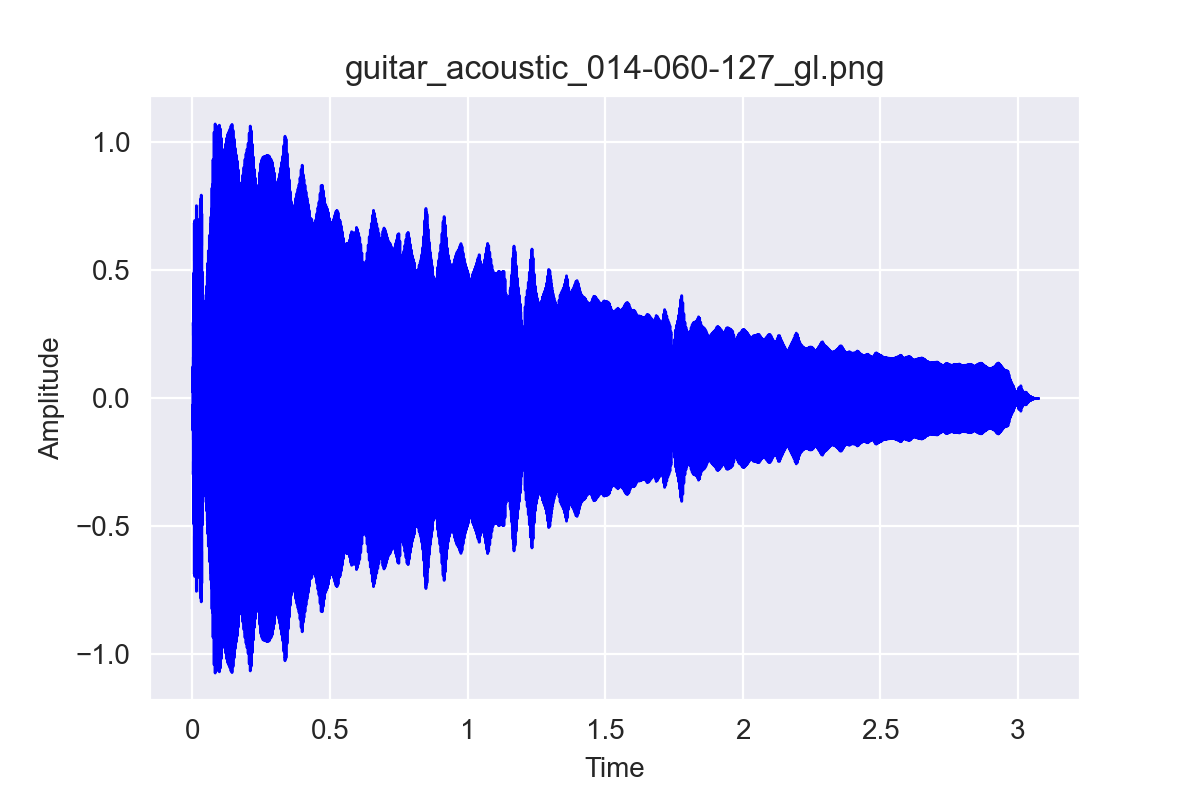
\includegraphics[width=0.55\textwidth]{images/appendix/single_stride/guitar_acoustic_014-060-127_gl.png}}&
        \makebox{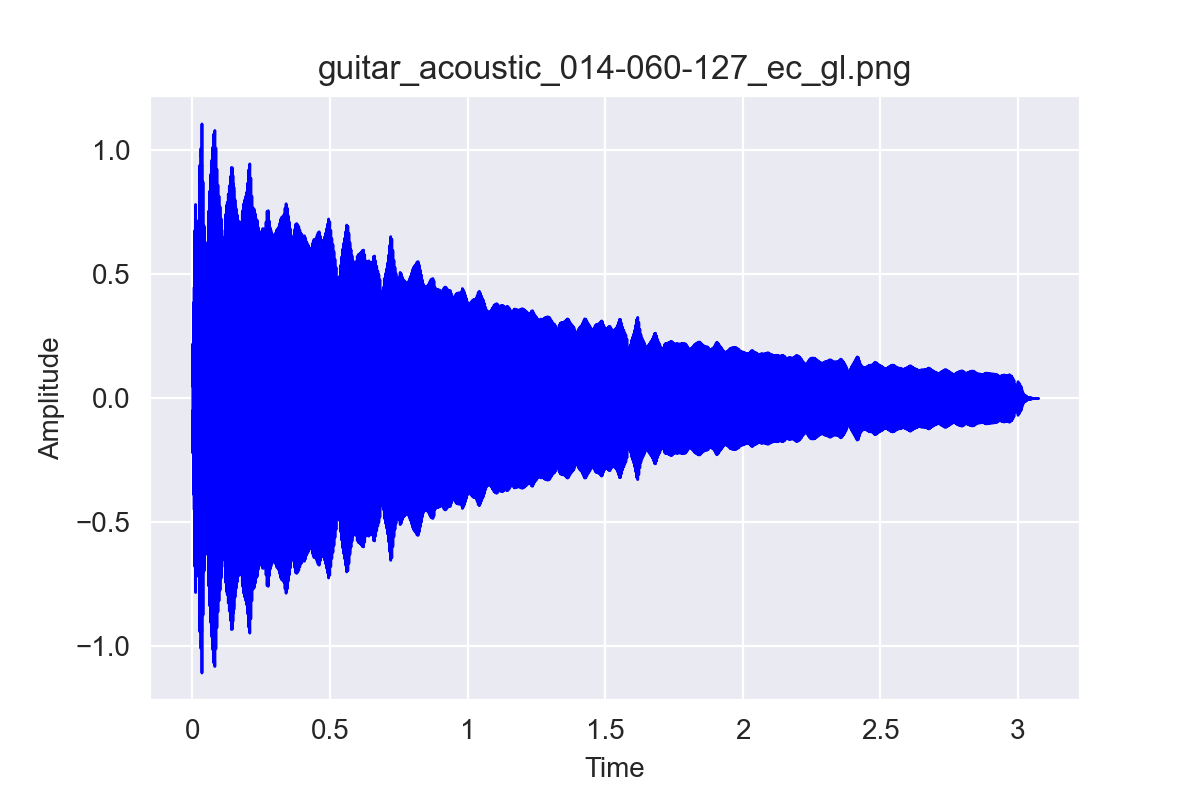
\includegraphics[width=0.55\textwidth]{images/appendix/single_stride/guitar_acoustic_014-060-127_ec_gl.png}}\\
        (a) & (b)
    \end{tabular}}
    \caption{2D convolutional single-stride network - guitar acoustic output without post processing and Griffin Lim ~(a), output with post processing and Griffin Lim ~(b).}
    \label{fig:apx_single_gf}
\end{figure}

\begin{figure}[htb!]
    \centering
    \captionsetup{justification=centering}
    \makebox[\textwidth][c]{\begin{tabular}{@{}cc@{}}
        \makebox{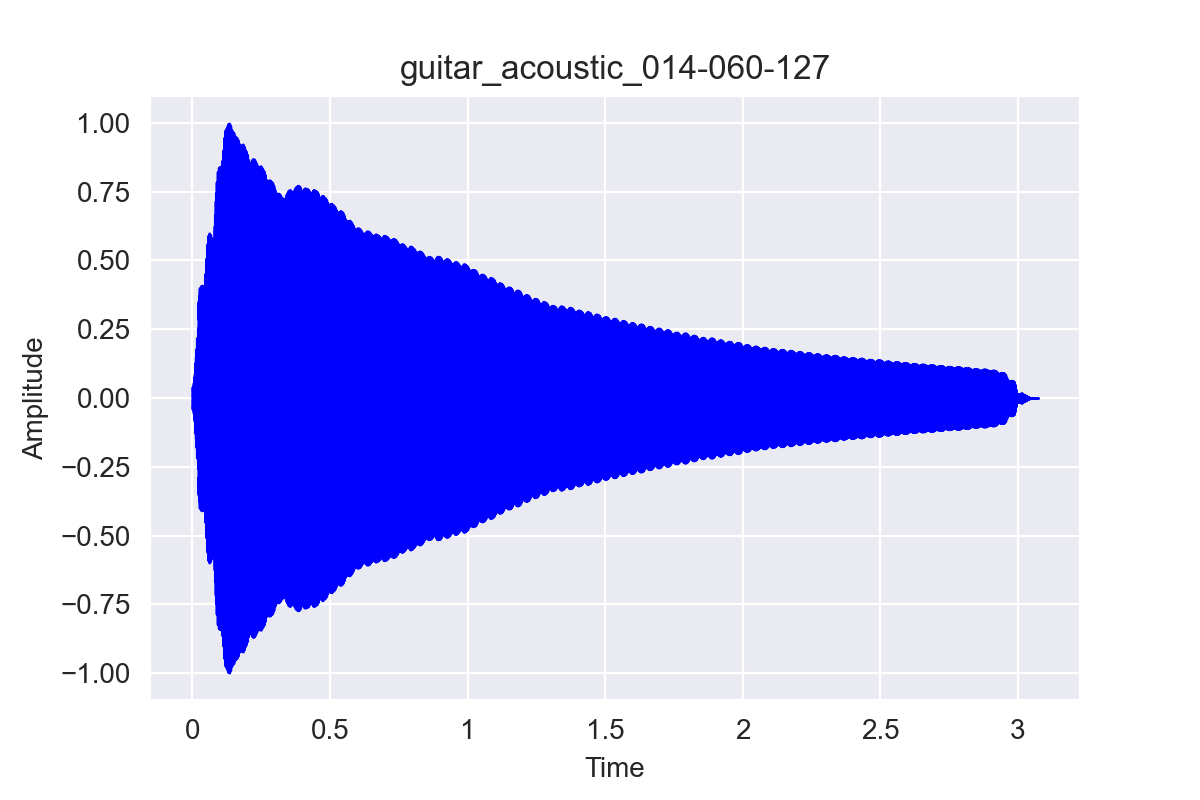
\includegraphics[width=0.55\textwidth]{images/appendix/double_stride/guitar_acoustic_014-060-127.png}}&
        \makebox{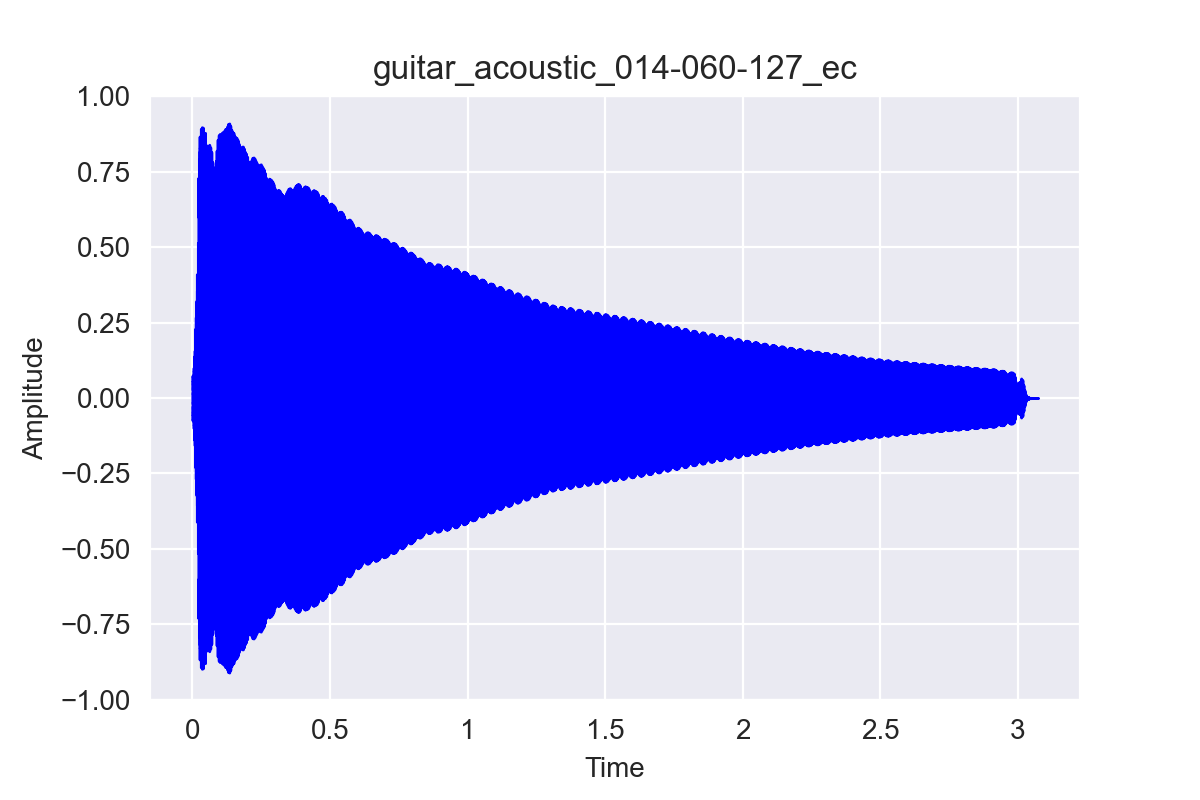
\includegraphics[width=0.55\textwidth]{images/appendix/double_stride/guitar_acoustic_014-060-127_ec.png}}\\
        (a) & (b)
    \end{tabular}}
    \caption{2D convolutional double-stride network - guitar acoustic output without post processing ~(a), output with post processing ~(b).}
    \label{fig:apx_double_phase}
\end{figure}

\begin{figure}[htb!]
    \centering
    \captionsetup{justification=centering}
    \makebox[\textwidth][c]{\begin{tabular}{@{}cc@{}}
        \makebox{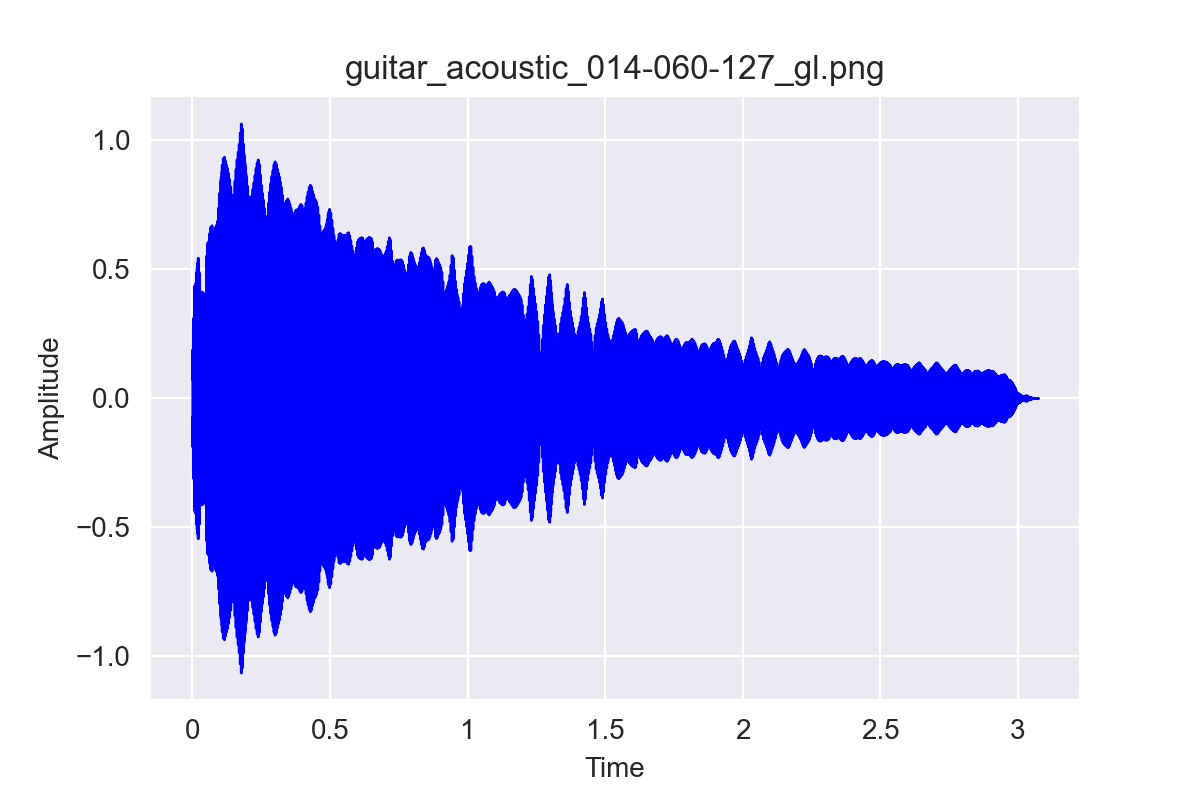
\includegraphics[width=0.55\textwidth]{images/appendix/double_stride/guitar_acoustic_014-060-127_gl.png}}&
        \makebox{\includegraphics[width=0.55\textwidth]{images/appendix/double_stride/guitar_acoustic_014-060-127_ec_gl.png}}\\
        (a) & (b)
    \end{tabular}}
    \caption{2D convolutional double-stride network - guitar acoustic output without post processing and Griffin Lim ~(a), output with post processing and Griffin Lim ~(b).}
    \label{fig:apx_double_gf}
\end{figure}

\begin{figure}[htb!]
    \centering
    \captionsetup{justification=centering}
    \makebox[\textwidth][c]{\begin{tabular}{@{}cc@{}}
        \makebox{\includegraphics[width=0.55\textwidth]{images/appendix/triple_stride/guitar_acoustic_014-060-127.png}}&
        \makebox{\includegraphics[width=0.55\textwidth]{images/appendix/triple_stride/guitar_acoustic_014-060-127_ec.png}}\\
        (a) & (b)
    \end{tabular}}
    \caption{2D convolutional triple-stride network - guitar acoustic output without post processing ~(a), output with post processing ~(b).}
    \label{fig:apx_triple_phase}
\end{figure}

\begin{figure}[htb!]
    \centering
    \captionsetup{justification=centering}
    \makebox[\textwidth][c]{\begin{tabular}{@{}cc@{}}
        \makebox{\includegraphics[width=0.55\textwidth]{images/appendix/triple_stride/guitar_acoustic_014-060-127_gl.png}}&
        \makebox{\includegraphics[width=0.55\textwidth]{images/appendix/triple_stride/guitar_acoustic_014-060-127_ec_gl.png}}\\
        (a) & (b)
    \end{tabular}}
    \caption{2D convolutional triple-stride network - guitar acoustic output without post processing and Griffin Lim ~(a), output with post processing and Griffin Lim ~(b).}
    \label{fig:apx_triple_gf}
\end{figure}


\begin{figure}[htb!]
    \centering
    \captionsetup{justification=centering}
    \makebox[\textwidth][c]{\begin{tabular}{@{}cc@{}}
        \makebox{\includegraphics[width=0.55\textwidth]{images/appendix/mel_single_stride/guitar_acoustic_014-060-127.png}}&
        \makebox{\includegraphics[width=0.55\textwidth]{images/appendix/mel_single_stride/guitar_acoustic_014-060-127_ec.png}}\\
        (a) & (b)
    \end{tabular}}
    \caption{2D convolutional single-stride network (log-mel) - guitar acoustic output without post processing ~(a), output with post processing ~(b).}
    \label{fig:apx_mel_single_phase}
\end{figure}

\begin{figure}[htb!]
    \centering
    \captionsetup{justification=centering}
    \makebox[\textwidth][c]{\begin{tabular}{@{}cc@{}}
        \makebox{\includegraphics[width=0.55\textwidth]{images/appendix/mel_single_stride/guitar_acoustic_014-060-127_gl.png}}&
        \makebox{\includegraphics[width=0.55\textwidth]{images/appendix/mel_single_stride/guitar_acoustic_014-060-127_ec_gl.png}}\\
        (a) & (b)
    \end{tabular}}
    \caption{2D convolutional single-stride network (log-mel) - guitar acoustic output without post processing and Griffin Lim ~(a), output with post processing and Griffin Lim ~(b).}
    \label{fig:apx_mel_single_gf}
\end{figure}

\begin{figure}[htb!]
    \centering
    \captionsetup{justification=centering}
    \makebox[\textwidth][c]{\begin{tabular}{@{}cc@{}}
        \makebox{\includegraphics[width=0.55\textwidth]{images/appendix/mel_double_stride/guitar_acoustic_014-060-127.png}}&
        \makebox{\includegraphics[width=0.55\textwidth]{images/appendix/mel_double_stride/guitar_acoustic_014-060-127_ec.png}}\\
        (a) & (b)
    \end{tabular}}
    \caption{2D convolutional double-stride network (log-mel) - guitar acoustic output without post processing ~(a), output with post processing ~(b).}
    \label{fig:apx_mel_double_phase}
\end{figure}

\begin{figure}[htb!]
    \centering
    \captionsetup{justification=centering}
    \makebox[\textwidth][c]{\begin{tabular}{@{}cc@{}}
        \makebox{\includegraphics[width=0.55\textwidth]{images/appendix/mel_double_stride/guitar_acoustic_014-060-127_gl.png}}&
        \makebox{\includegraphics[width=0.55\textwidth]{images/appendix/mel_double_stride/guitar_acoustic_014-060-127_ec_gl.png}}\\
        (a) & (b)
    \end{tabular}}
    \caption{2D convolutional double-stride network (log-mel) - guitar acoustic output without post processing and Griffin Lim ~(a), output with post processing and Griffin Lim ~(b).}
    \label{fig:apx_mel_double_gf}
\end{figure}

\begin{figure}[htb!]
    \centering
    \captionsetup{justification=centering}
    \makebox[\textwidth][c]{\begin{tabular}{@{}cc@{}}
        \makebox{\includegraphics[width=0.55\textwidth]{images/appendix/mel_triple_stride/guitar_acoustic_014-060-127.png}}&
        \makebox{\includegraphics[width=0.55\textwidth]{images/appendix/mel_triple_stride/guitar_acoustic_014-060-127_ec.png}}\\
        (a) & (b)
    \end{tabular}}
    \caption{2D convolutional triple-stride network (log-mel) - guitar acoustic output without post processing ~(a), output with post processing ~(b).}
    \label{fig:apx_mel_triple_phase}
\end{figure}

\begin{figure}[htb!]
    \centering
    \captionsetup{justification=centering}
    \makebox[\textwidth][c]{\begin{tabular}{@{}cc@{}}
        \makebox{\includegraphics[width=0.55\textwidth]{images/appendix/mel_triple_stride/guitar_acoustic_014-060-127_gl.png}}&
        \makebox{\includegraphics[width=0.55\textwidth]{images/appendix/mel_triple_stride/guitar_acoustic_014-060-127_ec_gl.png}}\\
        (a) & (b)
    \end{tabular}}
    \caption{2D convolutional triple-stride network (log-mel) - guitar acoustic output without post processing and Griffin Lim ~(a), output with post processing and Griffin Lim ~(b).}
    \label{fig:apx_mel_triple_gf}
\end{figure} % Technical supplements
\chapter{Supplementary Materials}
\label{app:materials}


List of supplementary data submitted to the degree-granting institution for archival storage
(in ZIP format).

% Use this as an example only, adapt the structure to your requirements!

\section{PDF Files}
\begin{FileList}{/}
\fitem{thesis.pdf} Master thesis (complete document)
\end{FileList}

\section{Media Files}
\begin{FileList}{/media}

% \fitem{*.ai, *.pdf} Adobe Illustrator files
% \fitem{*.jpg, *.png} raster images
% \fitem{*.mp3} audio files
% \fitem{*.mp4} video files
\end{FileList}


\section{Online Sources (PDF Captures)}
\begin{FileList}{/online-sources}
\fitem{Reliquienschrein-Wikipedia.pdf} \citenobr{WikiReliquienschrein2022}
\end{FileList}




 % Contents of the CD-ROM/DVD
%\chapter{Questionnaire}
\label{app:Questionnaire}





 % Chronological list of changes
%\chapter{\latex Source Code}
\label{app:SourceCode}

 % Source text of this document

%%%-----------------------------------------------------------------------------
\backmatter                           % Back part (bibliography, glossary, etc.)
%%%-----------------------------------------------------------------------------

\MakeBibliography % References

%%%-----------------------------------------------------------------------------
% Special page for checking print size
%%%-----------------------------------------------------------------------------

\chapter*{Check Final Print Size}

\begin{center}
{\Large --- Check final print size! ---}

\bigskip

\calibrationbox{100}{50} % width/height of box in mm

\bigskip

{\Large --- Remove this page after printing! ---}

\end{center}



%%%-----------------------------------------------------------------------------
\end{document}
%%%-----------------------------------------------------------------------------
